% Template file for a standard thesis
\documentclass[11pt]{isuthesis}
%\usepackage{chapterbib}
\usepackage[pdftex]{graphicx}
%\usepackage[T1]{fontenc} % This changes fonts to type 1 fonts the default in this package is type 3
% Standard, old-style thesis
\usepackage{isutraditional}
%\usepackage{indentfirst}

\chaptertitle
% Old-style, thesis numbering down to subsubsection
\alternate
\usepackage{rotating}
% Bibliography without numbers or labels
% \usepackage{natbib}
% Use the following line if you want square brackets and numbering system. Make sure you use "acm" or similar styles with numbering and not apa
\usepackage[square, numbers]{natbib}
\bibliographystyle{acm}

% \bibliographystyle{apa}
%Optional Package to add PDF bookmarks and hypertext links
\usepackage[pdftex,hypertexnames=false,linktocpage=true, breaklinks=true]{hyperref}

\hypersetup{colorlinks=true,linkcolor=blue,anchorcolor=blue,citecolor=blue,filecolor=blue,urlcolor=blue,bookmarksnumbered=true,pdfview=FitB}
\usepackage{bookmark}
% The following piece of code removes extra space on the top of each chapter
%  that is default of latex report class documents

\usepackage{etoolbox}
\makeatletter
\patchcmd{\@makechapterhead}{50\p@}{0pt}{}{}
\patchcmd{\@makeschapterhead}{50\p@}{0pt}{}{}

%%%%%%%%%%%%% using the etoolbox package to patch the sectional units commands to ADD VERTICAL SPACE TO THE TOC

%\pretocmd{\chapter}{\addtocontents{toc}{\protect\addvspace{15\p@}}}{}{}
%\pretocmd{\section}{\addtocontents{toc}{\protect\addvspace{5\p@}}}{}{}

\makeatother
%%%%%%%%%%%%%%%%%%%%%%%%

%%%%%%%%%%%%%%%%%%%%%%%%%%%%%%%
% In order to change space between the Table of contents items go to isuthesis.cls
% line  \renewcommand{\l@chapter}[2]{\addpenalty{-\@highpenalty}....
% change \vkip values

%%%%%%%%%%%%%%%%%%%%%%%%%%
%% This is to minimize orphan lines. Might not be possible to entirely remove them
% Method 1 of doing this
%\widowpenalty10000
%\clubpenalty10000

% Method 2 of doing this
\usepackage[all]{nowidow}
%%%%%%%%%%%%%%%%%%%%%%%%%%%
\usepackage{float}
%%%%%%%%%%%%%%%%%%%%%%%%%%%%%%%%%%
%% Set the margins in the whole document
\geometry{letterpaper, left=1in, top=1in, right=1in, bottom=1in, includehead=true}
%%%%%%%%%%%%%%%%%%%%%%%%%%%%%%%%%%

\usepackage{amssymb}
\usepackage[intoc, english]{nomencl}

\usepackage[inline]{enumitem}

\usepackage{thesis}

\begin{document}
\DeclareGraphicsExtensions{.jpg,.pdf,.mps,.png}
%\begin{singlespace}
\def\@makechapterheada{\vspace*{-2cm}\titlepage} % in order to reduce the space between margin and heading in titlepage
% Template Titlepage File
% Please choose appropriate options for Master's thesis, Doctoral dissertations, and creative components. Please read the comments to make an informed choice

\@makechapterheada\titlepage  % using definition from thesis.tex reduce the space between margin and heading in titlepage
\title{Nonconservative discontinuous Galerkin methods for shallow water moment models}

\author{Caleb Logemann}

%%%%%%%%%%%%%%%%%%%
%% Master of Science options.
%% CC will have a couple of changes mentioned near the end of this file.

\degree{DOCTOR OF PHILOSOPHY}
\major{Applied Mathematics}

\level{master's}
\mprof{James Rossmanith}

\format{dissertation}
\committee{4}
\members{Hailiang Liu \\ Songting Luo \\ Alric Rothmayer \\ Jue Yan \\}
\disclaimertitlepage{The student author, whose presentation of the scholarship
    herein was approved by the program of study committee, is solely responsible
    for the content of this dissertation/thesis.
    The Graduate College will ensure this dissertation/thesis is globally
    accessible and will not permit alterations after a degree is conferred.}
%{The student author and the program of study committee are solely responsible for the content of this dissertation/thesis. The Graduate College will ensure this dissertation/thesis is globally accessible and will not permit alterations after a degree is conferred.}


%%%%%%%%%%%%%%%%%%%%%%%%%%%%
% Doctor of Philosophy options
% If co-majors select only co-major options as described and skip other options like \major, \mprof and make sure committee members are appropriately included.


% Add these additional lines for a Doctoral Dissertation
%\degree{DOCTOR OF PHILOSOPHY}
% \major{Human Development and Family Studies (Marriage and Family Therapy)}
% Use the following line for co-majors (usually used with doctoral dissertations)
%\comajors{Statistics; Computer Science}{}
%\level{doctoral}
%\mprof{Susan D. Ross}

%\format{dissertation}
%\committee{4}
%\members{Mary Jones \\ Bjork Petersen \\ Sam Anders \\ Harold Jones}
%\disclaimertitlepage{The student author, whose presentation of the scholarship herein was approved by the program of study committee, is solely responsible for the content of this dissertation/thesis. The Graduate College will ensure this dissertation/thesis is globally accessible and will not permit alterations after a degree is conferred.}

\notice
\maketitle


% Left-justified setting for all sections including
% dedication, nomenclature, acknowledgement, abstract and all chapters
% Re-position the two lines below will change all the section
% being compiled after those two lines
% \raggedright
\parindent 0.25 in % set all paragraphs in the document to have indent

% Optional thesis dedication
\chapter*{DEDICATION}

I would like to dedicate this thesis to my wife Glenda and
to my daughter Alice without whose support I would not have
been able to complete this work.


% Table of Contents, List of Tables and List of Figures
\pdfbookmark[1]{TABLE OF CONTENTS}{table}
\tableofcontents
%% The line below adds the word "Page" over the page numbers in TOC, LOT, LOF
\addtocontents{toc}{~\hfill\textbf{Page}\par}
\addtocontents{lot}{~\hfill\textbf{Page}\par}
\addtocontents{lof}{~\hfill\textbf{Page}\par}
%%
\addtocontents{toc}{\def\protect\@chapapp{}} \cleardoublepage \phantomsection
\pagebreak
\addcontentsline{toc}{chapter}{LIST OF TABLES}
\listoftables
\cleardoublepage \phantomsection \addcontentsline{toc}{chapter}{LIST OF FIGURES}
\listoffigures

%Optional Nomenclature
%\cleardoublepage \phantomsection
%\makenomenclature
\renewcommand{\nomname}{NOMENCLATURE}
%\specialchapt{NOMENCLATURE}

%\mbox{}
\renewcommand\nomgroup[1]{%
  \item[\bfseries
  \ifstrequal{#1}{A}{Physics Constants}{%
  \ifstrequal{#1}{B}{Number Sets}{%
  \ifstrequal{#1}{C}{Other Symbols}{}}}%
]}

\nomenclature[A, 02]{$c$}{Speed of light in a vacuum inertial system}
\nomenclature[A, 03]{$h$}{Plank Constant}
\nomenclature[A, 01]{$g$}{Gravitational Constant}
\nomenclature[B, 03]{$\mathbb{R}$}{Real Numbers}
\nomenclature[B, 02]{$\mathbb{C}$}{Complex Numbers}
\nomenclature[B, 01]{$\mathbb{H}$}{Octonions}
\nomenclature[C]{$V$}{Constant Volume}
\nomenclature[C]{$\rho$}{Friction Index}

\renewcommand{\nompreamble}{The nomenclature for your dissertation or thesis is optional. This list may be placed in
the following places: as the last preliminary page, before the Reference section, or as an Appendix. The heading is bold if other major headings are bold, and the list is in the same font size and style as text. Nomenclature should follow a two-column format with the term in the left
column and its definition or description within the right column.}

\printnomenclature

% The following link has more tweaks, tips and tricks on how to setup nomenclatures: https://www.overleaf.com/learn/latex/Nomenclatures


% Comment out the next line if NOT using chaptertitle
\addtocontents{toc}{\def\protect\@chapapp{CHAPTER\ }}



%Optional Acknowledgements
\cleardoublepage \phantomsection
\specialchapt{ACKNOWLEDGMENTS}

I would like to take this opportunity to express my thanks to those
who helped me with various aspects of conducting research and the writing
of this thesis.
First and foremost, Dr. Susan D. Ross for her guidance, patience and support
throughout this research and the writing of this thesis.
Her insights and words of encouragement have often inspired me and renewed
my hopes for completing my graduate education.
I would also like to thank my committee members for their efforts
and contributions to this work: Dr. August Tanner and
Dr. Lewis Hargrave.
I would additionally like to thank
Dr. Tanner for his guidance throughout the initial stages of my
graduate career and Dr. Hargrave for his inspirational teaching style.

%Optional thesis abstract
\cleardoublepage \phantomsection
\specialchapt{ABSTRACT}

I present a discontinuous Galerkin method for the generalized shallow water equations
first introduced by Kowalski and Torrilhon.
These generalized shallow water equations introduce vertical moments into the shallow
flow's velocity profile.
As a result of these additional moments a nonconservative term appears in these
hyperbolic equations.
We use the Dal Maso, Le Floch, and Murat theory of nonlinear hyperbolic systems in
nonconservative form to correctly discretize this nonconservative term.
Using this theory a high order discontinuous Galerkin method is presented for the
generalized equations in two dimensions

% \cleardoublepage \phantomsection

\newpage
\pagenumbering{arabic}

% !TEX root = main.tex

\section{Introduction}\label{sec:intro}
  In this paper we look at the model equation,
  \begin{equation}
    q_t + \p{q^2 - q^3}_x = -\p{q^3 q_{xxx}}_x \quad (x, t) \in \br{a, b} \times \br{0, T}. \label{eq:thin_film_model}
  \end{equation}
  This equation describes the motion of a thin film of liquid flowing over a
  one-dimensional domain, \(\br{a, b}\), where \(q(x, t) \ge 0\) is the height of the
  liquid.
  This fluid is acted upon by gravity, by forces on the surface, and by surface tension.
  The surface forces can have many different causes, including wind shear forces,
  thermocapillary forces, or molecular forces.
  In all cases an equivalent model can be derived.
  This model is useful in many different applications including airplane
  de-icing~\cite{article:myers2002slowly, article:myers2002flow} and industrial coating.
  Some experimental study~\cite{article:cazabat1990fingering,
  article:kataoka1997theoretical, article:ludviksson1971dynamics} has been done and
  numerical results have shown good agreement with those experiments
  in~\cite{article:bertozzi1998contact}.

  Previous numerical methods for this type of equation have focused on finite difference
  approaches.
  Bertozzi and Brenner~\cite{bertozzi1997linear} used a fully implicit centered finite
  difference scheme to explore instabilities.
  Ha et al.~\cite{article:Ha2008} explored several different finite difference schemes,
  some fully implicit and some using the Crank-Nicolson method.
  In their analysis, they considered several different methods for the hyperbolic terms
  including WENO, Godunov, and an adapted upwind method.
  All of these methods were limited to just first or second order, and they required
  solving a Newton iteration.
  Finite difference methods also lack provable stability.
  % other drawbacks to finite difference methods

  We chose to use discontinuous Galerkin methods as they allow for high order
  convergence.
  The discontinuous Galerkin methods were first introduced by Reed and
  Hill~\cite{techreport:Reed1973}, and then were formalized by Cockburn and Shu
  in a series of papers~\cite{article:Cockburn1991I, article:Cockburn1989II,
  article:Cockburn1989III, article:Cockburn1990IV, article:cockburn1998V}.
  We use the original modal discontinuous Galerkin method as well as the local
  discontinuous Galerkin method.
  The local discontinuous Galerkin method was also formulated by Cockburn and
  Shu~\cite{article:Cockburn1998LDG} to handle convection-diffusion equations with the
  discontinuous Galerkin method.
  We use the modal discontinuous Galerkin method to discretize the convection term,
  \(\p{q^2 - q^3}_x\), and
  the local discontinuous Galerkin method to discretize the diffusion term,
  \(-\p{q^3 q_{xxx}}_x\).

  The nonlinear diffusion is much stiffer, as it has an infinite wavespeed, than the
  hyperbolic convection, which only has a finite wavespeed.
  If the diffusion is handled explicitly in time, then a very strict time step
  restriction is needed to insure stability.
  Therefore the nonlinear diffusion should be solved implicitly.
  The whole system could be solved implicitly, however we chose to use an
  implicit-explicit (IMEX) Runge-Kutta scheme for propagating in time.
  These schemes were first introduced by Ascher et al.~\cite{article:ascher1997implicit}
  and have been expanded on by Kennedy and Carpenter~\cite{kennedy2003additive} and
  Pareschi and Russo~\cite{article:pareschi2000IMEX}.
  The IMEX Runge-Kutta schemes allows us not only to solve the nonlinear diffusion
  implicitly, but it also allows for the nonlinear convection to be propagated
  explicitly.
  Solving the convection explicitly fully captures the nonlinear behavior without a
  nonlinear solve.

  The diffusion still requires a nonlinear solve, but this is simpler than solving both
  convection and diffusion nonlinearly.
  We solve the nonlinear system using a Picard iteration, first introduced by {\'E}mile
  Picard and then formalized by Lindel{\"o}f~\cite{lindelof1894application}.
  We find that very minimal number of iterations is required for the iteration to
  converge.
  In fact we find one iteration allows for high order convergence of smooth solutions,
  and that one iteration provides good results for travelling shock solutions.
  With these methods we have demonstrated up to third order accuracy with a manufactured
  solution example.
  We also demonstrate the nonlinear traveling wave behavior through several numerical
  examples introduced by Bertozzi~\cite{article:Bertozzi1999}.
  These examples demonstrate that the steady state traveling wave may not be unique.
  They also show a double shock structure with an undercompressive shock.
% Chapter 3 from the thesis template file
%   that contains an example table and figure.
\chapter{Discontinuous Galerkin Method}

In this chapter, I describe the standard discontinuous Galerkin method for hyperbolic
balance laws.
I introduce the notation that I will be using throughout the thesis, and I describe
some of the keys ideas needed for the implementation of these methods.

\section{Generic Formulation}
  Consider a partial differential equation of the form
  \begin{gather}
    \v{q}_t + \div_{\v{x}} \M{f}\p{\v{q}, \v{x}, t} = \v{s}\p{\v{q}, \v{x}, t} \quad
    \text{for } \v{x} \in \Omega \subset \RR^d
  \end{gather}
  where \(\v{q}\) is a vector of \(N_e\) equations, \(\M{f}\) is the flux function,
  and \(\v{s}\) is the source function.
  The flux function maps values in \(\RR^{N_e} \times \RR^d \times \RR^+\) into
  matrices in \(\RR^{N_e \times d}\).
  Sometimes the flux function is considered as a set of vector functions, where there
  is one vector for each spatial dimension.
  I will however use the matrix notation.
  The divergence of the flux function is the sum of the spatial derivatives of the
  columns of \(\M{f}\), or in other words the divergence is over the last index of the
  matrix.
  The source function is a vector function from \(\RR^{N_e} \times \RR^d \times \RR^+\)
  into \(\RR^{N_e}\).
  These type of equations are known as balance laws and if the source function is zero,
  then they are called conservation laws.
  These equations need initial conditions and boundary conditions at all inflow points
  on the boundary \(\partial \Omega \) to be well-defined.
  In other words we also have
  \begin{gather}
    \v{q}(\v{x}, 0) = \v{q}_0(\v{x}) \\
    \v{q}(\v{x}, t) = \v{q}_b(\v{x}, t), \quad \v{x} \in \partial \Omega
  \end{gather}
  A boundary point is an inflow point if the eigenvalues of the jacobian of the flux
  function dotted into the outward point normal vector, \(\v{n} \cdot \M{f}'\),
  are negative.
  Specifically I am interested in when these type of equations are hyperbolic.
  Equations of this form are hyperbolic when the flux jacobian along any normal vector
  has real eigenvalues and is diagonalizable, that is when \(\v{n} \cdot \M{f}'\) is
  diagonalizable.

  One interesting feature of hyperbolic equations is that they may form
  discontinuities even when the initial condition and boundary conditions are smooth.
  In contrast this is not true for elliptic and parabolic partial differential
  equations, which have much stricter regularity theory.
  Because the solutions of these equations may contain discontinuities, the theory
  focuses on what are known as weak solutions instead of pointwise solutions, which are
  also known as strong solutions.
  The discontinuous Galerkin method is based on the idea of weak solutions to these
  PDEs.
  Finding weak solutions to the original PDE require searching an infinite dimensional
  space of functions.
  The discontinuous Galerkin method instead approximates the solution using a finite
  dimensional space.
  The way the DG method does this is by partitioning the domain \(\Omega \) as the set
  of elements \(K_i\) which I will label as \(\Omega_h = \set{K_i}_{i=1}^{N}\).
  The DG method then tries to find a solution that is polynomial on each element.
  Mathematically we denote the set of possible solutions as
  \begin{gather}
    V^k_h = \set{\v{q} \in L^1(\Omega \times \RR^+)| \eval{\v{q}}{K_i} \in \PP^k(K_i)}.
  \end{gather}
  Another way of writing this is with a basis expansion on each element,
  \begin{gather}
    \eval{\v{q}\p{\v{x}, t}}{K_i} = \sum{j=1}{k}{\v{Q}_i^j \phi_i^j(\v{x})}
      = \M{Q}_i \v{\phi}_i(\v{x}).
  \end{gather}
  To specify the DG method we need a set of linearly independent polynomials to
  form a basis on each element.
  To make things simpler I will use a single basis on a canonical element, \(\mcK \),
  and linear transformations from each mesh element and the canonical element.
  Let the spatial dimensions on the canonical element be denoted as \(\v{\xi}\),
  and I will denote the linear transformation from the mesh elements to the canonical
  elements and back as \(\v{c}_i(\v{x}): K_i \to \mcK \) and
  \(\v{b}_i(\v{\xi}): \mcK \to K_i\).
  Then if \(\set{\phi}\) is a basis of \(\PP^k(\mcK)\), we can describe a basis on each
  element with the linear transformations as follows,
  \begin{equation}
    \phi_i^k(\v{x}) = \phi^k(\v{c}_i(\v{x}))
    \text{ and } \phi^k(\v{\xi}) = \phi_i^k(b_i(\v{\xi})).
  \end{equation}

  % TODO: could expand on how to get the local statements

  The local statements of the discontinuous galerkin method
  \begin{equation}
    \dintt{K_i}{}{\v{q}_t \v{\phi}_i^T(\v{x})}{\v{x}}
    = \dintt{K_i}{}{\M{f}\p{\v{q}, \v{x}, t} \p{\v{\phi}_i'(\v{x})}^T}{\v{x}}
    - \dintt{\partial K_i}{}{\M{f}^* \v{n} \v{\phi}_i^T(\v{x})}{s}
    + \dintt{K_i}{}{\v{s}\p{\v{q}, \v{x}, t} \v{\phi}_i^T\p{\v{x}}}{\v{x}}
  \end{equation}
  On each element, \(K_i\) the discontinuous Galerkin solution can be written as an
  expansion of the basis, that is \(\eval{\v{q}}{K_i} = \M{Q}_i \v{\phi}_i(\v{x})\).
  Substituting this expression into the statement of the method gives,
  \begin{equation}
    \dintt{K_i}{}{\M{Q}_{i,t} \v{\phi}_i(\v{x}) \v{\phi}_i^T(\v{x})}{\v{x}}
    = \dintt{K_i}{}{\M{f}\p{\M{Q}_i \v{\phi}_i(\v{x}), \v{x}, t}
      \p{\v{\phi}_i'(\v{x})}^T}{\v{x}}
    - \dintt{\partial K_i}{}{\M{f}^* \v{n} \v{\phi}_i^T(\v{x})}{s}
    + \dintt{K_i}{}{\v{s}\p{\M{Q}_i \v{\phi}_i(\v{x}), \v{x}, t}
      \v{\phi}_i^T\p{\v{x}}}{\v{x}}
  \end{equation}
  Ideally we would like to only work with the basis functions on the canonical element,
  therefore using the function \(\v{b}_i(\v{\xi})\), the integrals can be transformed
  onto the canonical element with a change of variables.
  The integral of the numerical flux on the boundary of the element, will be left on
  the mesh element as in each dimension this integral looks very different.
  More details are given in future sections.
  The DG formulation is now
  \begin{gather}
    \dintt{\mcK}{}{\M{Q}_{i,t} \v{\phi}(\v{\xi}) \v{\phi}^T(\v{\xi}) m_i}{\v{\xi}}
    = \dintt{\mcK}{}{\M{f}\p{\M{Q}_i \v{\phi}(\v{\xi}), \v{b}_i(\v{\xi}), t}
      \p{\v{\phi}'(\v{\xi}) \v{c}_i'(\v{b}_i(\v{\xi}))}^T m_i}{\v{\xi}} \\
    - \dintt{\partial K_i}{}{\M{f}^* \v{n} \v{\phi}_i^T(\v{x})}{s}
    + \dintt{\mcK}{}{\v{s}\p{\M{Q}_i \v{\phi}(\v{\xi}), \v{b}_i(\v{\xi}), t}
      \v{\phi}^T\p{\v{\xi}} m_i}{\v{\xi}},
  \end{gather}
  where \(m_i = \frac{\abs{K_i}}{\abs{\mcK}} = \abs{b_i'(\v{xi})}\) is the element
  metric and satisfies
  \begin{equation}
    \dintt{K_i}{}{}{\v{x}} = \dintt{\mcK}{}{m_i}{\v{\xi}}.
  \end{equation}
  Simplifying and solving for \(\M{Q}_{i,t}\) gives
  \begin{gather}
    \M{Q}_{i,t}
    = \dintt{\mcK}{}{\M{f}\p{\M{Q}_i \v{\phi}(\v{\xi}), \v{b}_i(\v{\xi}), t}
      \p{\v{\phi}'(\v{\xi}) \v{c}_i'(\v{b}_i(\v{\xi}))}^T}{\v{\xi}} \M{M}^{-1} \\
    - \dintt{\partial K_i}{}{\M{f}^* \v{n} \v{\phi}_i^T(\v{x})}{s} \M{M}^{-1} \frac{1}{m_i}
    + \dintt{\mcK}{}{\v{s}\p{\M{Q}_i \v{\phi}(\v{\xi}), \v{b}_i(\v{\xi}), t}
      \v{\phi}^T\p{\v{\xi}}}{\v{\xi}} \M{M}^{-1},
  \end{gather}
  where \(M\) is the mass matrix on the canonical element.
  The mass matrix of a given basis on the canonical element is given by
  \begin{equation}
    M_{ij} = \dintt{\mcK}{}{\phi^i(\v{\xi}) \phi^k(\v{\xi})}{\v{\xi}}
  \end{equation}
  or
  \begin{equation}
    M = \dintt{\mcK}{}{\v{\phi}(\v{\xi}) \v{\phi}^T(\v{\xi})}{\v{\xi}}.
  \end{equation}
  In order to specify the discontinuous Galerkin method for a specify dimension and
  type of mesh element, a canonical element, \(\mcK \), the linear transformations,
  \(\v{c}_i\) and \(\v{b}_i\), the basis \(\v{\phi}\), and boundary integral all
  need to be described.

\section{One Dimension}
  Consider the one dimensional balance law given below.
  \begin{equation}
    \v{q}_t + \v{f}\p{\v{q}, x, t}_x = \v{s}(\v{q}, x, t)
  \end{equation}
  In one dimension the elements are \(K_i = \br{x_{i-1/2}, x_{i+1/2}}\), where the
  center of the element is given by \(x_i\) and
  \(\Delta x_i = \abs{K_i} = x_{i+1/2} - x_{i-1/2}\).
  The canonical element is \(\mcK = \br{-1, 1}\), and the linear transformations are
  \(c_i(x) = \p{x - x_i} \frac{2}{\Delta x_i}\) and
  \(b_i(\xi) = \frac{\Delta x_i}{2} \xi + x_i\).
  Then the element metric will be \(m_i = \frac{\Delta x_i}{2}\).
  The boundary integral of the numerical flux is just the point value at the two
  boundary points.

  The the DG method in one dimension can be expressed as
  \begin{gather}
    \M{Q}_{i,t}
    = \frac{2}{\Delta x_i}\dintt{-1}{1}{\M{f}\p{\M{Q}_i \v{\phi}(\xi), \v{b}_i(\xi), t}
      \v{\phi}_{\xi}^T(\xi)}{\xi} \M{M}^{-1} \\
    - \frac{2}{\Delta x_i} \p{\v{f}^*_{i+1/2} \v{\phi}^T(1) - \v{f}^*_{i-1/2} \v{\phi}^T(-1)} \M{M}^{-1}
    + \dintt{-1}{1}{\v{s}\p{\M{Q}_i \v{\phi}(\xi), b_i(\xi), t}
      \v{\phi}^T\p{\xi}}{\xi} \M{M}^{-1}.
  \end{gather}
  If the basis on the canonical element is orthonormal with orthogonality condition,
  \begin{gather}
    \frac{1}{2}\dintt{-1}{1}{\phi^j(\xi) \phi^k(\xi)}{\xi} = \delta_{jk},
  \end{gather}
  then the mass matrix and its inverse are given by \(M = 2I\) and
  \(M^{-1} = \frac{1}{2} I\).
  The DG method can then be simplified even further as
  \begin{gather}
    \M{Q}_{i,t}
    = \frac{1}{\Delta x_i}\dintt{-1}{1}{\M{f}\p{\M{Q}_i \v{\phi}(\xi), \v{b}_i(\xi), t}
      \v{\phi}_{\xi}^T(\xi)}{\xi}  \\
    - \frac{1}{\Delta x_i} \p{\v{f}^*_{i+1/2} \v{\phi}^T(1) - \v{f}^*_{i-1/2} \v{\phi}^T(-1)}
    + \frac{1}{2}\dintt{-1}{1}{\v{s}\p{\M{Q}_i \v{\phi}(\xi), b_i(\xi), t}
      \v{\phi}^T\p{\xi}}{\xi}.
  \end{gather}
  The integrals can be evaluated easily using gaussian quadrature.

\section{Two Dimensions}
  In two dimensions the flux function is a matrix function of size \(N_e \times 2\).
  Often it is denoted as two vector functions \(\v{f}_1\) and \(\v{f}_2\) or \(\v{f}\)
  and \(\v{g}\), however I will denote it as the matrix function
  \(\M{f} = \br{\v{f}_1, \v{f}_2} = \br{\v{f}, \v{g}}\).
  Also in two dimensions the boundary integral of the numerical flux is a line integral.
  A line integral can be expressed as a one dimensional integral through a
  parameterization of that line.
  Suppose we have a line \(L(\v{x}) = 0\), that can be parameterized by
  \(\v{l}(t) = \v{x}\) for \(t \in \br{t_1, t_2}\).
  Then the line integral can be written as
  \begin{equation}
    \dintt{L}{}{h(\v{x})}{s} = \dintt{t_1}{t_2}{h(\v{l}(t)) \norm{\v{l}'(t)}}{t}.
  \end{equation}

  In two dimensions the canonical element will have a set of faces, \(\mcF = \set{f_j}\).
  I will have a parameterization of each face of the canonical element, \(r_j(s)\), with
  \(s \in \br{-1, 1}\).
  Having \(s \in \br{-1, 1}\) is convenient as 1D quadrature rules won't need to be
  transformed from their canonical intervals.
  The actual integral is over the faces of the mesh element, so the actual
  parameterization for the faces of the mesh element will be \(\v{b}_i(\v{r}_j(t))\).
  In this way I will handle the transformation to the canonical element and the
  parameterization of the line in one step.
  Therefore the boundary integral of the numerical flux can be written as
  \begin{equation}
    \dintt{\partial K_i}{}{\M{f}^* \v{n} \v{\phi}_i^T(\v{x})}{s}
    = \sum{f_j \in \mcF}{}{\dintt{-1}{1}{\M{f}^* \v{n} \v{\phi}^T(\v{r}_j(s))
      \norm{\v{b}_i'(\v{r}_j(s)) \v{r}_j'(s)}}{s}}
  \end{equation}

  In two dimensions the discontinuous galerkin formulation is therefore
  \begin{gather}
    \M{Q}_{i,t}
    = \dintt{\mcK}{}{\M{f}\p{\M{Q}_i \v{\phi}(\v{\xi}), \v{b}_i(\v{\xi}), t}
      \p{\v{\phi}'(\v{\xi}) \v{c}_i'(\v{b}_i(\v{\xi}))}^T}{\v{\xi}} \M{M}^{-1} \\
    - \sum{f_j \in \mcF}{}{\dintt{-1}{1}{\M{f}^* \v{n} \v{\phi}^T(\v{r}_j(s))
      \norm{\v{b}_i'(\v{r}_j(s)) \v{r}_j'(s)}}{s}} \M{M}^{-1} \frac{1}{m_i}
    + \dintt{\mcK}{}{\v{s}\p{\M{Q}_i \v{\phi}(\v{\xi}), \v{b}_i(\v{\xi}), t}
      \v{\phi}^T\p{\v{\xi}}}{\v{\xi}} \M{M}^{-1}
  \end{gather}

\subsection{Rectangular Elements}
  Consider if the mesh contain rectangular elements, then
  \(K_i = \br{x_{i-1/2}, x_{i+1/2}} \times \br{y_{i-1/2}, y_{i+1/2}}\).
  The center of the element is \(\p{x_i, y_i}\) with
  \(\Delta x_i = x_{i+1/2} - x_{i-1/2}\) and \(\Delta y_i = y_{i+1/2} - y_{i-1/2}\).
  The canonical element is \(\mcK = \br{-1, 1} \times \br{-1, 1}\) with coordinates
  \(\v{\xi} = \br{\xi, \eta}\).
  The linear transformations are given by
  \begin{gather}
    \v{b}_i(\v{\xi}) = \br{\frac{\Delta x_i}{2} \xi + x_i, \frac{\Delta y_i}{2} \eta + y_i}^T \\
    \v{c}_i(\v{x}) = \br{\frac{2}{\Delta x_i} \p{x - x_i}, \frac{2}{\Delta y_i} \p{y - y_i}}^T
  \end{gather}
  with Jacobians
  \begin{gather}
    \M{b}_i' =
    \begin{pmatrix}
      \frac{\Delta x_i}{2} & 0 \\
      0 & \frac{\Delta y_i}{2}
    \end{pmatrix} \\
    \M{c}_i' =
    \begin{pmatrix}
      \frac{2}{\Delta x_i} & 0 \\
      0 & \frac{2}{\Delta y_i}
    \end{pmatrix}
  \end{gather}

  The metric of element i is \(m_i = \frac{\Delta x_i \Delta y_i}{4}\).
  Also the parameterizations of the left, right, bottom, and top faces,
  \(r_l, r_r, r_b, r_t\) respectively, are given by
  \begin{gather}
    r_l(s) = \br{-1, s} \\
    r_r(s) = \br{1, s} \\
    r_b(s) = \br{s, -1} \\
    r_t(s) = \br{s, 1}
  \end{gather}
  for \(s \in \br{-1, 1}\).
  We can easily compute \(\norm{\M{b}_i'(\v{r}_f(s)) \v{r}_f'(s)}\) for each face as well
  \begin{gather}
    \norm{\M{b}_i'(\v{r}_l(s)) \v{r}_l'(s)} = \frac{\Delta y_i}{2} \\
    \norm{\M{b}_i'(\v{r}_r(s)) \v{r}_r'(s)} = \frac{\Delta y_i}{2} \\
    \norm{\M{b}_i'(\v{r}_b(s)) \v{r}_b'(s)} = \frac{\Delta x_i}{2} \\
    \norm{\M{b}_i'(\v{r}_t(s)) \v{r}_t'(s)} = \frac{\Delta x_i}{2}
  \end{gather}
  Substituting all these into the formulation gives,
  \begin{gather}
    \M{Q}_{i, t}
    = \dintt{\mcK}{}{\frac{2}{\Delta x_i}\v{f}_1\p{\M{Q}_i \v{\phi}, \v{b}_i(\v{\xi}), t} \v{\phi}^T_{\xi} +\frac{2}{\Delta y_i}\v{f}_2\p{\M{Q}_i \v{\phi}, \v{b}_i(\v{\xi}), t} \v{\phi}^T_{\eta}}{\v{\xi}} \M{M}^{-1} \\
    + \frac{2}{\Delta x_i} \dintt{-1}{1}{\v{f}^*_1\p{b_i(\xi=-1, \eta)} \v{\phi}^T(\xi=-1, \eta)}{s} \M{M}^{-1}\\
    - \frac{2}{\Delta x_i} \dintt{-1}{1}{\v{f}^*_1\p{b_i(\xi=1, \eta)} \v{\phi}^T(\xi=1, \eta)}{s} \M{M}^{-1}\\
    + \frac{2}{\Delta y_i} \dintt{-1}{1}{\v{f}^*_2\p{b_i(\xi, \eta=-1)} \v{\phi}^T(\xi, \eta=-1)}{s} \M{M}^{-1}\\
    - \frac{2}{\Delta y_i} \dintt{-1}{1}{\v{f}^*_2\p{b_i(\xi, \eta=1)} \v{\phi}^T(\xi, \eta=1)}{s} \M{M}^{-1}
  \end{gather}
  For the case of a legendre orthogonal basis with orthogonality condition
  \[
    \frac{1}{4}\dintt{\mcK}{}{\phi^i(\v{\xi}) \phi^j(\v{\xi})}{\xi} = \delta_{ij},
  \]
  then the mass matrix and it's inverse become \(M = 4I\) and \(M^{-1} = \frac{1}{4}I\).
  So the full method becomes,
  \begin{gather}
    \M{Q}_{i, t}
    = \dintt{\mcK}{}{\frac{1}{2\Delta x_i}\v{f}_1\p{\M{Q}_i \v{\phi}, \v{b}_i(\v{\xi}), t} \v{\phi}^T_{\xi}
    + \frac{1}{2\Delta y_i}\v{f}_2\p{\M{Q}_i \v{\phi}, \v{b}_i(\v{\xi}), t} \v{\phi}^T_{\eta}}{\v{\xi}} \\
    + \frac{1}{2\Delta x_i} \dintt{-1}{1}{\v{f}^*_1\p{b_i(\xi=-1, \eta)} \v{\phi}^T(\xi=-1, \eta)}{s} \\
    - \frac{1}{2\Delta x_i} \dintt{-1}{1}{\v{f}^*_1\p{b_i(\xi=1, \eta)} \v{\phi}^T(\xi=1, \eta)}{s} \\
    + \frac{1}{2\Delta y_i} \dintt{-1}{1}{\v{f}^*_2\p{b_i(\xi, \eta=-1)} \v{\phi}^T(\xi, \eta=-1)}{s} \\
    - \frac{1}{2\Delta y_i} \dintt{-1}{1}{\v{f}^*_2\p{b_i(\xi, \eta=1)} \v{\phi}^T(\xi, \eta=1)}{s}
  \end{gather}

\subsection{Triangular Elements}
  Consider a mesh with triangular elements.
  That is each mesh element is given by three vertices in \(\RR^2\),
  \(\set{\v{v}_1, \v{v}_2, \v{v}_3}\).
  The coordinates of each vertex are given by \(\v{v}_i = \br{x_i, y_i}\).
  The canonical element that I will use is a right triangle with vertices,
  \(\br{-1, 1}\), \(\br{-1, -1}\), \(\br{1, -1}\).
  The linear transformations between mesh elements and the canonical element are
  given by
  \begin{gather}
    \v{b}_i(\v{\xi}) = \br{b_{00} \xi + b_{01} \eta + b_{02}, b_{10} \xi + b_{11} \eta + b_{12}} \\
    \v{c}_i(\v{x}) = \br{c_{00} x + c_{01} y + c_{02}, c_{10} x + c_{11} y + c_{12}}
  \end{gather}
  where the coefficients are
  \begin{gather}
    b_{00} = \frac{1}{2} \p{x_3 - x_2} \\
    b_{01} = \frac{1}{2} \p{x_1 - x_2} \\
    b_{02} = \frac{1}{2} \p{x_1 + x_3} \\
    b_{10} = \frac{1}{2} \p{y_3 - y_2} \\
    b_{11} = \frac{1}{2} \p{y_1 - y_2} \\
    b_{12} = \frac{1}{2} \p{y_1 + y_3} \\
    c_{00} = \frac{-2(y_1 - y_2)}{y_1 (x_2 - x_3) - x_1 (y_2 - y_3) + y_2 x_3 - x_2 y_3} \\
    c_{01} = \frac{2(x_1 - x_2)}{y_1 (x_2 - x_3) - x_1 (y_2 - y_3) + y_2 x_3 - x_2 y_3} \\
    c_{02} = \frac{y_1 (x_2 + x_3) - x_1 (y_2 + y_3) - y_2 x_3 + x_2 y_3}{y_1 (x_2 -
      x_3) - x_1 (y_2 - y_3) + y_2 x_3 - x_2 y_3} \\
    c_{10} = \frac{-2(y_2 - y_3)}{y_1 (x_2 - x_3) - x_1 (y_2 - y_3) + y_2 x_3 - x_2 y_3} \\
    c_{11} = \frac{2(x_2 - x_3)}{y_1 (x_2 - x_3) - x_1 (y_2 - y_3) + y_2 x_3 - x_2 y_3} \\
    c_{12} = \frac{x_1 (y_2 - y_3) - y_1 (x_2 - x_3) + y_2 x_3 - x_2 y_3}{y_1 (x_2 -
      x_3) - x_1 (y_2 - y_3) + y_2 x_3 - x_2 y_3}
  \end{gather}
  These coefficients were found by doing a linear solve such that the vertices of the
  mesh element would be transformed to the vertices of the canonical element.

  The jacobians of the linear transformations are
  \begin{gather}
    \v{b}_i'(\v{\xi}) =
    \begin{pmatrix}
      b_{00} & b_{01} \\
      b_{10} & b_{11}
    \end{pmatrix} \\
    \v{c}_i'(\v{x}) =
    \begin{pmatrix}
      c_{00} & c_{01} \\
      c_{10} & c_{11}
    \end{pmatrix}
  \end{gather}
  The metric of the element will be
  \(m_i = \det{\v{b}_i'} = b_{00}b_{11} - b_{10}b_{01}\).

  Also we can parameterize the left, bottom and hypotenuse faces of the canonical
  element as
  \begin{gather}
    r_l(s) = \br{-1, s} \\
    r_b(s) = \br{s, -1} \\
    r_h(s) = \br{s, -s}
  \end{gather}
  for \(s \in \br{-1, 1}\).
  We can easily compute \(\norm{\v{b}_i'(\v{r}_f(s)) \v{r}_f'(s)}\) for each face as
  well
  \begin{gather}
    \norm{\v{b}_i'(\v{r}_l(s)) \v{r}_l'(s)} = \sqrt{b_{01}^2 + b_{11}^2}
      = \frac{1}{2}\sqrt{\p{x_1 - x_2}^2 + \p{y_1 - y_2}^2} \\
    \norm{\v{b}_i'(\v{r}_b(s)) \v{r}_b'(s)} = \sqrt{b_{00}^2 + b_{10}^2}
      = \frac{1}{2}\sqrt{\p{x_3 - x_2}^2 + \p{y_3 - y^2}^2} \\
    \norm{\v{b}_i'(\v{r}_h(s)) \v{r}_h'(s)}
      = \sqrt{\p{b_{00} - b_{01}}^2 + \p{b_{10} - b_{11}}^2}
      = \frac{1}{2}\sqrt{\p{x_3 - x_1}^2 + \p{y_3 - y_1}^2}
  \end{gather}
  For the case of an orthonormal modal basis with orthogonality condition,
  \begin{gather}
    \frac{1}{2} \dintt{\mcK}{}{\phi^i(\v{\xi}) \phi^j(\v{\xi})}{\v{\xi}} = \delta_{ij}
  \end{gather}
  then the mass matrix and it's inverse will be \(\M{M} = 2I\) and
  \(\M{M}^{-1} = \frac{1}{2} I\).

  % \subsection{ODE solver}

%\chapterbib

%\bibliographystyle{apa}
%\bibliography{Reference/mybib}

% Chapter 2 of the Thesis Template File
%   which includes bibliographic references.

\newcommand{\nmom}[0]{N}

\chapter{The Models}

\section{Shallow Water Moment Models}
  The shallow water moment equations (SWME) were first introduced by Kowalski and
  Torrilhon.
  The goal of this new model is to add vertical resolution to the velocity of the shallow
  water equations.
  The standard shallow water equations make several key assumptions.
  The shallow water equations assume hydrostatic pressure and that the horizontal
  velocity is constant in the vertical direction.
  The assumption that the horizontal velocity is constant in the vertical direction
  is particularly restricting.
  One common approach to add vertical resolution the the shallow water models is the
  so-called multilayer shallow water model.
  The multilayer shallow water model assumes that the horizontal velocity consists of
  multiple layers of constant velocity.
  This approach can reflect nature, where the oceans and atmosphere do have multiple
  layers.
  However the multilayer model has a significant numerical downside.
  The multilayer model is not globally hyperbolic, which means that the problem can
  become ill-posed.
  When the velocities of the different layers become too different the system is no
  longer hyperbolic.
  In this case the fluid should create vortices at the interface between the layers.
  However the multilayer shallow water model does not allow for these roll-ups and so
  becomes ill-posed.

  Kowalski and Torrilhon have introduced a new approach to adding vertical resolution
  to the shallow water equations, which has better hyperbolicity properties.
  The main idea of their approach is to approximate the horizontal velocity as
  an Ansatz expansion in the vertical direction, that is the velocities can be represented
  as
  \begin{align}
    u(x, y, z, t) &= u_m(x, y, t) + \sum{j=1}{\nmom}{\alpha_j(x, y, t) \phi_j(z)} \\
    v(x, y, z, t) &= v_m(x, y, t) + \sum{j=1}{\nmom}{\beta_j(x, y, t) \phi_j(z)},
  \end{align}
  where \(u_m(x, y, t)\) and \(v_m(x, y, t)\) are the mean velocities in the \(x\) and
  \(y\) directions respectively.
  In general the functions \(\phi_j\) can be arbitrary.
  In fact if \(\phi_j\) are characteristic functions, then the multilayer shallow water
  model can be derived.
  However in this work we will assume that \(\phi_j\) are polynomials.
  This approach maintains computational efficiency compared with fully vertically resolved
  models.

\subsection{Derivation}
  We begin by considering the Navier-Stokes equations,
  \begin{align}
    \div{\v{u}} &= 0 \\
    \v{u}_t + \div*{\v{u}\v{u}} &= - \frac{1}{\rho} \grad{p}
    + \frac{1}{\rho} \div{\sigma} + \v{g},
  \end{align}
  where \(\v{u} = \br{u, v, w}^T\) is the vector of velocities, \(p\) is the pressure,
  \(\rho \) is the constant density, \(\sigma \) is the deviatoric stress tensor, and
  \(\v{g}\) is the gravitational force vector.
  We also have two boundaries, the bottom topography \(h_b(t, x, y)\), and the free
  surface \(h_s(t, x, y)\).
  At both of these boundaries the kinematic boundary conditions are in effect and can
  be expressed as
  \begin{align}
    \p{h_s}_t + \br{u(t, x, y, h_s), v(t, x, y, h_s)}^T \cdot \grad{h_s}
    &= w(t, x, y, h_s) \\
    \p{h_b}_t + \br{u(t, x, y, h_b), v(t, x, y, h_b)}^T \cdot \grad{h_b}
    &= w(t, x, y, h_b).
  \end{align}
  In practice the bottom topography is unchanging in time, but we express \(h_b\) with
  time dependence to allow for a symmetric representation of the boundary conditions.

\subsubsection{Dimensional Analysis}
  Now we consider the characteristic scales of the problem.
  Let \(L\) be the characteristic horizontal length scale, and let \(H\) be the
  characteristic vertical length scale.
  For this problem we assume that \(H << L\) and we denote the ratio of these
  lengths as \(\varepsilon = H/L\).
  With these characteristic lengths we can scale the length variables to a
  nondimensional form
  \begin{equation}
    x = L\hat{x}, \quad y = L\hat{y}, \quad z = H\hat{z}.
  \end{equation}
  Now let \(U\) be the characteristic horizontal velocity, then because of the
  shallowness the characteristic vertical velocity will be \(\varepsilon U\).
  Therefore the velocity variables can be scaled as follows,
  \begin{equation}
    u = U\hat{u}, \quad v = U\hat{v}, \quad w = \varepsilon U \hat{w}.
  \end{equation}
  Now with the characteristic length and velocity, the time scaling can be described
  as
  \begin{equation}
    t = \frac{L}{U}\hat{t}
  \end{equation}
  The pressure will be scaled by the characteristic height, \(H\), and the stresses
  will be scaled by a characteristic stress, \(S\).
  It is assumed that the basal shear stresses, \(\sigma_{xz}\) and \(\sigma_{yz}\) are
   of larger order than the lateral shear stress, \(\sigma_{xy}\), and the normal
  stresses, \(\sigma_{xx}\), \(\sigma_{yy}\), and \(\sigma_{zz}\), so that
  \begin{equation}
    p = \rho g H \hat{p}, \quad \sigma_{xz/yz} = S\hat{\sigma}_{xz/yz}, \quad
    \sigma_{xx/xy/yy/zz} = \varepsilon S \hat{\sigma}_{xx/xy/yy/zz}.
  \end{equation}

  Substituting all of these scaled variables into the Navier-Stokes system gives,
  \begin{align}
    \hat{u}_{\hat{x}} + \hat{v}_{\hat{y}} + \hat{w}_{\hat{z}} &= 0 \\
    \varepsilon F^2 \p{\hat{u}_{\hat{t}} + \p{\hat{u}^2}_{\hat{x}}
      + \p{\hat{u}\hat{v}}_{\hat{y}} + \p{\hat{u}\hat{w}}_{\hat{z}}}
      &= -\varepsilon \hat{p}_{\hat{x}}
      + G
      \p{\varepsilon^2 \p{\hat{\sigma}_{xx}}_{\hat{x}}
        + \varepsilon^2 \p{\hat{\sigma}_{xy}}_{\hat{y}}
        + \p{\hat{\sigma}_{xz}}_{\hat{z}}}
      + e_x \\
    \varepsilon F^2
      \p{\hat{v}_{\hat{t}}
        + \p{\hat{u}\hat{v}}_{\hat{x}}
        + \p{\hat{v}^2}_{\hat{y}}
        + \p{\hat{v}\hat{w}}_{\hat{z}}
      }
      &=
      -\varepsilon \hat{p}_{\hat{y}}
      + G
      \p{\varepsilon^2 \p{\hat{\sigma}_{xy}}_{\hat{x}}
        + \varepsilon^2 \p{\hat{\sigma}_{yy}}_{\hat{y}}
        + \p{\hat{\sigma}_{yz}}_{\hat{z}}
      } + e_y \\
    \varepsilon^2 F^2
      \p{\hat{w}_{\hat{t}}
        + \p{\hat{u}\hat{w}}_{\hat{x}}
        + \p{\hat{v}\hat{w}}_{\hat{x}}
        + \p{\hat{w}^2}_{\hat{z}}
      }
      &= - \hat{p}_{\hat{z}}
      + \varepsilon G
      \p{\p{\hat{\sigma}_{xz}}_{\hat{x}}
        + \p{\hat{\sigma}_{yz}}_{\hat{y}}
        + \p{\hat{\sigma}_{zz}}_{\hat{z}}
      } + e_z \\
      F = \frac{U}{\sqrt{gH}} \approx 1, &\quad G = \frac{S}{\rho g H} < 1
  \end{align}

  Drop terms with \(\varepsilon^2\) and \(\varepsilon G\), giving
  \begin{align}
    \hat{u}_{\hat{x}} + \hat{v}_{\hat{y}} + \hat{w}_{\hat{z}} &= 0 \\
    \varepsilon F^2 \p{\hat{u}_{\hat{t}} + \p{\hat{u}^2}_{\hat{x}}
      + \p{\hat{u}\hat{v}}_{\hat{y}} + \p{\hat{u}\hat{w}}_{\hat{z}}}
      &= -\varepsilon \hat{p}_{\hat{x}}
      + G \p{\hat{\sigma}_{xz}}_{\hat{z}}
      + e_x \\
    \varepsilon F^2
      \p{\hat{v}_{\hat{t}}
        + \p{\hat{u}\hat{v}}_{\hat{x}}
        + \p{\hat{v}^2}_{\hat{y}}
        + \p{\hat{v}\hat{w}}_{\hat{z}}
      }
      &=
      -\varepsilon \hat{p}_{\hat{y}}
      + G \p{\hat{\sigma}_{yz}}_{\hat{z}}
      + e_y \\
      \hat{p}_{\hat{z}} &= e_z
  \end{align}
  where we can solve for the hydrostatic pressure
  \begin{align}
    \hat{p}(\hat{t}, \hat{x}, \hat{y}) = \p{\hat{h}_s(\hat{t}, \hat{x}, \hat{y}) - \hat{z}} e_z
  \end{align}

  For the rest of the derivation we will transform back into dimensional variables for
  readability purposes.
  \begin{align}
    u_x + v_y + w_z &= 0 \\
    u_t + \p{u^2}_x + \p{uv}_y + \p{uw}_z
      &= -\frac{1}{\rho} p_x + \frac{1}{\rho} \p{\sigma_{xz}}_z + g e_x \\
    v_t + \p{uv}_x + \p{v^2}_y + \p{vw}_z
      &= -\frac{1}{\rho} p_y + \frac{1}{\rho} \p{\sigma_{yz}}_z + g e_y \\
    p(t, x, y, z) &= \p{h_s(t, x, y) - z} \rho g e_z
  \end{align}

\subsubsection{Mapping}
  In order to make this system more accessible we will map the vertical variable \(z\)
  to the normalized variable \(\zeta \), through the transformation
  \begin{gather}
    \zeta(t, x, y, z) = \frac{z - h_b(t, x, y)}{h(t, x, y)},
  \end{gather}
  or equivalently
  \begin{gather}
    z(t, x, y, \zeta) = h(t, x, y) \zeta + h_b(t, x, y)
  \end{gather}
  where \(h(t, x, y) = h_s(t, x, y) - h_b(t, x, y)\).
  This transformation maps the vertical variable, \(z\) onto \(\zeta \in \br{0, 1}\).
  In order to transform the partial differential equations we consider a function
  \(\Psi(t, x, y, z)\), then it's mapped counterpart \(\tilde{\Psi}(t, x, y, \zeta)\)
  can be described as
  \begin{gather}
    \tilde{\Psi}(t, x, y, \zeta) = \Psi\p{t, x, y, z(t, x, y, \zeta)}
      = \Psi\p{t, x, y, h(t, x, y) \zeta + h_b(t, x, y)},
  \end{gather}
  or equivalently
  \begin{gather}
    \Psi(t, x, y, z) = \tilde{\Psi}\p{t, x, y, \zeta(t, x, y, z)}
      = \tilde{\Psi}\p{t, x, y, \frac{z - h_b(t, x, y)}{h(t, x, y)}}.
  \end{gather}
  We also need to be able to map derivatives of functions in order to be able to map
  the differential equations.
  This can be described
  \begin{align}
    \Psi_z(t, x, y, z) &= \p{\tilde{\Psi}\p{t, x, y, \zeta(t, x, y, z)}}_z \\
    \Psi_z(t, x, y, z) &= \tilde{\Psi}_{\zeta}\p{t, z, y, \zeta(t, x, y, z)} \zeta_z(t, x, y, z) \\
    \Psi_z(t, x, y, z) &= \tilde{\Psi}_{\zeta}\p{t, z, y, \zeta(t, x, y, z)} \frac{1}{h(t, x, y)} \\
    h(t, x, y) \Psi_z(t, x, y, z) &= \tilde{\Psi}_{\zeta}\p{t, z, y, \zeta(t, x, y, z)} \\
    h \Psi_z &= \tilde{\Psi}_{\zeta}
  \end{align}

  For the other variables, \(\set{t, x, y}\), the partial derivatives are identical.
  Let \(s \in \set{t, x, y}\), then
  \begin{align}
    \zeta_s(t, x, y, z) &= \p{\frac{z - h_b(t, x, y)}{h(t, x, y)}}_s \\
    &= -\frac{\p{z - h_b(t, x, y)}h_s(t, x, y)}{h\p{t, x, y}^2} - \frac{\p{h_b}_s(t, x, y)}{h(t, x, y)} \\
    &= -\zeta(t, x, y, z)\frac{h_s(t, x, y)}{h\p{t, x, y}} - \frac{\p{h_b}_s(t, x, y)}{h(t, x, y)} \\
    &= -\frac{\zeta(t, x, y, z)h_s(t, x, y) + \p{h_b}_s(t, x, y)}{h\p{t, x, y}}
  \end{align}
  and
  \begin{align}
    \Psi_s(t, x, y, z) &= \p{\tilde{\Psi}\p{t, x, y, \zeta(t, x, y, z)}}_s \\
    \Psi_s(t, x, y, z) &= \tilde{\Psi}_s\p{t, x, y, \zeta(t, x, y, z)}
      + \tilde{\Psi}_{\zeta}(t, x, y, \zeta(t, x, y, z)) \zeta_s(t, x, y, z) \\
    \Psi_s(t, x, y, z) &= \tilde{\Psi}_s\p{t, x, y, \zeta}
      - \tilde{\Psi}_{\zeta}(t, x, y, \zeta)
      \p{\frac{\zeta h_s(t, x, y) + \p{h_b}_s(t, x, y)}{h\p{t, x, y}}} \\
    h(t, x, y)\Psi_s(t, x, y, z) &= h(t, x, y)\tilde{\Psi}_s\p{t, x, y, \zeta}
      - \tilde{\Psi}_{\zeta}(t, x, y, \zeta) \p{\zeta h_s(t, x, y) + \p{h_b}_s(t, x, y)} \\
    h(t, x, y)\Psi_s(t, x, y, z) &= h(t, x, y)\tilde{\Psi}_s\p{t, x, y, \zeta}
      - \tilde{\Psi}_{\zeta}(t, x, y, \zeta) \p{\zeta h_s(t, x, y) + \p{h_b}_s(t, x, y)} \\
    h\Psi_s &= h\tilde{\Psi}_s - \tilde{\Psi}_{\zeta} \p{\zeta h_s + \p{h_b}_s} \\
    h\Psi_s &= h\tilde{\Psi}_s + h_s\tilde{\Psi}
      - h_s\tilde{\Psi} - \tilde{\Psi}_{\zeta} \p{\zeta h + h_b}_s \\
    h\Psi_s &= \p{h\tilde{\Psi}}_s - \p{h_s \tilde{\Psi}
      + \tilde{\Psi}_{\zeta} \p{\zeta h + h_b}_s} \\
    h\Psi_s &= \p{h\tilde{\Psi}}_s
      - \p{\p{\p{\zeta h + h_b}_{\zeta}}_s \tilde{\Psi} + \tilde{\Psi}_{\zeta} \p{\zeta h + h_b}_s} \\
    h\Psi_s &= \p{h\tilde{\Psi}}_s
      - \p{\p{\p{\zeta h + h_b}_s}_{\zeta} \tilde{\Psi} + \tilde{\Psi}_{\zeta} \p{\zeta h + h_b}_s} \\
    h\Psi_s &= \p{h\tilde{\Psi}}_s
      - \p{\p{\zeta h + h_b}_s \tilde{\Psi}}_{\zeta}
  \end{align}

\paragraph{Mapping of the Mass Balance Equation}
  Now we can use these differential transformations to map the continuity equation
  or mass balance equation onto the normalized space.
  We begin by multiplying the continuity equation by \(h\)
  \begin{gather}
    h\p{u_x + v_y + w_z} = 0,
  \end{gather}
  and then transforming from \(z\) to \(\zeta \)
  \begin{gather}
    % \p{h\tilde{u}}_x - \p{\p{\zeta h + h_b}_x \tilde{u}}_{\zeta}
    %   + \p{h\tilde{v}}_y - \p{\p{\zeta h + h_b}_y \tilde{v}}_{\zeta}
    %   + \p{\tilde{w}}_{\zeta} = 0 \\
    \p{h\tilde{u}}_x + \p{h\tilde{v}}_y
      + \p{\tilde{w} - \p{\zeta h + h_b}_x \tilde{u} - \p{\zeta h + h_b}_y \tilde{v}}_{\zeta} = 0.
  \end{gather}
  We can then integrate over \(\zeta \) to find an explicit expression for \(w\) the
  vertical velocity.
  \begin{gather}
    \tilde{w}(t, x, y, \zeta) - \tilde{w}(t, x, y, 0) = \nonumber \\
    -\dintt{0}{\zeta}{\p{h\tilde{u}}_x}{\zeta'}
      - \dintt{0}{\zeta}{\p{h\tilde{v}}_y}{\zeta'}
      + \p{\zeta h + h_b}_x \tilde{u} + \p{\zeta h + h_b}_y \tilde{v}
      - \p{h_b}_x \tilde{u} - \p{h_b}_y \tilde{v}.
  \end{gather}
  This can be simplified using the kinematic boundary condition at the bottom surface,
  to show that the vertical velocity can be expressed as
  \begin{gather}
    \tilde{w}(t, x, y, \zeta) =
    -\dintt{0}{\zeta}{\p{h\tilde{u}}_x}{\zeta'}
      - \dintt{0}{\zeta}{\p{h\tilde{v}}_y}{\zeta'}
      + \p{\zeta h + h_b}_x \tilde{u} + \p{\zeta h + h_b}_y \tilde{v}.
      \label{eq:vertical_velocity}
  \end{gather}
  Lastly by consider the vertical velocity at the free surface and using the kinematic
  boundary condition at that surface we arrive at the mass conservation equation,
  \begin{align}
    h_t + \p{hu_m}_x + \p{hv_m}_y = 0, \label{eq:mass_conservation}
  \end{align}
  where \(u_m = \dintt{0}{1}{\tilde{u}}{\zeta}\) and
  \(v_m = \dintt{0}{1}{\tilde{v}}{\zeta}\) are the mean velocities in the \(x\) and
  \(y\) directions respectively.
  This mass conservation equation is identical to the corresponding equation in the
  standard shallow water equations.

\paragraph{Mapping of the Momentum Equations}
  Next we map the conservation of momentum equations.
  Again we multiply by \(h\),
  \begin{gather}
      hu_t + h\p{u^2}_x + h\p{uv}_y + h\p{uw}_z + \frac{1}{\rho} hp_x
        = \frac{1}{\rho} h\p{\sigma_{xz}}_z + g h e_x
  \end{gather}
  and transform from \(z\) to \(\zeta \),
  \begin{gather}
      \p{h\tilde{u}}_t + \p{h\tilde{u}^2}_x + \p{h\tilde{u}\tilde{v}}_y
        + \p{\tilde{u} \p{\tilde{w} - \p{\zeta h + h_b}_t
        - \p{\zeta h + h_b}_x \tilde{u} - \p{\zeta h + h_b}_y \tilde{v}}}_{\zeta} \\
        + \frac{1}{\rho}\p{h\tilde{p}}_x
        - \frac{1}{\rho}\p{\p{\zeta h + h_b}_x \tilde{p}}_{\zeta}
        = \frac{1}{\rho} \p{\tilde{\sigma}_{xz}}_{\zeta} + g h e_x.
  \end{gather}
  The hydrostatic pressure can be mapped onto \(\zeta \) as
  \begin{gather}
      \tilde{p}(t, x, y, \zeta) = h(t, x, y) \p{1 - \zeta} \rho g e_z,
  \end{gather}
  and then the pressure terms in the momentum equation can be simplified
  in the following way,
  \begin{gather}
    \frac{1}{\rho}\p{h\tilde{p}}_x
    - \frac{1}{\rho}\p{\p{\zeta h + h_b}_x \tilde{p}}_{\zeta}
    = \p{\frac{1}{2} h^2 g e_z}_x + \p{h_b}_x h g e_z.
  \end{gather}
  The resulting momentum balance equation is
  \begin{gather}
    \p{h\tilde{u}}_t + \p{h\tilde{u}^2 + \frac{1}{2} h^2 g e_z}_x
      + \p{h\tilde{u}\tilde{v}}_y
      + \p{\tilde{u} \p{\tilde{w} - \p{\zeta h + h_b}_t
      - \p{\zeta h + h_b}_x \tilde{u} - \p{\zeta h + h_b}_y \tilde{v}}}_{\zeta} \\
      = \frac{1}{\rho} \p{\tilde{\sigma}_{xz}}_{\zeta} + g h \p{e_x - \p{h_b}_x e_z}
  \end{gather}
  Next we consider the vertical coupling term, \(\omega \)
  \begin{gather}
    \omega = \tilde{w} - \p{\zeta h + h_b}_t - \p{\zeta h + h_b}_x \tilde{u}
    - \p{\zeta h + h_b}_y \tilde{v},
  \end{gather}
  Using the expression for vertical velocity in~\eqref{eq:vertical_velocity}, we find
  that,
  \begin{gather}
    \omega = -\p{h\dintt{0}{\zeta}{\tilde{u}}{\zeta'}}_x
        - \p{h\dintt{0}{\zeta}{\tilde{v}}{\zeta'}}_y
        - \zeta h_t,
  \end{gather}
  and then using~\eqref{eq:mass_conservation}, the vertical coupling becomes
  \begin{gather}
    \omega = -\p{h\dintt{0}{\zeta}{\tilde{u}_d}{\zeta'}}_x
        - \p{h\dintt{0}{\zeta}{\tilde{v}_d}{\zeta'}}_y,
  \end{gather}
  where
  \begin{gather}
      \tilde{u}_d = \tilde{u} - u_m \quad \tilde{v}_d = \tilde{v} - v_m.
  \end{gather}
  Thus the x momentum equation can be concisely written as
  \begin{gather}
    \p{h\tilde{u}}_t + \p{h\tilde{u}^2 + \frac{1}{2} h^2 g e_z}_x
      + \p{h\tilde{u}\tilde{v}}_y
      + \p{\tilde{u} \omega}_{\zeta}
      = \frac{1}{\rho} \p{\tilde{\sigma}_{xz}}_{\zeta} + g h \p{e_x - \p{h_b}_x e_z}
  \end{gather}
  Similarly the y-momentum equation can be written
  \begin{gather}
    \p{h\tilde{v}}_t + \p{h\tilde{u}\tilde{v}}_x
      + \p{h\tilde{v}^2 + \frac{1}{2} h^2 g e_z}_y
      + \p{\tilde{u} \omega}_{\zeta}
      = \frac{1}{\rho} \p{\tilde{\sigma}_{yz}}_{\zeta} + g h \p{e_y - \p{h_b}_y e_z}
  \end{gather}

\paragraph{Newtonian Closure}
  For the remainder of the derivation, a Newtonian flow is considered.
  In this case the deviatoric stress tensor terms are related to the velocities
  according to
  \begin{gather}
    \sigma_{xz} = \mu u_z, \qquad \sigma_{yz} = \mu v_z
  \end{gather}
  where \(\mu \) is the dynamic viscosity of the fluid.
  These terms can be mapped from the z domain to the zeta domain as follows,
  \begin{gather}
    \frac{1}{\rho} \tilde{\sigma}_{xz} = \frac{\nu}{h} \tilde{u}_{\zeta}, \qquad
    \frac{1}{\rho} \tilde{\sigma}_{yz} = \frac{\nu}{h} \tilde{v}_{\zeta},
  \end{gather}
  where \(\nu = \frac{\mu}{\rho}\) is the kinematic viscosity.
  Boundary conditions also need to be specified at the bottom topography and at the
  free surface.
  Stress free conditions will be assumed at the free surface,
  \begin{gather}
    \eval{u_z}{z = h_s} = 0 \qquad \eval{v_z}{z = h_s} = 0.
  \end{gather}
  At the bottom topography I will use a slip boundary condition of the form
  \begin{gather}
    \eval{\p{u - \lambda u_z}}{z = h_b} = 0 \qquad \eval{\p{v - \lambda v_z}}{z = h_b} = 0.
  \end{gather}
  Mapping these boundary conditions from z to zeta gives
  \begin{gather}
    \eval{\tilde{u}_{\zeta}}{\zeta = 1} = 0
    \qquad
    \eval{\tilde{v}_{\zeta}}{\zeta = 1} = 0 \\
    \eval{\tilde{u}_{\zeta}}{\zeta = 0} = \frac{h}{\lambda} \eval{\tilde{u}}{\zeta = 0}
    \qquad
    \eval{\tilde{v}_{\zeta}}{\zeta = 0} = \frac{h}{\lambda} \eval{\tilde{v}}{\zeta = 0}.
  \end{gather}

\paragraph{Moment Closure}
  Now that we have mapped the mass, momentum, and boundary equations onto the new
  reference frame of \(\zeta \in \br{0, 1}\), I will drop the tilde notation for
  readability.
  We can see the vertically resolved reference system, has the form,
  \begin{gather}
    h_t + \p{hu_m}_x + \p{hv_m}_y = 0 \\
    \p{hu}_t + \p{hu^2 + \frac{1}{2} h^2 g e_z}_x
    + \p{huv}_y
    + \p{u \omega}_{\zeta}
    = \frac{\nu}{h}\p{u_{\zeta}}_{\zeta} + g h \p{e_x - \p{h_b}_x e_z} \\
    \p{hv}_t + \p{huv}_x
    + \p{hv^2 + \frac{1}{2} h^2 g e_z}_y
    + \p{u \omega}_{\zeta}
    = \frac{\nu}{h} \p{v_{\zeta}}_{\zeta} + g h \p{e_y - \p{h_b}_y e_z}
  \end{gather}

  The final step in deriving this system of equations is depth-averaging the equations.
  This removes the explicit dependence on \(\zeta \), and creates evolution equations
  for all of the individual moments.
  This is done by using the moment expansion
  \begin{align}
    u(x, y, \zeta, t) &= u_m(x, y, t) + \sum{j=1}{\nmom}{\alpha_j(x, y, t) \phi_j(\zeta)} \\
    v(x, y, \zeta, t) &= v_m(x, y, t) + \sum{j=1}{\nmom}{\beta_j(x, y, t) \phi_j(\zeta)},
  \end{align}
  for the vertically resolved velocities.
  The velocity is approximated by this polynomial expansion, and the conservation of
  momentum equation can be used to derive time evolution equations for the mean
  velocities, \(u_m\) and \(v_m\), and the moment coefficients, \(\alpha_j\) and
  \(\beta_j\).
  The polynomials that are used in this work are Legendre polynomials orthogonal on
  \(\br{0, 1}\) and scaled so that \(\phi_j(0) = 1\).
  The first few polynomials are given by
  \begin{gather}
    \phi_0(\zeta) = 1, \qquad \phi_1(\zeta) = 1 - 2\zeta, \qquad \phi_2(\zeta) = 1 - 6\zeta + 6\zeta^2.
  \end{gather}
  Note that the mean velocities can be interpreted as \(\alpha_0\) and \(\beta_0\) if
  desired.
  By multiplying the momentum equations by the legendre polynomials and depth averaging,
  orthogonality will give equations for the mean velocities and moments.
  Note that the boundary conditions are weakly enforced by the conditions
  \begin{gather}
    -\frac{\nu}{h} \eval{u_{\zeta}}{\zeta = 0}{\zeta = 1} = \frac{\nu}{\lambda} \eval{u}{\zeta = 0}.
  \end{gather}
  Also the vertical coupling \(\omega \) disappears because it is zero at the bottom
  topography and at the free surface.
  The resulting system after depth averaging is
  \begin{equation}
    h_t + \p{hu}_x + \p{hv}_x = 0
  \end{equation}
  \begin{gather}
    \p{hu}_t + \p{hu^2 + h \sum{j = 1}{\nmom}{\frac{1}{2j + 1} \alpha_j^2}
    + \frac{1}{2} g e_z h^2}_x
    + \p{huv + h \sum{j = 1}{\nmom}{\frac{1}{2j + 1} \alpha_j \beta_j}}_y \nonumber \\
    = - \frac{\nu}{\lambda} \p{u + \sum{j = 1}{\nmom}{\alpha_j}}
    + h g e_x - h g e_z \p{h_b}_x
  \end{gather}
  \begin{gather}
    \p{hv}_t + \p{huv + h \sum{j = 1}{\nmom}{\frac{1}{2j + 1} \alpha_j \beta_j}}_x
    + \p{hv^2 + h \sum{j = 1}{\nmom}{\frac{1}{2j + 1} \beta_j^2}
    + \frac{1}{2} g e_z h^2}_y \nonumber \\
    = - \frac{\nu}{\lambda} \p{v + \sum{j = 1}{\nmom}{\beta_j}}
    + h g e_y - h g e_z \p{h_b}_y
  \end{gather}
  \begin{gather}
    \p{h\alpha_i}_t + \p{2hu\alpha_i
    + h\sum{j = 1}{\nmom}{\sum{k = 1}{\nmom}{A_{ijk} \alpha_j \alpha_k}}}_x
    + \p{hu\beta_i + hv\alpha_i
    + h \sum{j = 1}{\nmom}{\sum{k = 1}{\nmom}{A_{ijk} \alpha_j \beta_k}}}_y \nonumber \\
    = u_m D_i - \sum{j = 1}{\nmom}{D_j \sum{k = 1}{\nmom}{B_{ijk} \alpha_k}}
    - (2i + 1) \frac{\nu}{\lambda}\p{u
    + \sum{j = 1}{\nmom}{\p{1 + \frac{\lambda}{h}C_{ij}}\alpha_j}}
  \end{gather}
  \begin{gather}
    \p{h\beta_i}_t + \p{hu\beta_i + hv\alpha_i
    + h\sum{j = 1}{\nmom}{\sum{k = 1}{\nmom}{A_{ijk} \alpha_j \beta_k}}}_x
    + \p{2hv\beta_i
    + h\sum{j = 1}{\nmom}{\sum{k = 1}{\nmom}{A_{ijk} \beta_j \beta_k}}}_y \nonumber \\
    = v_m D_i - \sum{j = 1}{\nmom}{D_j \sum{k = 1}{\nmom}{B_{ijk} \beta_k}}
    - (2i + 1) \frac{\nu}{\lambda}\p{v
    + \sum{j = 1}{\nmom}{\p{1 + \frac{\lambda}{h}C_{ij}}\beta_j}}
  \end{gather}
  where
  \begin{gather}
    A_{ijk} = \p{2i + 1} \dintt{0}{1}{\phi_i \phi_j \phi_k}{\zeta} \\
    B_{ijk} = \p{2i + 1} \dintt{0}{1}{\phi_i' \p{\dintt{0}{\zeta}{\phi_j}{\hat{\zeta}}} \phi_k}{\zeta}\\
    C_{ij} = \dintt{0}{1}{\phi_i' \phi_j'}{\zeta} \\
    D_i = \p{h\alpha_i}_x + \p{h \beta_i}_y.
  \end{gather}

\subsection{Example Systems}

\subsubsection{One Dimensional Equations}
  In one dimension the generalized shallow water equations will have the following
  form,
  \begin{gather}
    \v{q}_t + \v{f}\p{\v{q}}_x = g(\v{q}) \v{q}_x + \v{p}.
  \end{gather}
  In this case the unknown \(\v{q}\) will have the form
  \begin{gather}
    \v{q} = \br{h, hu, h\alpha_1, h\alpha_2, \ldots}^T,
  \end{gather}
  where the number of components depends on the number of moments in the velocity
  profiles.

  The wavespeed of this system is given by the the eigenvalues of the matrix
  when the system is in quasilinear form.
  For this system we need to look at the eigenvalues of the matrix
  \(f'(\v{q}) - g(\v{q})\).
  If all of the eigenvalues are real, then this system is considered
  hyperbolic.
  Also if the gradient of the eigenvalue with respect to the conserved
  variables dotted with the corresponding eigenvector is always positive
  or always negative, then we say that the system is convex.
  That is if
  \[
    \grad \lambda_i . \v{v}_i < 0 \quad \text{ or } \quad
    \grad \lambda_i . \v{v}_i > 0,
  \]
  then the system is convex.
  If the dot product is zero, then we have a degenerate wave.

\paragraph{Zeroth Order}
  The Zeroth order system is equivalent to standard shallow water equations.
  The flux function and source function are given by,
  \begin{gather}
    \v{f}\p{\v{q}} =
    \begin{pmatrix}
      h u \\
      \frac{1}{2} e_{z} g h^{2} + h u^{2}
    \end{pmatrix} \\
    \v{p}\p{\v{q}} =
    \begin{pmatrix}
      0 \\
      -{(e_{z} \frac{\partial}{\partial x}h_{b} - e_{x})} g h - \frac{\nu u}{\lambda}
    \end{pmatrix}.
  \end{gather}
  Thy hyperbolicity of the system can be checked with the flux jacobian, which is
  equivalent to the quasilinear matrix, as this system is conservative.
  The flux jacobian and its eigenvalues, \(\lambda \), are shown below as
  \begin{gather}
    \v{f}'(\v{q}) = A =
    \begin{pmatrix}
      0 & 1 \\
      e_{z} g h - u^{2} & 2u
    \end{pmatrix}
    \intertext{Quasilinear Matrix Eigenvalues}
    \lambda = u \pm \sqrt{g h}
  \end{gather}
  Also this system is convex, which can be verified as follows,
  \begin{gather}
    \grad \lambda_i \cdot \v{v}_i = \pm \frac{3}{2} \frac{g}{\sqrt{gh}}.
  \end{gather}

\paragraph{First Order}
  For the first order system, one moment is introduced into the velocity.
  In this case the velocity can be described as a line in the vertical direction.
  With the addition of this moment the nonconservative matrix is introduced, and is
  shown below with the flux function and source function.
  \begin{gather}
    \v{f}\p{\v{q}} =
    \begin{pmatrix}
      h u \\
      \frac{1}{2} e_{z} g h^{2} + \frac{1}{3} \alpha_{1}^{2} h + h u^{2} \\
      2 \alpha_{1} h u \\
    \end{pmatrix} \\
    \M{g}\p{\v{q}} =
    \begin{pmatrix}
      0 & 0 & 0 \\
      0 & 0 & 0 \\
      0 & 0 & u
    \end{pmatrix} \\
    \v{p}\p{\v{q}} =
    \begin{pmatrix}
      0 \\
      -{(e_{z} \frac{\partial}{\partial x}h_{b} - e_{x})} g h - \frac{\nu {(\alpha_{1} + u)}}{\lambda} \\
      -\frac{3 {({(\frac{4 \lambda}{h} + 1)} \alpha_{1} + u)} \nu}{\lambda} \\
    \end{pmatrix}
  \end{gather}
  The hyperbolicity of this system can be checked by computing the flux jacobian
  and the quasilinear matrix, \(A = \v{f}'(\v{q}) - g(q)\), of this system.
  \begin{gather}
    \v{f}'(\v{q}) =
    \begin{pmatrix}
      0 & 1 & 0 \\
      e_{z} g h - \frac{1}{3} \alpha_{1}^{2} - u^{2} & 2 u & \frac{2}{3} \alpha_{1} \\
      -2 \alpha_{1} u & 2 \alpha_{1} & 2 u
    \end{pmatrix} \\
    A =
    \begin{pmatrix}
      0 & 1 & 0 \\
      e_{z} g h - \frac{1}{3} \alpha_{1}^{2} - u^{2} & 2 u & \frac{2}{3} \alpha_{1} \\
      -2 \alpha_{1} u & 2 \alpha_{1} & u
    \end{pmatrix}
  \end{gather}
  The eigenvalues of the quasilinear matrix can be computed as
  \begin{gather}
    \lambda = u \pm \sqrt{g h + \alpha_1^2}, u.
  \end{gather}
  Also the convexity of the system can be checked with the following dot products.
  \begin{gather}
    \grad \lambda_1 \cdot \v{v}_1 = -\frac{1}{2} \p{3 g h + 4 \alpha_1^2} \frac{\sqrt{g h + \alpha_1^2}}{g h^2 + h \alpha_1^2} \\
    \grad \lambda_2 \cdot \v{v}_2 = \frac{\sqrt{g h + \alpha_1^2}}{h} \\
    \grad \lambda_3 \cdot \v{v}_3 = -\frac{1}{2} \p{2 g h + \alpha_1^2} \frac{\sqrt{g h + \alpha_1^2}}{g h^2 + h \alpha_1^2}
  \end{gather}

\paragraph{Second Order}
  For the second order system there are two moments, and the velocity in the vertical
  direction is parabolic.
  The flux function, nonconservative matrix, and source function are given as
  \begin{gather}
    \v{f}\p{\v{q}} =
    \begin{pmatrix}
      h u \\
      \frac{1}{2} e_{z} g h^{2} + h u^{2} + \frac{1}{15} {(5 \alpha_{1}^{2} + 3 \alpha_{2}^{2})} h \\
      \frac{4}{5} \alpha_{1} \alpha_{2} h + 2 \alpha_{1} h u \\
      2 \alpha_{2} h u + \frac{2}{21} {(7 \alpha_{1}^{2} + 3 \alpha_{2}^{2})} h
    \end{pmatrix} \\
    g\p{\v{q}} =
    \begin{pmatrix}
      0 & 0 & 0 & 0 \\
      0 & 0 & 0 & 0 \\
      0 & 0 & -\frac{1}{5} \alpha_{2} + u & \frac{1}{5} \alpha_{1} \\
      0 & 0 & \alpha_{1} & \frac{1}{7} \alpha_{2} + u
    \end{pmatrix} \\
    \v{p}\p{\v{q}} =
    \begin{pmatrix}
      0 \\
      -{(e_{z} \frac{\partial}{\partial x}h_{b} - e_{x})} g h - \frac{\nu {(\alpha_{1} + \alpha_{2} + u)}}{\lambda} \\
      -\frac{3 {({(\frac{4 \lambda}{h} + 1)} \alpha_{1} + \alpha_{2} + u)} \nu}{\lambda} \\
      -\frac{5 {({(\frac{12 \lambda}{h} + 1)} \alpha_{2} + \alpha_{1} + u)} \nu}{\lambda}
    \end{pmatrix}
  \end{gather}
  The flux jacobian and quasilinear matrix can be computed to be
  \begin{gather}
    \v{f}'(\v{q}) =
    \begin{pmatrix}
      0 & 1 & 0 & 0 \\
      e_{z} g h - \frac{1}{3} \alpha_{1}^{2} - \frac{1}{5} \alpha_{2}^{2} - u^{2} & 2 u & \frac{2}{3} \alpha_{1} & \frac{2}{5} \alpha_{2} \\
      -\frac{4}{5} \alpha_{1} \alpha_{2} - 2 \alpha_{1} u & 2 \alpha_{1} & \frac{4}{5} \alpha_{2} + 2 u & \frac{4}{5} \alpha_{1} \\
      -\frac{2}{3} \alpha_{1}^{2} - \frac{2}{7} \alpha_{2}^{2} - 2 \alpha_{2} u & 2 \alpha_{2} & \frac{4}{3} \alpha_{1} & \frac{4}{7} \alpha_{2} + 2 u
    \end{pmatrix} \\
    A =
    \begin{pmatrix}
      0 & 1 & 0 & 0 \\
      e_{z} g h - \frac{1}{3} \alpha_{1}^{2} - \frac{1}{5} \alpha_{2}^{2} - u^{2} & 2 u & \frac{2}{3} \alpha_{1} & \frac{2}{5} \alpha_{2} \\
      -\frac{4}{5} \alpha_{1} \alpha_{2} - 2 \alpha_{1} u & 2 \alpha_{1} & \alpha_{2} + u & \frac{3}{5} \alpha_{1} \\
      -\frac{2}{3} \alpha_{1}^{2} - \frac{2}{7} \alpha_{2}^{2} - 2 \alpha_{2} u & 2 \alpha_{2} & \frac{1}{3} \alpha_{1} & \frac{3}{7} \alpha_{2} + u
    \end{pmatrix}
  \end{gather}
  This system is no longer globally hyperbolic.
  The eigenvalues of the system can be computed numerically, but there are values of
  \(\alpha_1\) and \(\alpha_2\), which result in a non hyperbolic system.
  Intuitively this occurs when the values of \(\alpha_1\) and \(\alpha_2\) would
  physically result in a vortex, turbulent behavior, or some other physical behavior,
  that can't be captured or described by the system.
  In this case the problem becomes ill-posed.

\paragraph{Third Order}
  For three moments, the velocity in the vertical direction is cubic, and the flux
  function, nonconservative matrix, and source function are shown below,
  \begin{gather}
    \v{f}\p{\v{q}} =
    \begin{pmatrix}
      h u \\
      \frac{1}{2} e_{z} g h^{2} + h u^{2} + \frac{1}{105} {(35 \alpha_{1}^{2} + 21 \alpha_{2}^{2} + 15 \alpha_{3}^{2})} h \\
      2 \alpha_{1} h u + \frac{2}{35} {(14 \alpha_{1} \alpha_{2} + 9 \alpha_{2} \alpha_{3})} h \\
      2 \alpha_{2} h u + \frac{2}{21} {(7 \alpha_{1}^{2} + 3 \alpha_{2}^{2} + 9 \alpha_{1} \alpha_{3} + 2 \alpha_{3}^{2})} h \\
      2 \alpha_{3} h u + \frac{2}{15} {(9 \alpha_{1} \alpha_{2} + 4 \alpha_{2} \alpha_{3})} h
    \end{pmatrix} \\
    g\p{\v{q}} =
    \begin{pmatrix}
      0 & 0 & 0 & 0 & 0 \\
      0 & 0 & 0 & 0 & 0 \\
      0 & 0 & -\frac{1}{5} \alpha_{2} + u & \frac{1}{5} \alpha_{1} - \frac{3}{35} \alpha_{3} & \frac{3}{35} \alpha_{2} \\
      0 & 0 & \alpha_{1} - \frac{3}{7} \alpha_{3} & \frac{1}{7} \alpha_{2} + u & \frac{2}{7} \alpha_{1} + \frac{1}{21} \alpha_{3} \\
      0 & 0 & \frac{6}{5} \alpha_{2} & \frac{4}{5} \alpha_{1} + \frac{2}{15} \alpha_{3} & \frac{1}{5} \alpha_{2} + u
    \end{pmatrix} \\
    \v{p}\p{\v{q}} =
    \begin{pmatrix}
      0 \\
      -{(e_{z} \frac{\partial}{\partial x}h_{b} - e_{x})} g h - \frac{\nu {(\alpha_{1} + \alpha_{2} + \alpha_{3} + u)}}{\lambda} \\
      -\frac{3 {({(\frac{4 \lambda}{h} + 1)} \alpha_{1} + {(\frac{4 \lambda}{h} + 1)} \alpha_{3} + \alpha_{2} + u)} \nu}{\lambda} \\
      -\frac{5 {({(\frac{12 \lambda}{h} + 1)} \alpha_{2} + \alpha_{1} + \alpha_{3} + u)} \nu}{\lambda} \\
      -\frac{7 {({(\frac{4 \lambda}{h} + 1)} \alpha_{1} + {(\frac{24 \lambda}{h} + 1)} \alpha_{3} + \alpha_{2} + u)} \nu}{\lambda}
    \end{pmatrix}
  \end{gather}
  The flux jacobian and quasilinear matrix can be computed as
  \begin{gather}
    \v{f}'(\v{q}) =
    \begin{pmatrix}
      0 & 1 & 0 & 0 & 0 \\
      e_{z} g h - \frac{1}{3} \alpha_{1}^{2} - \frac{1}{5} \alpha_{2}^{2} - \frac{1}{7} \alpha_{3}^{2} - u^{2} & 2 u & \frac{2}{3} \alpha_{1} & \frac{2}{5} \alpha_{2} & \frac{2}{7} \alpha_{3} \\
      -\frac{4}{5} \alpha_{1} \alpha_{2} - \frac{18}{35} \alpha_{2} \alpha_{3} - 2 \alpha_{1} u & 2 \alpha_{1} & \frac{4}{5} \alpha_{2} + 2 u & \frac{4}{5} \alpha_{1} + \frac{18}{35} \alpha_{3} & \frac{18}{35} \alpha_{2} \\
      -\frac{2}{3} \alpha_{1}^{2} - \frac{2}{7} \alpha_{2}^{2} - \frac{6}{7} \alpha_{1} \alpha_{3} - \frac{4}{21} \alpha_{3}^{2} - 2 \alpha_{2} u & 2 \alpha_{2} & \frac{4}{3} \alpha_{1} + \frac{6}{7} \alpha_{3} & \frac{4}{7} \alpha_{2} + 2 u & \frac{6}{7} \alpha_{1} + \frac{8}{21} \alpha_{3} \\
      -\frac{6}{5} \alpha_{1} \alpha_{2} - \frac{8}{15} \alpha_{2} \alpha_{3} - 2 \alpha_{3} u & 2 \alpha_{3} & \frac{6}{5} \alpha_{2} & \frac{6}{5} \alpha_{1} + \frac{8}{15} \alpha_{3} & \frac{8}{15} \alpha_{2} + 2 u
    \end{pmatrix} \\
    A =
    \begin{pmatrix}
      0 & 1 & 0 & 0 & 0 \\
      e_{z} g h - \frac{1}{3} \alpha_{1}^{2} - \frac{1}{5} \alpha_{2}^{2} - \frac{1}{7} \alpha_{3}^{2} - u^{2} & 2 u & \frac{2}{3} \alpha_{1} & \frac{2}{5} \alpha_{2} & \frac{2}{7} \alpha_{3} \\
      -\frac{4}{5} \alpha_{1} \alpha_{2} - \frac{18}{35} \alpha_{2} \alpha_{3} - 2 \alpha_{1} u & 2 \alpha_{1} & \alpha_{2} + u & \frac{3}{5} \alpha_{1} + \frac{3}{5} \alpha_{3} & \frac{3}{7} \alpha_{2} \\
      -\frac{2}{3} \alpha_{1}^{2} - \frac{2}{7} \alpha_{2}^{2} - \frac{6}{7} \alpha_{1} \alpha_{3} - \frac{4}{21} \alpha_{3}^{2} - 2 \alpha_{2} u & 2 \alpha_{2} & \frac{1}{3} \alpha_{1} + \frac{9}{7} \alpha_{3} & \frac{3}{7} \alpha_{2} + u & \frac{4}{7} \alpha_{1} + \frac{1}{3} \alpha_{3} \\
      -\frac{6}{5} \alpha_{1} \alpha_{2} - \frac{8}{15} \alpha_{2} \alpha_{3} - 2 \alpha_{3} u & 2 \alpha_{3} & 0 & \frac{2}{5} \alpha_{1} + \frac{2}{5} \alpha_{3} & \frac{1}{3} \alpha_{2} + u
    \end{pmatrix}
  \end{gather}
  The eigenvalues of the quasilinear matrix need to be computed numerically, and
  as in the second order case they are no longer always real.
  There are cases where the system is no longer hyperbolic.

\subsubsection{2D Equations}
  In two dimensions the generalized shallow water equations will have the following
  form,
  \begin{gather}
    \v{q}_t + \v{f}_1\p{\v{q}}_x + \v{f}_2\p{\v{q}}_y
    = g_1(\v{q}) \v{q}_x + g_2(\v{q}) \v{q}_y + \v{p}.
  \end{gather}
  In this case the unknown \(\v{q}\) will have the form
  \begin{gather}
    \v{q} = \br{h, hu, hv, h\alpha_1, h\beta_1, h\alpha_2, h \beta_2, \ldots}^T,
  \end{gather}
  where the number of components depends on the number of moments in the velocity
  profiles.

  The wavespeeds of the two dimensional system in the direction
  \(\v{n} = \br{n_1, n_2}\), are given by the eigenvalues of the matrix
  \begin{gather}
    n_1 \p{\v{f}_1'(\v{q}) - g_1(\v{q})} + n_2 \p{\v{f}_2'(\v{q}) - g_2(\v{q})}.
  \end{gather}
  If this matrix is diagonalizable with real eigenvalues for all directions
  \(\v{n}\), then this system is considered hyperbolic.

\paragraph{Zeroth Order}
  The zeroth order system is exactly the standard shallow water equations, where only
  the average velocity is considered.
  This velocity profiles in this system only consider the constant moment.
  In this case the nonconservative product disappears and the equation has the
  following form.
  \begin{gather}
    \v{q}_t + \v{f}_1\p{\v{q}}_x + \v{f}_2\p{\v{q}}_y = \v{p}.
  \end{gather}
  where
  \begin{gather}
    \v{f}_1(\v{q}) =
    \begin{pmatrix}
      h u \\
      \frac{1}{2} e_{z} g h^{2} + h u^{2} \\
      h u v
    \end{pmatrix}, \qquad
    \v{f}_2(\v{q}) =
    \begin{pmatrix}
      h v \\
      h u v \\
      \frac{1}{2} e_{z} g h^{2} + h v^{2}
    \end{pmatrix} \\
    \v{p} =
    \begin{pmatrix}
      0 \\
      -\p{e_{z} \pda{h_b}{x} - e_{x}} g h - \frac{\nu}{\lambda} u \\
      -\p{e_{z} \pda{h_b}{y} - e_{y}} g h - \frac{\nu}{\lambda} v
    \end{pmatrix}
  \end{gather}
  The flux jacobians and quasilinear matrices,
  \(A = \v{f}_1'(\v{q}) - g_1(\v{q}), B = \v{f}_2'(\v{q}) - g_2(\v{q})\), are given
  below,
  \begin{gather}
    \v{f}_1'(\v{q}) =
    \begin{pmatrix}
      0 & 1 & 0 \\
      e_{z} g h - u^{2} & 2 u & 0 \\
      -u v & v & u
    \end{pmatrix}, \qquad
    \v{f}_2'(\v{q}) =
    \begin{pmatrix}
      0 & 0 & 1 \\
      -u v & v & u \\
      e_{z} g h - v^{2} & 0 & 2 v
    \end{pmatrix} \\
    A =
    \begin{pmatrix}
      0 & 1 & 0 \\
      e_{z} g h - u^{2} & 2 u & 0 \\
      -u v & v & u
    \end{pmatrix}, \qquad
    B =
    \begin{pmatrix}
      0 & 0 & 1 \\
      -u v & v & u \\
      e_{z} g h - v^{2} & 0 & 2 v
    \end{pmatrix}
  \end{gather}
  The wavespeed of this system in the direction of \(\v{n} = \br{n_1, n_2}\) is given
  by the following eigenvalues,
  \begin{gather}
    \lambda_{1,2} = n_1 u + n_2 v \pm \sqrt{e_z g h \p{n_0^2 + n_1^2}} \\
    \lambda_3 = n_1 u + n_2 v
  \end{gather}

\paragraph{First Order}
  The first order system describes the velocity in the vertical direction as a line
  and adds two additional moments, one in the x-direction and one in the y-direction.
  The flux function, nonconservative matrices, and source term are given below.
  \begin{gather}
    \v{f}_1(\v{q}) =
    \begin{pmatrix}
      h u \\
      \frac{1}{2} e_{z} g h^{2} + \frac{1}{3} \alpha_{1}^{2} h + h u^{2} \\
      \frac{1}{3} \alpha_{1} \beta_{1} h + h u v \\
      2 \alpha_{1} h u \\
      \beta_{1} h u + \alpha_{1} h v
    \end{pmatrix}, \quad
    \v{f}_2(\v{q}) =
    \begin{pmatrix}
      h v \\
      \frac{1}{3} \alpha_{1} \beta_{1} h + h u v \\
      \frac{1}{2} e_{z} g h^{2} + \frac{1}{3} \beta_{1}^{2} h + h v^{2} \\
      \beta_{1} h u + \alpha_{1} h v \\
      2  \beta_{1} h v
    \end{pmatrix} \\
    g_1(\v{q}) =
    \begin{pmatrix}
      0 & 0 & 0 & 0 & 0 \\
      0 & 0 & 0 & 0 & 0 \\
      0 & 0 & 0 & 0 & 0 \\
      0 & 0 & 0 & u & 0 \\
      0 & 0 & 0 & v & 0
    \end{pmatrix}, \quad
    g_2(\v{q}) =
    \begin{pmatrix}
      0 & 0 & 0 & 0 & 0 \\
      0 & 0 & 0 & 0 & 0 \\
      0 & 0 & 0 & 0 & 0 \\
      0 & 0 & 0 & 0 & u \\
      0 & 0 & 0 & 0 & v
    \end{pmatrix} \\
    \v{p} =
    \begin{pmatrix}
      0 \\
      -{(e_{z} \frac{\partial}{\partial x}h_{b} - e_{x})} g h - \frac{\nu {(\alpha_{1} + u)}}{\lambda} \\
      -{(e_{z} \frac{\partial}{\partial y}h_{b} - e_{y})} g h - \frac{\nu {(\beta_{1} + v)}}{\lambda} \\
      -\frac{3 {({(\frac{4 \lambda}{h} + 1)} \alpha_{1} + u)} \nu}{\lambda} \\
      -\frac{3 {({(\frac{4 \lambda}{h} + 1)} \beta_{1} + v)} \nu}{\lambda}
    \end{pmatrix}
  \end{gather}
  The flux jacobians and quasilinear matrices for this system are
  \begin{gather}
    \v{f}_1'(\v{q}) =
    \begin{pmatrix}
      0 & 1 & 0 & 0 & 0 \\
      e_{z} g h - \frac{1}{3} \alpha_{1}^{2} - u^{2} & 2 u & 0 & \frac{2}{3} \alpha_{1} & 0 \\
      -\frac{1}{3} \alpha_{1} \beta_{1} - u v & v & u & \frac{1}{3} \beta_{1} & \frac{1}{3} \alpha_{1} \\
      -2 \alpha_{1} u & 2 \alpha_{1} & 0 & 2 u & 0 \\
      -\beta_{1} u - \alpha_{1} v & \beta_{1} & \alpha_{1} & v & u
    \end{pmatrix} \\
    \v{f}_2'(\v{q}) =
    \begin{pmatrix}
      0 & 0 & 1 & 0 & 0 \\
      -\frac{1}{3} \alpha_{1} \beta_{1} - u v & v & u & \frac{1}{3} \beta_{1} & \frac{1}{3} \alpha_{1} \\
      e_{z} g h - \frac{1}{3} \beta_{1}^{2} - v^{2} & 0 & 2 v & 0 & \frac{2}{3} \beta_{1} \\
      -\beta_{1} u - \alpha_{1} v & \beta_{1} & \alpha_{1} & v & u \\
      -2 \beta_{1} v & 0 & 2 \beta_{1} & 0 & 2 v
    \end{pmatrix} \\
    A =
    \begin{pmatrix}
      0 & 1 & 0 & 0 & 0 \\
      e_{z} g h - \frac{1}{3} \alpha_{1}^{2} - u^{2} & 2 u & 0 & \frac{2}{3} \alpha_{1} & 0 \\
      -\frac{1}{3} \alpha_{1} \beta_{1} - u v & v & u & \frac{1}{3} \beta_{1} & \frac{1}{3} \alpha_{1} \\
      -2 \alpha_{1} u & 2 \alpha_{1} & 0 & u & 0 \\
      -\beta_{1} u - \alpha_{1} v & \beta_{1} & \alpha_{1} & 0 & u
    \end{pmatrix} \\
    B =
    \begin{pmatrix}
      0 & 0 & 1 & 0 & 0 \\
      -\frac{1}{3} \alpha_{1} \beta_{1} - u v & v & u & \frac{1}{3} \beta_{1} & \frac{1}{3} \alpha_{1} \\
      e_{z} g h - \frac{1}{3} \beta_{1}^{2} - v^{2} & 0 & 2 v & 0 & \frac{2}{3} \beta_{1} \\
      -\beta_{1} u - \alpha_{1} v & \beta_{1} & \alpha_{1} & v & 0 \\
      -2 \beta_{1} v & 0 & 2 \beta_{1} & 0 & v
    \end{pmatrix}.
  \end{gather}
  The wavespeed of the system in the direction of \(\v{n} = \br{n_1, n_2}\) can be
  computed as the following eigenvalues of \(n_1 A + n_2 B\),
  \begin{gather}
    \lambda_{1,2} = n_0 u + n_1 v \pm \sqrt{e_z g h \p{n_0^2 + n_1^2} + \p{\alpha_1 n_0 + \beta_1 n_1}^2} \\
    \lambda_3 = n_0 u + n_1 v \\
    \lambda_{4,5} = n_0 u + n_1 v \pm \frac{\sqrt{3}}{3} \p{\alpha_1 n_0 + \beta_1 n_1}
  \end{gather}

\paragraph{Second Order}
  The second order system has seven equations and four additional moments from the
  standard shallow water model.
  The velocity in the vertical direction can be described as parabolas,
  The flux functions, nonconservative matrices, and source function are shown below,
  \begin{gather}
    \v{f}_1(\v{q}) =
    \begin{pmatrix}
      h u \\
      \frac{1}{2} e_{z} g h^{2} + h u^{2} + \frac{1}{15} {(5 \alpha_{1}^{2} + 3 \alpha_{2}^{2})} h \\
      h u v + \frac{1}{15} {(5 \alpha_{1} \beta_{1} + 3 \alpha_{2} \beta_{2})} h \\
      \frac{4}{5} \alpha_{1} \alpha_{2} h + 2 \alpha_{1} h u \\
      \beta_{1} h u + \alpha_{1} h v + \frac{2}{5} {(\alpha_{2} \beta_{1} + \alpha_{1} \beta_{2})} h \\
      2 \alpha_{2} h u + \frac{2}{21} {(7 \alpha_{1}^{2} + 3 \alpha_{2}^{2})} h \\
      \beta_{2} h u + \alpha_{2} h v + \frac{2}{21} {(7 \alpha_{1} \beta_{1} + 3 \alpha_{2} \beta_{2})} h
    \end{pmatrix}, \quad
    \v{f}_2(\v{q}) =
    \begin{pmatrix}
      h v \\
      h u v + \frac{1}{15} {(5 \alpha_{1} \beta_{1} + 3 \alpha_{2} \beta_{2})} h \\
      \frac{1}{2} e_{z} g h^{2} + h v^{2} + \frac{1}{15} {(5 \beta_{1}^{2} + 3 \beta_{2}^{2})} h \\
      \beta_{1} h u + \alpha_{1} h v + \frac{2}{5} {(\alpha_{1} \beta_{1} + \alpha_{2} \beta_{2})} h \\
      \frac{4}{5} \beta_{1} \beta_{2} h + 2 \beta_{1} h v \\
      \beta_{2} h u + \alpha_{2} h v + \frac{2}{21} {(7 \alpha_{1} \beta_{1} + 3 \alpha_{2} \beta_{2})} h \\
      2 \beta_{2} h v + \frac{2}{21} {(7 \beta_{1}^{2} + 3 \beta_{2}^{2})} h
    \end{pmatrix} \\
    g_1(\v{q}) =
    \begin{pmatrix}
      0 & 0 & 0 & 0 & 0 & 0 & 0 \\
      0 & 0 & 0 & 0 & 0 & 0 & 0 \\
      0 & 0 & 0 & 0 & 0 & 0 & 0 \\
      0 & 0 & 0 & -\frac{1}{5} \alpha_{2} + u & 0 & \frac{1}{5} \alpha_{1} & 0 \\
      0 & 0 & 0 & -\frac{1}{5} \beta_{2} + v & 0 & \frac{1}{5} \beta_{1} & 0 \\
      0 & 0 & 0 & \alpha_{1} & 0 & \frac{1}{7} \alpha_{2} + u & 0 \\
      0 & 0 & 0 & \beta_{1} & 0 & \frac{1}{7} \beta_{2} + v & 0
    \end{pmatrix}, \quad
    g_2(\v{q}) =
    \begin{pmatrix}
      0 & 0 & 0 & 0 & 0 & 0 & 0 \\
      0 & 0 & 0 & 0 & 0 & 0 & 0 \\
      0 & 0 & 0 & 0 & 0 & 0 & 0 \\
      0 & 0 & 0 & 0 & -\frac{1}{5} \alpha_{2} + u & 0 & \frac{1}{5} \alpha_{1} \\
      0 & 0 & 0 & 0 & -\frac{1}{5} \beta_{2} + v & 0 & \frac{1}{5} \beta_{1} \\
      0 & 0 & 0 & 0 & \alpha_{1} & 0 & \frac{1}{7} \alpha_{2} + u \\
      0 & 0 & 0 & 0 & \beta_{1} & 0 & \frac{1}{7} \beta_{2} + v
    \end{pmatrix} \\
    \v{p} =
    \begin{pmatrix}
      0 \\
      -{(e_{z} \frac{\partial}{\partial x}h_{b} - e_{x})} g h - \frac{\nu {(\alpha_{1} + \alpha_{2} + u)}}{\lambda} \\
      -{(e_{z} \frac{\partial}{\partial y}h_{b} - e_{y})} g h - \frac{\nu {(\beta_{1} + \beta_{2} + v)}}{\lambda} \\
      -\frac{3 {({(\frac{4 \lambda}{h} + 1)} \alpha_{1} + \alpha_{2} + u)} \nu}{\lambda} \\
      -\frac{3 {({(\frac{4 \lambda}{h} + 1)} \beta_{1} + \beta_{2} + v)} \nu}{\lambda} \\
      -\frac{5 {({(\frac{12 \lambda}{h} + 1)} \alpha_{2} + \alpha_{1} + u)} \nu}{\lambda} \\
      -\frac{5 {({(\frac{12 \lambda}{h} + 1)} \beta_{2} + \beta_{1} + v)} \nu}{\lambda}
    \end{pmatrix}
  \end{gather}
  The flux jacobians are computed below as,
  \begin{gather}
    \v{f}_1'(\v{q}) =
    \begin{pmatrix}
      0 & 1 & 0 & 0 & 0 & 0 & 0 \\
      e_{z} g h - \frac{1}{3} \alpha_{1}^{2} - \frac{1}{5} \alpha_{2}^{2} - u^{2} & 2 u & 0 & \frac{2}{3} \alpha_{1} & 0 & \frac{2}{5} \alpha_{2} & 0 \\
      -\frac{1}{3} \alpha_{1} \beta_{1} - \frac{1}{5} \alpha_{2} \beta_{2} - u v & v & u & \frac{1}{3} \beta_{1} & \frac{1}{3} \alpha_{1} & \frac{1}{5} \beta_{2} & \frac{1}{5} \alpha_{2} \\
      -\frac{4}{5} \alpha_{1} \alpha_{2} - 2 \alpha_{1} u & 2 \alpha_{1} & 0 & \frac{4}{5} \alpha_{2} + 2 u & 0 & \frac{4}{5} \alpha_{1} & 0 \\
      -\frac{2}{5} \alpha_{2} \beta_{1} - \frac{2}{5} \alpha_{1} \beta_{2} - \beta_{1} u - \alpha_{1} v & \beta_{1} & \alpha_{1} & \frac{2}{5} \beta_{2} + v & \frac{2}{5} \alpha_{2} + u & \frac{2}{5} \beta_{1} & \frac{2}{5} \alpha_{1} \\
      -\frac{2}{3} \alpha_{1}^{2} - \frac{2}{7} \alpha_{2}^{2} - 2 \alpha_{2} u & 2 \alpha_{2} & 0 & \frac{4}{3} \alpha_{1} & 0 & \frac{4}{7} \alpha_{2} + 2 u & 0 \\
      -\frac{2}{3} \alpha_{1} \beta_{1} - \frac{2}{7} \alpha_{2} \beta_{2} - \beta_{2} u - \alpha_{2} v & \beta_{2} & \alpha_{2} & \frac{2}{3} \beta_{1} & \frac{2}{3} \alpha_{1} & \frac{2}{7} \beta_{2} + v & \frac{2}{7} \alpha_{2} + u
    \end{pmatrix} \\
    \v{f}_2'(\v{q}) =
    \begin{pmatrix}
      0 & 0 & 1 & 0 & 0 & 0 & 0 \\
      -\frac{1}{3} \alpha_{1} \beta_{1} - \frac{1}{5} \alpha_{2} \beta_{2} - u v & v & u & \frac{1}{3} \beta_{1} & \frac{1}{3} \alpha_{1} & \frac{1}{5} \beta_{2} & \frac{1}{5} \alpha_{2} \\
      e_{z} g h - \frac{1}{3} \beta_{1}^{2} - \frac{1}{5} \beta_{2}^{2} - v^{2} & 0 & 2 v & 0 & \frac{2}{3} \beta_{1} & 0 & \frac{2}{5} \beta_{2} \\
      -\frac{2}{5} \alpha_{1} \beta_{1} - \frac{2}{5} \alpha_{2} \beta_{2} - \beta_{1} u - \alpha_{1} v & \beta_{1} & \alpha_{1} & \frac{2}{5} \beta_{1} + v & \frac{2}{5} \alpha_{1} + u & \frac{2}{5} \beta_{2} & \frac{2}{5} \alpha_{2} \\
      -\frac{4}{5} \beta_{1} \beta_{2} - 2 \beta_{1} v & 0 & 2 \beta_{1} & 0 & \frac{4}{5} \beta_{2} + 2 v & 0 & \frac{4}{5} \beta_{1} \\
      -\frac{2}{3} \alpha_{1} \beta_{1} - \frac{2}{7} \alpha_{2} \beta_{2} - \beta_{2} u - \alpha_{2} v & \beta_{2} & \alpha_{2} & \frac{2}{3} \beta_{1} & \frac{2}{3} \alpha_{1} & \frac{2}{7} \beta_{2} + v & \frac{2}{7} \alpha_{2} + u \\
      -\frac{2}{3} \beta_{1}^{2} - \frac{2}{7} \beta_{2}^{2} - 2 \beta_{2} v & 0 & 2 \beta_{2} & 0 & \frac{4}{3} \beta_{1} & 0 & \frac{4}{7} \beta_{2} + 2 v
    \end{pmatrix}.
  \end{gather}
  The quasilinear matrices are
  \begin{gather}
    A =
    \begin{pmatrix}
      0 & 1 & 0 & 0 & 0 & 0 & 0 \\
      e_{z} g h - \frac{1}{3} \alpha_{1}^{2} - \frac{1}{5} \alpha_{2}^{2} - u^{2} & 2 u & 0 & \frac{2}{3} \alpha_{1} & 0 & \frac{2}{5} \alpha_{2} & 0 \\
      -\frac{1}{3} \alpha_{1} \beta_{1} - \frac{1}{5} \alpha_{2} \beta_{2} - u v & v & u & \frac{1}{3} \beta_{1} & \frac{1}{3} \alpha_{1} & \frac{1}{5} \beta_{2} & \frac{1}{5} \alpha_{2} \\
      -\frac{4}{5} \alpha_{1} \alpha_{2} - 2 \alpha_{1} u & 2 \alpha_{1} & 0 & \alpha_{2} + u & 0 & \frac{3}{5} \alpha_{1} & 0 \\
      -\frac{2}{5} \alpha_{2} \beta_{1} - \frac{2}{5} \alpha_{1} \beta_{2} - \beta_{1} u - \alpha_{1} v & \beta_{1} & \alpha_{1} & \frac{3}{5} \beta_{2} & \frac{2}{5} \alpha_{2} + u & \frac{1}{5} \beta_{1} & \frac{2}{5} \alpha_{1} \\
      -\frac{2}{3} \alpha_{1}^{2} - \frac{2}{7} \alpha_{2}^{2} - 2 \alpha_{2} u & 2 \alpha_{2} & 0 & \frac{1}{3} \alpha_{1} & 0 & \frac{3}{7} \alpha_{2} + u & 0 \\
      -\frac{2}{3} \alpha_{1} \beta_{1} - \frac{2}{7} \alpha_{2} \beta_{2} - \beta_{2} u - \alpha_{2} v & \beta_{2} & \alpha_{2} & -\frac{1}{3} \beta_{1} & \frac{2}{3} \alpha_{1} & \frac{1}{7} \beta_{2} & \frac{2}{7} \alpha_{2} + u
    \end{pmatrix} \\
    B =
    \begin{pmatrix}
      0 & 0 & 1 & 0 & 0 & 0 & 0 \\
      -\frac{1}{3} \alpha_{1} \beta_{1} - \frac{1}{5} \alpha_{2} \beta_{2} - u v & v & u & \frac{1}{3} \beta_{1} & \frac{1}{3} \alpha_{1} & \frac{1}{5} \beta_{2} & \frac{1}{5} \alpha_{2} \\
      e_{z} g h - \frac{1}{3} \beta_{1}^{2} - \frac{1}{5} \beta_{2}^{2} - v^{2} & 0 & 2 v & 0 & \frac{2}{3} \beta_{1} & 0 & \frac{2}{5} \beta_{2} \\
      -\frac{2}{5} \alpha_{1} \beta_{1} - \frac{2}{5} \alpha_{2} \beta_{2} - \beta_{1} u - \alpha_{1} v & \beta_{1} & \alpha_{1} & \frac{2}{5} \beta_{1} + v & \frac{2}{5} \alpha_{1} + \frac{1}{5} \alpha_{2} & \frac{2}{5} \beta_{2} & -\frac{1}{5} \alpha_{1} + \frac{2}{5} \alpha_{2} \\
      -\frac{4}{5} \beta_{1} \beta_{2} - 2 \beta_{1} v & 0 & 2 \beta_{1} & 0 & \beta_{2} + v & 0 & \frac{3}{5} \beta_{1} \\
      -\frac{2}{3} \alpha_{1} \beta_{1} - \frac{2}{7} \alpha_{2} \beta_{2} - \beta_{2} u - \alpha_{2} v & \beta_{2} & \alpha_{2} & \frac{2}{3} \beta_{1} & -\frac{1}{3} \alpha_{1} & \frac{2}{7} \beta_{2} + v & \frac{1}{7} \alpha_{2} \\
      -\frac{2}{3} \beta_{1}^{2} - \frac{2}{7} \beta_{2}^{2} - 2 \beta_{2} v & 0 & 2 \beta_{2} & 0 & \frac{1}{3} \beta_{1} & 0 & \frac{3}{7} \beta_{2} + v
    \end{pmatrix}.
  \end{gather}
  As in the one dimensional case the second order wavespeeds need to be computed
  numerically and the system is no longer globally hyperbolic.

% \section{Shallow Water Linearized Moment Equations}


% \section{Spherical Shallow Water Moment Equations}
%   We would like to construct the shallow water moment models on the sphere.
%   Consider a thin film of fluid on a sphere with a
%   In this work, we will use the standard mathematical notation for spherical
%   coordinates, that is
%   \begin{gather}
%     r = \sqrt{x^2 + y^2 + z^2} \quad
%     \theta = \arctan{y/x} \quad
%     \phi = \arctan{\frac{\sqrt{x^2 + y^2}}{z}}
%   \end{gather}
%   or equivalently
%   \begin{gather}
%     x = r \cos{\theta} \sin{\phi} \quad
%     y = r \sin{\theta} \sin{\phi} \quad
%     z = r \cos{\phi}.
%   \end{gather}

% \subsection{Derivation}
%   We begin by considering the incompressible Navier-Stokes equations in spherical
%   coordinates,
%   \begin{gather}
%     \frac{1}{r^2}\pda{r^2 u_r}{r} + \frac{1}{r \sin{\phi}} \pd{u_{\theta}}{\theta}
%       + \frac{1}{r \sin{\phi}} \pda{\sin{\phi} u_{\phi}}{\phi} = 0 \\
%     \pd{u_r}{t} + \pda{u_r^2}{r} + \frac{1}{r \sin{\phi}} \pda{u_r u_\theta}{\theta}
%       + \frac{1}{r} \pda{u_r u_{\phi}}{\phi}
%       + \frac{2 u_r^2 + u_r u_{\phi} \cot{\phi} - u_{\theta}^2 - u_{\phi}^2}{r}
%       = - \frac{1}{\rho_0} \pd{p}{r} + g_r \\
%     \pd{u_{\theta}}{t} + \pda{u_r u_{\theta}}{r}
%       + \frac{1}{r \sin{\phi}} \pda{u_{\theta}^2}{\theta}
%       + \frac{1}{r} \pda{u_{\theta} u_{\phi}}{\phi}
%       + 3\frac{u_r u_{\theta}}{r}
%       + 2\frac{u_{\theta} u_{\phi} \cot{\phi}}{r}
%       = - \frac{1}{\rho_0 r \sin{\phi}} \pd{p}{\theta} + g_{\theta} \\
%     \pd{u_{\phi}}{t} + \pda{u_r u_{\phi}}{r}
%       + \frac{1}{r \sin{\phi}} \pda{u_{\theta} u_{\phi}}{\theta}
%       + \frac{1}{r} \pda{u_{\phi}^2}{\phi}
%       + 3 \frac{u_r u_{\phi}}{r}
%       + \frac{\p{u_{\phi}^2 - u_{\theta}^2} \cot{\phi}}{r}
%       = - \frac{1}{\rho_0 r} \pd{p}{\phi} + g_{\phi}
%   \end{gather}
%   where \(u_r\) is the fluid velocity in the radial direction, \(u_{\theta}\) and
%   \(u_{\phi}\) are the fluid velocities in the azimuthal and polar directions,
%   \(\rho_0\) is the constant fluid density, \(p\) is the pressure, \(g\) is the gravity
%   constant, and \(e_r, e_{\theta}, e_{\phi}\) are the components of the direction of
%   gravitational force.

%   We will assume kinematic boundary conditions at both the bottom topography and the
%   free surface.
%   The kinematic boundary condition states that the material derivative at the surface
%   is zero.
%   Thus in spherical coordinates the kinematic boundary conditions are
%   \begin{gather}
%     \pd{h_s}{t} + \frac{u_{\theta}(t, \theta, \phi, h_s)}{r \sin{\phi}} \pd{h_s}{\theta}
%       + \frac{u_{\phi}(t, \theta, \phi, h_s)}{r} \pd{h_s}{\phi}
%       = u_r(t, \theta, \phi, h_s) \\
%     \pd{h_b}{t} + \frac{u_{\theta}(t, \theta, \phi, h_b)}{r \sin{\phi}} \pd{h_b}{\theta}
%       + \frac{u_{\phi}(t, \theta, \phi, h_b)}{r} \pd{h_b}{\phi}
%       = u_r(t, \theta, \phi, h_b),
%   \end{gather}
%   where \(h_s\) is the radius of the free surface, and \(h_b\) is the radius of the
%   bottom topography.
%   Note that \(\pd{h_b}{t} = 0\), but is included for symmetry.

% \subsubsection{Dimensional Analysis}
%   First we assume that the radius of the sphere is much larger than the height of the
%   fluid, and we replace the instances of the variable \(r\) with the radius of the
%   sphere \(r_0\) in the Navier-Stokes equations.
%   So the system we are considering is
%   \begin{gather}
%     \pda{u_r}{r} + \frac{1}{r_0 \sin{\phi}} \pd{u_{\theta}}{\theta}
%       + \frac{1}{r_0 \sin{\phi}} \pda{\sin{\phi} u_{\phi}}{\phi} = 0 \\
%     \pd{u_r}{t} + \pda{u_r^2}{r} + \frac{1}{r_0 \sin{\phi}} \pda{u_r u_\theta}{\theta}
%       + \frac{1}{r_0} \pda{u_r u_{\phi}}{\phi}
%       + \frac{2 u_r^2 + u_r u_{\phi} \cot{\phi} - u_{\theta}^2 - u_{\phi}^2}{r_0}
%       = - \frac{1}{\rho_0} \pd{p}{r} + g e_r \\
%     \pd{u_{\theta}}{t} + \pda{u_r u_{\theta}}{r}
%       + \frac{1}{r_0 \sin{\phi}} \pda{u_{\theta}^2}{\theta}
%       + \frac{1}{r_0} \pda{u_{\theta} u_{\phi}}{\phi}
%       + 3\frac{u_r u_{\theta}}{r_0}
%       + 2\frac{u_{\theta} u_{\phi} \cot{\phi}}{r_0}
%       = - \frac{1}{\rho_0 r_0 \sin{\phi}} \pd{p}{\theta} + g e_{\theta} \\
%     \pd{u_{\phi}}{t} + \pda{u_r u_{\phi}}{r}
%       + \frac{1}{r_0 \sin{\phi}} \pda{u_{\theta} u_{\phi}}{\theta}
%       + \frac{1}{r_0} \pda{u_{\phi}^2}{\phi}
%       + 3 \frac{u_r u_{\phi}}{r_0}
%       + \frac{\p{u_{\phi}^2 - u_{\theta}^2} \cot{\phi}}{r_0}
%       = - \frac{1}{\rho_0 r_0} \pd{p}{\phi} + g e_{\phi},
%   \end{gather}
%   with boundary conditions
%   \begin{gather}
%     \pd{h_s}{t} + \frac{u_{\theta}(t, \theta, \phi, h_s)}{r_0 \sin{\phi}} \pd{h_s}{\theta}
%       + \frac{u_{\phi}(t, \theta, \phi, h_s)}{r_0} \pd{h_s}{\phi}
%       = u_r(t, \theta, \phi, h_s) \\
%     \pd{h_b}{t} + \frac{u_{\theta}(t, \theta, \phi, h_b)}{r_0 \sin{\phi}} \pd{h_b}{\theta}
%       + \frac{u_{\phi}(t, \theta, \phi, h_b)}{r_0} \pd{h_b}{\phi}
%       = u_r(t, \theta, \phi, h_b).
%   \end{gather}

%   Now we nondimensionalize the variables.
%   Let \(R\) be the characteristic radius and \(H\) be the characteristic height of the
%   fluid.
%   We are interested in situations where the aspect ratio \(\varepsilon = H/R\) is small.
%   We will introduce the following nondimensional variables
%   \begin{gather}
%     r = R \hat{r} \qquad h = H \hat{h}.
%   \end{gather}
%   The variables \(\theta \) and \(\phi \) are already nondimensional as they are angles
%   in radians.
%   We will scale the velocities by a characteristic velocity \(U\), i.e.
%   \begin{gather}
%     u_{\theta} = U \hat{u}_{\theta} \quad u_{\phi} = U \hat{u}_{\phi}
%     \quad u_r = \varepsilon U \hat{u}_r,
%   \end{gather}
%   where the vertical velocity is smaller due to the shallowness of the flow.
%   This



% \subsubsection{Mapping}

% \paragraph{Mapping of Mass Balance}

% \paragraph{Mapping of Momentum Balance}

%\chapterbib

%\bibliographystyle{apa}
%\bibliography{Reference/mybib}


\chapter{Nonconservative Discontinuous Galerkin Methods}

  \section{Definition}
    Consider the nonconservative product
    \[
      g(\v{q}) \d{\v{q}}{x},
    \]
    where \(g(\v{q}): \RR^p \to \RR^p \times \RR^p\) is continuous, but \(\v{q}\) is
    possibly discontinuous.
    In this case, the product is traditionally not well-defined at the discontinuities
    of \(\v{q}\).
    In order to define this product for discontinuous functions, \(\v{q}\), it is
    possible to regularize \(\v{q}\) with a path \(\phi \) at discontinuities according
    to the theory laid out by Dal Maso, Le Floch, and Murat.
    To this end consider Lipschitz continuous paths,
    \(\v{\psi}:\br{0, 1} \times \RR^p \times \RR^p \to \RR^p \), that satisfy the
    following properties.
    \begin{enumerate}
      \item \(\forall \v{q}_L, \v{q}_R \in \RR^p\),
        \(\v{\psi}(0, \v{q}_L, \v{q}_R) = \v{q}_L\) and
        \(\v{\psi}(1, \v{q}_L, \v{q}_R) = \v{q}_R\)
      \item \(\exists k > 0\), \(\forall \v{q}_L, \v{q}_R \in \RR^p\),
        \(\forall s \in \br{0, 1}\), \(\abs{\pd{\v{\psi}}{s}(s, \v{q}_L, \v{q}_R)}
        \le k \abs{\v{q}_L - \v{q}_R}\) elementwise
      \item \(\exists k > 0\), \(\forall \v{q}_L, \v{q}_R, \v{u}_L, \v{u}_R \in \RR^p\),
        \(\forall s \in \br{0, 1}\), elementwise
        \[
          \abs{\pd{\v{\psi}}{s}(s, \v{q}_L, \v{q}_R)
          - \pd{\v{\psi}}{s}(s, \v{u}_L, \v{u}_R)}
          \le k \p{\abs{\v{q}_L - \v{u}_L} + \abs{\v{q}_R - \v{u}_R}}
        \]
    \end{enumerate}
    Once we have these paths, \(\v{\psi} \), we can define the nonconservative product.

    Let \(\v{q}:\br{a, b} \to \RR^p\) be a function of bounded variation, let
    \(g: \RR^p \to \RR^p \times \RR^p \) be a continuous function, and let \(\v{\psi} \)
    satisfy the properties given above.
    Then there exists a unique real-valued bounded Borel measure \(\v{\mu}\) on
    \(\br{a, b}\) characterized by the two following properties.
    \begin{enumerate}
      \item If \(q\) is continuous on a Borel set \(B \subset \br{a, b}\), then
        \[
          \v{\mu}(B) = \dintt{B}{}{g(\v{q}) \d{\v{q}}{x}}{x}
        \]
      \item If \(q\) is discontinuous at a point \(x_0 \in \br{a, b}\), then
        \[
          \v{\mu}({x_0}) = \dintt{0}{1}{g(\v{\psi}(s; \v{q}(x_0^-), \v{q}(x_0^+)))
          \pd{\v{\psi}}{s}(s; \v{q}(x_0^-), \v{q}(x_0^+))}{s}
        \]
    \end{enumerate}
    By definition, this measure \(\v{\mu}\) is the nonconservative product
    \(g(\v{q}) \d{\v{q}}{x}\) and will be denoted by
    \[
      \v{\mu} = \br[\v{\psi}]{g(\v{q}) \d{\v{q}}{x}}
    \]

    Note that if there exists a function \(\v{f}\p{\v{q}}\) such that
    \(\v{f}'\p{\v{q}} = g(\v{q})\), then
    \begin{gather}
      \dintt{0}{1}{g(\v{\psi}(s; \v{q}(x_0^-), \v{q}(x_0^+)))
      \pd{\v{\psi}}{s}(s; \v{q}(x_0^-), \v{q}(x_0^+))}{s}
      = \v{f}\p{\v{q}(x_0^+)} - \v{f}\p{\v{q}(x_0^-)}
    \end{gather}
    for any path \(\v{\psi}\) that satisfies the conditions 1 --- 3.

  \subsection{Higher Dimensions}

    \noindent In higher dimensions the paths, \(\v{\psi}\) must also have the property
    that
    \begin{enumerate}
      \item[4.] \(\v{\psi}(s, \v{q}_L, \v{q}_R) = \v{\psi}(1 - s, \v{q}_L, \v{q}_R)\)
    \end{enumerate}
    Then the following Theorem can be given in spacetime
    Let \(\v{q}: \Omega \to \RR^m\) be a bounded function of bounded variation defined
    on an open subset \(\Omega \) of \(\RR^{n+1}\) and \(\v{t}: \RR^m \to \RR^m\) be
    a locally bounded Borel function.
    Then there exists a unique family of real-valued bounded Borel measures \(\mu_i\)
    on \(\Omega \), \(i = 1, 2, \ldots, m\) such that
    \begin{enumerate}
      \item if \(B\) is a continuous Borel subset of \(\Omega \), then
        \[
          \mu_i(B) = \dintt{B}{}{t_{ik}(q) \v{q}_{x_k}}{\lambda}
        \]
        where \(\lambda \) is the Borel measure;

      \item if \(B\) is a discontinuous subset of \(\Omega \) of approximate jump, then
        \[
          \mu_i(B) = \dintt{B}{}{\dintt{0}{1}{t_{ik}(\v{\psi}(s, \v{q}^L, \v{q}^R))
            \pd{\v{\psi}}{s}(s, \v{q}^L, \v{q}^R)}{s} \v{n}_k^L}{H^n}
        \]
        with \(\v{q}^L\) and \(\v{q}^R\) the left and right traces at the discontinuity,
        where \(H^n\) is the n-dimensional Hausdorf measure and where we choose
        \(\v{n}^L\) the outward normal with respect to the left state,

      \item if \(B\) is an irregular Borel subset of \(\Omega \), then \(\mu_i(B) = 0\)
    \end{enumerate}
    % \noindent This is given in Rhebergen without proof, but I haven't found any outside
    % original references for this Theorem.
    % Mostly this reflects the one dimensional theorem, but I don't understand the
    % appearance of the outward facing normal.
    % It appears to have been an arbitrary choice between \(\v{n}^L\) and \(\v{n}^R\).
    % Also I am not sure why it is necessary at all.

  \section{Weak Solutions}
    A function \(\v{q}\) of bounded variation is a weak solution to
    \begin{gather}
      \v{q}_t + g(\v{q}) \v{q}_x = 0
    \end{gather}
    if
    \begin{gather}
      \v{q}_t + \br[\phi]{g(\v{q}) \v{q}_x} = 0
    \end{gather}
    as a bounded Borel measure on \(\RR \times \RR_+\).
    This is equivalent to finding \(\v{q}\) that satisfies,
    \begin{gather}
      \dintt{\RR_+}{}{\dintt{\RR}{}{v_t(t, x) \v{q}(t, x)}{x}}{t}
      + \dintt{\RR_+}{}{\dint{\RR}{}{v(t, \cdot) \br[\psi]{g(\v{q}(t, \cdot))
        \v{q}_x(t, \cdot)}}}{t}
      = \v{0}
    \end{gather}
    for all functions \(v \in C^{\infty}_0\p{\RR_t \times \RR}\).

  \section{DG Weak Formulation}

  \subsection{Rhebergen Weak Formulation}
    Find \(\v{q} \in V_h\) such that for all \(\v{v} \in V_h\),
    \begin{gather}
      \sum{j}{}{\dintt{K_j}{}{\v{v}^T \v{q}_t - \v{v}^T_x \v{f}(\v{q})
        + \v{v}^T g(\v{q}) \v{q}_x}{x}}
      + \sum{S}{}{\dintt{S}{}{\p{\v{v}^L - \v{v}^R}^T \hat{\v{P}}^{nc}}{S}} \\
      + \sum{S}{}{\dintt{S}{}{\frac{1}{2}\p{\v{v}^R + \v{v}^L}^T
        \dintt{0}{1}{g\p{\v{\psi}\p{\tau, \v{q}^L, \v{q}^R}}
        \pd{\v{\psi}}{\tau}(\tau, \v{q}^L, \v{q}^R)}{\tau}}{S}}
    \end{gather}
    where \(\hat{\v{P}}^{nc}\) is the nonconservative numerical flux, if symmetrical
    wave speeds are assumed, then the Rusanov or Local Lax Friedrichs flux can be used,
    otherwise the nonconservative product will affect the numerical flux.

  \subsection{Standard Hyperbolic Conservation Law DG Formulation}
    Let \(\set{K_j}\) be a mesh of the domain \(\br{a, b}\).
    Also denote the DG space as
    \[
      V_h = \set{v \in L^1\p{\br{a, b}} \big| \eval{v}{K_j} \in \PP^M(K_j)}
    \]
    Consider the hyperbolic conservation law given below with the corresponding
    classical and semi discrete weak solutions.
    \begin{gather}
      \v{q}_t + \v{f}\p{\v{q}}_x = 0 \\
      \dintt{a}{b}{v \v{q}_t - v_x \v{f}\p{\v{q}}}{x} = 0
    \end{gather}
    The DG formulation requires finding \(\v{q}_h \in V_h\) for all \(v_h \in V_h\) such
    that
    \begin{gather}
      \dintt{a}{b}{v_h \v{q}_{h,t} + v_h \v{f}\p{\v{q}_h}_x}{x} = 0 \\
      \sum{j}{}{\dintt{K_j}{}{v_h \v{q}_{h,t} + v_h \v{f}\p{\v{q}_h}_x}{x}} = 0 \\
      \sum{j}{}{\dintt{K_j}{}{v_h \v{q}_{h,t}}{x}}
      + \sum{j}{}{\dintt{K_j}{}{v_h \v{f}\p{\v{q}_h}_x}{x}} = 0 \\
      \sum{j}{}{\dintt{K_j}{}{v_h \v{q}_{h,t}}{x}}
      + \sum{j}{}{\eval*{\hat{v}_h \hat{f}\p{\v{q}_h}}{x_{j-1/2}}{x_{j+1/2}}
        - \dintt{K_j}{}{v_{h,x} \v{f}\p{\v{q}_h}}{x}} = 0
    \end{gather}
    Usually the value of \(\hat{v}_h\) is the interior value of the test function on
    the element integral that is being integrated by parts.
    That is
    \begin{gather}
      \sum{j}{}{\dintt{K_j}{}{v_h \v{q}_{h,t}}{x}}
      + \sum{j}{}{v_h\p{x_{j+1/2}^-} \hat{f}_{j+1/2}
        - v_h\p{x_{j-1/2}^+} \hat{f}_{j-1/2}
        - \dintt{K_j}{}{v_{h,x} \v{f}\p{\v{q}_h}}{x}} = 0 \\
      \sum{j}{}{\dintt{K_j}{}{v_h \v{q}_{h,t}}{x}}
      + \sum{I_j}{}{\p{v_h\p{x^-} - v_h\p{x^+}} \hat{f}}
        - \sum{j}{}{\dintt{K_j}{}{v_{h,x} \v{f}\p{\v{q}_h}}{x}} = 0
    \end{gather}
    Using these values for the test functions at the interfaces and then grouping the
    interfaces together reveals jump terms in the test functions at the interfaces.

    % I see that if the value of the test functions had a single value at the interfaces
    % like the numerical fluxes, \(\hat{f}\), then when combining the values at each
    % interface the terms would cancel out.
    % Does choosing the interior value for the test functions just make sure that those
    % interface terms don't cancel out, or what is the theoretical reason for the values
    % of the test functions at the interfaces.

  \subsection{Pure Nonconservative DG Formulation}
    Consider the 1D nonconservative equation shown below,
    \[
      \v{q}_t + g(\v{q}) \v{q}_x = \v{0} \qquad x \in \br{a, b}, 0 < t < T
    \]
    Now the semi discrete DG formulation for this problem becomes finding
    \(\v{q}_h \in V_h\) for all \(v_h \in V_h\) that satisfies
    \begin{gather}
      \dintt{a}{b}{v_h \v{q}_{h,t}}{x}
      + \dintt{a}{b}{v_h \br[\psi]{g(\v{q}_h)\v{q}_{h,x}}}{x} = \v{0} \\
      \sum{j}{}{\dintt{K_j}{}{v_h \v{q}_{h,t}}{x}}
      + \sum{j}{}{\dintt{K_j}{}{v_h g(\v{q}_h) \v{q}_{h,x}}{x}}
      + \sum{I}{}{\hat{v}_h \dintt{0}{1}{g(\psi(s, \v{q}_h^L, \v{q}_h^R))
        \pd{\psi}{s}(s, \v{q}_h^L, \v{q}_h^R)}{s}}
      = 0
    \end{gather}

    Consider the case where there exists a function \(\v{f}\p{\v{q}_h}\) such that
    \(\v{f}'\p{\v{q}_h} = g(\v{q})\).
    \begin{gather}
      \sum{j}{}{\dintt{K_j}{}{v_h \v{q}_{h,t}}{x}}
      + \sum{j}{}{\dintt{K_j}{}{v_h \v{f}\p{\v{q}_h}_x}{x}}
      + \sum{I}{}{\hat{v}_h \dintt{0}{1}{f'(\psi(s, \v{q}_h^L, \v{q}_h^R))
        \pd{\psi}{s}(s, \v{q}_h^L, \v{q}_h^R)}{s}}
      = 0 \\
      \sum{j}{}{\dintt{K_j}{}{v_h \v{q}_{h,t}}{x}}
      + \sum{j}{}{\dintt{K_j}{}{v_h \v{f}\p{\v{q}_h}_x}{x}}
      + \sum{I}{}{\hat{v}_h \p{\v{f}\p{\v{q}_h^R} - \v{f}\p{\v{q}_h^L}}}
      = 0 \\
      \sum{j}{}{\dintt{K_j}{}{v_h \v{q}_{h,t}}{x}}
      - \sum{j}{}{\dintt{K_j}{}{v_{h,x} \v{f}\p{\v{q}_h}}{x}}
      + \sum{I}{}{v_h^L \v{f}\p{\v{q}_h^L} - v_h^R \v{f}\p{\v{q}_h^R}}
      + \sum{I}{}{\hat{v}_h \p{\v{f}\p{\v{q}_h^R} - \v{f}\p{\v{q}_h^L}}}
      = 0 \\
      \sum{j}{}{\dintt{K_j}{}{v_h \v{q}_{h,t}}{x}}
      - \sum{j}{}{\dintt{K_j}{}{v_{h,x} \v{f}\p{\v{q}_h}}{x}}
      + \sum{I}{}{\p{\hat{v} - v_h^R} \v{f}\p{\v{q}_h^R}
      + \p{v_h^L - \hat{v}} \v{f}\p{\v{q}_h^L}}
      = 0
    \end{gather}
    Now we want to choose \(\hat{v}\) such that this is equivalent to the traditional
    DG formulation.
    However we don't have any numerical flux terms so instead we want the interface
    terms to look like
    \(\p{v_h^L - v_h^R} \frac{1}{2} \p{\v{f}\p{\v{q}_h^R} + \v{f}\p{\v{q}_h^L}}\).
    At least this is what Rhebergen does and then replaces the flux average with the
    numerical flux.
    \begin{gather}
      \p{\hat{v} - v_h^R} \v{f}\p{\v{q}_h^R} + \p{v_h^L - \hat{v}} \v{f}\p{\v{q}_h^L}
      = \p{v_h^L - v_h^R} \frac{1}{2} \p{\v{f}\p{\v{q}_h^R} + \v{f}\p{\v{q}_h^L}} \\
      \p{\hat{v} - v_h^R} \v{f}\p{\v{q}_h^R} + \p{v_h^L - \hat{v}} \v{f}\p{\v{q}_h^L}
      = \frac{1}{2} \p{v_h^L - v_h^R} \v{f}\p{\v{q}_h^R}
      + \frac{1}{2} \p{v_h^L - v_h^R} \v{f}\p{\v{q}_h^L} \\
      \p{\hat{v} - v_h^R} = \frac{1}{2} \p{v_h^L - v_h^R} \\
      \hat{v} = \frac{1}{2} \p{v_h^L + v_h^R} \\
      \p{v_h^L - \hat{v}} = \frac{1}{2} \p{v_h^L - v_h^R} \\
      -\hat{v} = \frac{1}{2} \p{- v_h^L - v_h^R} \\
      \hat{v} = \frac{1}{2} \p{v_h^L + v_h^R} \\
    \end{gather}
    We see that the appropriate numerical flux for the test function when multiplying
    the nonconservative product at the interface should be the average value.
    This agrees with the results given in Rhebergen.
    My one question about this is the swap from the average value of \(f\) to the
    numerical flux of \(f\).
    I am tempted to use the numerical flux of \(f\) when integrating by parts, but then
    in order to agree with the traditional method \(\hat{v}\) should be zero.

  \subsection{DG Formulation}
    Consider the 1D PDE below with a conservative and nonconservative term,
    \begin{gather}
      \v{q}_t + \v{f}\p{\v{q}}_x + g\p{\v{q}} \v{q}_x = \v{s}\p{\v{q}}
      \qquad x \in \br{a, b}, 0 < t < T \\
    \end{gather}
    The semi discrete DG formulation is finding \(\v{q}_h \in V_h\) for all
    \(v_h \in V_h\) such that
    \begin{gather}
      \dintt{a}{b}{v_h \v{q}_t}{x} + \dintt{a}{b}{v_h \v{f}\p{\v{q}}_x}{x} +
        \dint{a}{b}{v_h \br[\v{\psi}]{g\p{\v{q}} \v{q}_x}}
        = \dintt{a}{b}{v_h\v{s}\p{\v{q}}}{x} \\
      \sum{j}{}{\dintt{K_j}{}{v_h \v{q}_t}{x}}
        + \sum{j}{}{\dintt{K_j}{}{v_{h} \v{f}\p{\v{q}}}{x}}
        + \sum{j}{}{\dintt{K_j}{}{v_h g\p{\v{q}} \v{q}_x}{x}} \\
        + \sum{I}{}{\hat{v}_h \dintt{0}{1}{g\p{\v{\psi}\p{s, \v{q}^L_h, \v{q}^R_h}}
          \pd{\v{\psi}}{s}\p{s, \v{q}^L_h, \v{q}^R_h}}{s}}
        = \dintt{a}{b}{v_h\v{s}\p{\v{q}}}{x} \\
      \sum{j}{}{\dintt{K_j}{}{v_h \v{q}_t}{x}}
        - \sum{j}{}{\dintt{K_j}{}{v_{h,x} \v{f}\p{\v{q}}}{x}}
        + \sum{I}{}{\p{v_h^L - v_h^R} \hat{\v{f}}}
        + \sum{j}{}{\dintt{K_j}{}{v_h g\p{\v{q}} \v{q}_x}{x}} \\
        + \sum{I}{}{\hat{v}_h \dintt{0}{1}{g\p{\v{\psi}\p{s, \v{q}^L_h, \v{q}^R_h}}
          \v{\psi}_s\p{s, \v{q}^L_h, \v{q}^R_h}}{s}}
        = \dintt{a}{b}{v_h\v{s}\p{\v{q}}}{x}
    \end{gather}
    As shown earlier if we choose \(\hat{v}_h = \frac{1}{2}\p{v_h^R + v_h^L}\), then
    in the case where there exists \(\v{h}\) such that \(\v{h}' = g\), then this
    formulation will reduce to the standard DG formulation of the conservative PDE
    \(\v{q}_t + \p{\v{f}\p{\v{q}} + \v{h}\p{\v{q}}}_x = \v{s}\p{\v{q}}\).

    Consider the case where \(v_h = \phi_i^k\), that is the kth order basis function on
    the element \(K_i\).
    In order to consider all of the basis functions on a cell \(K_i\), I will use the
    test function \(\v{\phi}_i^T\).
    Let \(\v{\phi}\) be the vector of basis functions on the canonical element
    \(\br{-1,1}\) and let \(c_i\) be the linear transformation from
    \(K_i \to \br{-1, 1}\), then \(\v{\phi}_i(x) = \v{\phi}(c_i(x))\)
    \begin{gather}
      \dintt{a}{b}{\v{q}_t \v{\phi}_i^T}{x}
        + \dintt{a}{b}{\v{f}\p{\v{q}}_x \v{\phi}_i^T}{x}
        + \dint{a}{b}{\br[\v{\psi}]{g\p{\v{q}} \v{q}_x} \v{\phi}_i^T}
        = \dintt{a}{b}{\v{s}\p{\v{q}} \v{\phi}_i^T}{x} \\
      \dintt{K_i}{}{\v{q}_t \v{\phi}_i^T}{x}
        + \dintt{K_i}{}{\v{f}\p{\v{q}}_x \v{\phi}_i^T}{x}
        + \dintt{K_i}{}{g\p{\v{q}} \v{q}_x \v{\phi}_i^T}{x}
        + \dintt{0}{1}{g(\v{\psi}(s, \v{q}_{i-1/2}^-, \v{q}_{i-1/2}^+))
          \v{\psi}_s(s, \v{q}_{i-1/2}^-, \v{q}_{i-1/2}^+)}{s} \,
          \hat{\v{\phi}}^T_{i-1/2} \\
        + \dintt{0}{1}{g(\v{\psi}(s, \v{q}_{i+1/2}^-, \v{q}_{i+1/2}^+))
          \v{\psi}_s(s, \v{q}_{i+1/2}^-, \v{q}_{i+1/2}^+)}{s} \,
          \hat{\v{\phi}}^T_{i+1/2}
        = \dintt{K_i}{}{\v{s}\p{\v{q}} \v{\phi}_i^T}{x}
      \intertext{The value of \(\v{q}\) restricted to cell \(K_i\) can be expressed as
        an expansion of coefficients over the basis functions, that is
        \(\eval{\v{q}(x, t)}{K_i} = Q_i(t) \v{\phi}_i(x)\)}
      \dintt{K_i}{}{Q_i' \v{\phi}_i \v{\phi}_i^T}{x}
        + \dintt{K_i}{}{\v{f}\p{Q_i \v{\phi}_i}_x \v{\phi}_i^T}{x}
        + \dintt{K_i}{}{g\p{Q_i \v{\phi}_i} Q_i \v{\phi}_{i,x} \v{\phi}_i^T}{x} \\
        + \dintt{0}{1}{g(\v{\psi}(s, Q_{i-1} \v{\phi}(1), Q_i \v{\phi}(-1)))
          \v{\psi}_s(s, Q_{i-1}\v{\phi}(1), Q_{i}\v{\phi}(-1))}{s} \,
          \hat{\v{\phi}}^T_{i-1/2} \\
        + \dintt{0}{1}{g(\v{\psi}(s, Q_i \v{\phi}(1), Q_{i+1}\v{\phi}(-1)))
          \v{\psi}_s(s, Q_i \v{\phi}(1), Q_{i+1} \v{\phi}(-1))}{s} \,
          \hat{\v{\phi}}^T_{i+1/2}
        = \dintt{K_i}{}{\v{s}\p{Q_i \v{\phi}_1} \v{\phi}_i^T}{x}
      \intertext{Integrate by Parts}
      \dintt{K_i}{}{Q_i' \v{\phi}_i \v{\phi}_i^T}{x}
        + \hat{\v{f}}_{i+1/2}\v{\phi}^T(1) - \hat{\v{f}}_{i-1/2}\v{\phi}^T(-1)
        + \dintt{K_i}{}{g\p{Q_i \v{\phi}_i} Q_i \v{\phi}_{i,x} \v{\phi}_i^T}{x} \\
        + \dintt{0}{1}{g(\v{\psi}(s, Q_{i-1} \v{\phi}(1), Q_i \v{\phi}(-1)))
          \v{\psi}_s(s, Q_{i-1}\v{\phi}(1), Q_i \v{\phi}(-1))}{s} \,
          \hat{\v{\phi}}^T_{i-1/2} \\
        + \dintt{0}{1}{g(\v{\psi}(s, Q_i \v{\phi}(1), Q_{i+1}\v{\phi}(-1)))
          \v{\psi}_s(s, Q_i \v{\phi}(1), Q_{i+1}\v{\phi}(-1))}{s} \,
          \hat{\v{\phi}}^T_{i+1/2}
        = \dintt{K_i}{}{\v{s}\p{Q_i \v{\phi}_1} \v{\phi}_i^T}{x}
      \intertext{Change to canonical basis with linear transformation, and rearrange
        equation}
      \dintt{K_i}{}{Q_i' \v{\phi}(c_i(x)) \v{\phi}^T(c_i(x))}{x}
        = \dintt{K_i}{}{\v{f}\p{Q_i \v{\phi}(c_i(x))} \partial_x \v{\phi}^T(c_i(x))}{x}
        - \p{\hat{\v{f}}_{i+1/2}\v{\phi}^T(1) - \hat{\v{f}}_{i-1/2}\v{\phi}^T(-1)} \\
        - \dintt{K_i}{}{g\p{Q_i \v{\phi}(c_i(x))} Q_i \partial_x \v{\phi}(c_i(x))
          \v{\phi}^T(c_i(x))}{x}
        - \dintt{0}{1}{g(\v{\psi}(s, Q_{i-1} \v{\phi}(1), Q_i \v{\phi}(-1)))
          \v{\psi}_s(s, Q_{i-1}\v{\phi}(1), Q_i \v{\phi}(-1))}{s} \,
          \hat{\v{\phi}}^T_{i-1/2} \\
        - \dintt{0}{1}{g(\v{\psi}(s, Q_i \v{\phi}(1), Q_{i+1}\v{\phi}(-1)))
          \v{\psi}_s(s, Q_i \v{\phi}(1), Q_{i+1}\v{\phi}(-1))}{s} \,
          \hat{\v{\phi}}^T_{i+1/2}
        + \dintt{K_i}{}{\v{s}\p{Q_i \v{\phi}(c_i(x))} \v{\phi}^T(c_i(x))}{x}
      \intertext{Convert integrals to canonical element, denote
        \(c_i^{-1}(\xi) = b_i(\xi)\) and \(m_i = \pd{b_i}{\xi}\).
        Performing two operations,
        \(\partial_x \v{\phi}(c_i(x)) = \v{\phi}_{\xi}(c_i(x)) c_i'(x) =
        \frac{1}{m_i} \v{\phi}(c_i(x))\)
        and transforming integrals from \(K_i\) to \(\br{-1, 1}\) results in
        \(x = b_i(\xi)\) or \(c_i(x) = \xi \) and multiply by measure \(m_i\).
        Drop explicit dependence on \(\xi \), \(\phi = \phi(\xi)\)}
      \dintt{-1}{1}{Q_i' \v{\phi} \v{\phi}^T m_i}{\xi}
        = \dintt{-1}{1}{\v{f}\p{Q_i \v{\phi}} \frac{1}{m_i} \v{\phi}_{\xi}^T m_i}{\xi}
        - \p{\hat{\v{f}}_{i+1/2}\v{\phi}^T(1) - \hat{\v{f}}_{i-1/2}\v{\phi}^T(-1)} \\
        - \dintt{-1}{1}{g\p{Q_i \v{\phi}} Q_i \frac{1}{m_i} \v{\phi}_{\xi}
          \v{\phi}^T m_i}{\xi}
        - \dintt{0}{1}{g(\v{\psi}(s, Q_{i-1} \v{\phi}(1), Q_i \v{\phi}(-1)))
          \v{\psi}_s(s, Q_{i-1}\v{\phi}(1), Q_i \v{\phi}(-1))}{s} \,
          \hat{\v{\phi}}^T_{i-1/2} \\
        - \dintt{0}{1}{g(\v{\psi}(s, Q_i \v{\phi}(1), Q_{i+1}\v{\phi}(-1)))
          \v{\psi}_s(s, Q_i \v{\phi}(1), Q_{i+1}\v{\phi}(-1))}{s} \,
          \hat{\v{\phi}}^T_{i+1/2}
        + \dintt{-1}{1}{\v{s}\p{Q_i \v{\phi}} \v{\phi}^T m_i}{\xi}
      \intertext{Simplify, note that as before \(\hat{\v{\phi}}\) is the interface
        average, so in this case it results in half the interior value.}
      m_i Q_i' \dintt{-1}{1}{\v{\phi} \v{\phi}^T}{\xi}
        = \dintt{-1}{1}{\v{f}\p{Q_i \v{\phi}} \v{\phi}_{\xi}^T}{\xi}
        - \p{\hat{\v{f}}_{i+1/2}\v{\phi}^T(1) - \hat{\v{f}}_{i-1/2}\v{\phi}^T(-1)} \\
        - \dintt{-1}{1}{g\p{Q_i \v{\phi}} Q_i \v{\phi}_{\xi} \v{\phi}^T}{\xi}
        - \frac{1}{2}\dintt{0}{1}{g(\v{\psi}(s, Q_{i-1} \v{\phi}(1), Q_i \v{\phi}(-1)))
          \v{\psi}_s(s, Q_{i-1}\v{\phi}(1), Q_i \v{\phi}(-1))}{s} \,
          \v{\phi}^T(-1) \\
        - \frac{1}{2}\dintt{0}{1}{g(\v{\psi}(s, Q_i \v{\phi}(1), Q_{i+1}\v{\phi}(-1)))
          \v{\psi}_s(s, Q_i \v{\phi}(1), Q_{i+1} \v{\phi}(-1))}{s} \,
          \v{\phi}^T(1)
        + m_i \dintt{-1}{1}{\v{s}\p{Q_i \v{\phi}} \v{\phi}^T}{\xi}
      \intertext{The integral on the left hand side gives the mass matrix, right
        multiplying by \(M^{-1}\) and dividing \(m_i\) across gives}
      Q_i' = \frac{1}{m_i} \dintt{-1}{1}{\v{f}\p{Q_i \v{\phi}}
        \v{\phi}_{\xi}^T}{\xi} \, M^{-1}
        - \frac{1}{m_i} \p{\hat{\v{f}}_{i+1/2}\v{\phi}^T(1)
          - \hat{\v{f}}_{i-1/2}\v{\phi}^T(-1)} M^{-1} \\
        - \frac{1}{m_i}\dintt{-1}{1}{g\p{Q_i \v{\phi}}
          Q_i \v{\phi}_{\xi} \v{\phi}^T}{\xi} M^{-1} \\
        - \frac{1}{2m_i}\dintt{0}{1}{
          g(\v{\psi}(s, Q_{i-1} \v{\phi}(1), Q_i \v{\phi}(-1)))
          \v{\psi}_s(s, Q_{i-1}\v{\phi}(1), Q_i \v{\phi}(-1))}{s} \,
          \v{\phi}^T(-1) M^{-1} \\
        - \frac{1}{2m_i}\dintt{0}{1}{
          g(\v{\psi}(s, Q_i \v{\phi}(1), Q_{i+1}\v{\phi}(-1)))
          \v{\psi}_s(s, Q_i \v{\phi}(1), Q_{i+1} \v{\phi}(-1))}{s} \,
          \v{\phi}^T(1) M^{-1}
        + \dintt{-1}{1}{\v{s}\p{Q_i \v{\phi}} \v{\phi}^T}{\xi} \, M^{-1}
    \end{gather}

  \subsection{Two Dimensions}
    Consider the two dimensional balance law given by
    \begin{equation}
      \v{q}_t + \div \v{f}_j\p{\v{q}, \v{x}, t} + \M{G}_j\p{\v{q}, \v{x}, t} \v{q}_{x_j}
       = \v{s}\p{\v{q}, \v{x}, t}
    \end{equation}
    Note that the flux function is a matrix or two index tensor, so the divergence is a
    vector quantity, and the nonconservative term is a sum over the dimensions.
    It could also be written as
    \begin{equation}
      \v{q}_t + \v{f}_1\p{\v{q}, \v{x}, t}_x + \v{f}_2\p{\v{q}, \v{x}, t}_y
      + \M{G}_1\p{\v{q}, \v{x}, t} \v{q}_x + \M{G}_2\p{\v{q}, \v{x}, t} \v{q}_y
      = \v{s}\p{\v{q}, \v{x}, t}
    \end{equation}
    The local statements of the weak discontinuous Galerkin form are given by
    \begin{gather}
      \dintt{K_i}{}{\v{q}_t \phi_i^k(\v{x})
      - \v{f}_j\p{\v{q}, \v{x}, t} \phi^k_{i,x_j}(\v{x})
      + \M{G}_j\p{\v{q}, \v{x}, t} \v{q}_{x_j} \phi_i^k(\v{x})}{\v{x}} \\
      = -\dintt{\partial K_i}{}{\M{f}^* \v{n} \phi_i^k(\v{x})}{s}
      - \frac{1}{2}\dintt{\partial K_i}{}{
        \dintt{0}{1}{\M{G}(\v{\psi}\p{\tau, \v{q}_L, \v{q}_R}, \v{x}, t)
      \v{\psi}_{\tau}\p{\tau, \v{q}_L, \v{q}_R}}{\tau} \v{n}_L \phi_i^k}{s}
      + \dintt{K_i}{}{\v{s}\p{\v{q}, \v{x}, t} \phi_i^k(\v{x})}{\v{x}} \\
      \intertext{The vector \(\v{n}_L\) is the outward normal facing vector with respect
        to the left state, i.e.\ the state of \(\v{q}_L\).
        We can also consider all of the basis components at once, by using the
        test function \(\v{\phi}_i^T\) instead of \(\phi_i^k\).}
      \dintt{K_i}{}{\v{q}_t \v{\phi}_i^T(\v{x})
      - \M{f}\p{\v{q}, \v{x}, t} \M{D\phi}^T_{i} \p{\v{x}}
      + \M{G}_j\p{\v{q}, \v{x}, t} \v{q}_{x_j} \v{\phi}_i^T\p{\v{x}}}{\v{x}} \\
      = -\dintt{\partial K_i}{}{\M{f}^* \v{n} \v{\phi}^T_i(\v{x})}{s}
      - \frac{1}{2}\dintt{\partial K_i}{}{
        \dintt{0}{1}{\M{G}\p{\v{\psi}\p{\tau, \v{q}_L, \v{q}_R}, \v{x}, t}
      \v{\psi}_{\tau}\p{\tau, \v{q}_L, \v{q}_R}}{\tau} \v{n}_L \v{\phi}_i^T\p{\v{x}}}{s}
      + \dintt{K_i}{}{\v{s}\p{\v{q}, \v{x}, t} \v{\phi}_i^T(\v{x})}{\v{x}}
      \intertext{Using the fact that \(\eval{\v{q}}{K_i} = \M{Q}_i \v{\phi}_i\), and
        dropping the explicit dependence on \(\v{x}\) for \(\v{\phi}_i\).}
      \dintt{K_i}{}{\M{Q}_{i,t} \v{\phi}_i \v{\phi}_i^T
      - \M{f}\p{\M{Q}_i \v{\phi}_i, \v{x}, t} \M{D\phi}^T_{i}
        + \M{G}_j\p{\M{Q}_i \v{\phi}_i, \v{x}, t}
        \M{Q}_i \v{\phi}_{i, x_j} \v{\phi}_i^T}{\v{x}} \\
      = -\dintt{\partial K_i}{}{\M{f}^* \v{n} \v{\phi}^T_i}{s}
      - \frac{1}{2}\dintt{\partial K_i}{}{
        \dintt{0}{1}{G\p{\v{\psi}\p{\tau, \v{q}_L, \v{q}_R}, \v{x}, t}
      \v{\psi}_{\tau}\p{\tau, \v{q}_L, \v{q}_R}}{\tau} \v{n}_L \v{\phi}_i^T}{s}
      + \dintt{K_i}{}{\v{s}\p{\M{Q}_i \v{\phi}_i, \v{x}, t} \v{\phi}_i^T}{\v{x}}
      \intertext{Rearranging to solve for \(\M{Q}_{i, t}\).}
      \M{Q}_{i, t}\dintt{K_i}{}{\v{\phi}_i \v{\phi}_i^T}{\v{x}} =
      \dintt{K_i}{}{\M{f}\p{\M{Q}_i \v{\phi}_i, \v{x}, t} \M{D\phi}^T_{i}
      - \M{G}_j\p{\M{Q}_i \v{\phi}_i, \v{x}, t}
        \M{Q}_i \v{\phi}_{i, x_j} \v{\phi}_i^T}{\v{x}} \\
      -\dintt{\partial K_i}{}{\M{f}^* \v{n} \v{\phi}^T_i}{s}
      - \frac{1}{2}\dintt{\partial K_i}{}{
        \dintt{0}{1}{G\p{\v{\psi}\p{\tau, \v{q}_L, \v{q}_R}, \v{x}, t}
      \v{\psi}_{\tau}\p{\tau, \v{q}_L, \v{q}_R}}{\tau} \v{n}_L \v{\phi}_i^T}{s}
      + \dintt{K_i}{}{\v{s}\p{\M{Q}_i \v{\phi}_i, \v{x}, t} \v{\phi}_i^T}{\v{x}}
      \intertext{Transforming integrals to canonical element, where \(\v{c}_{ij}'\) is
      the jth column of the jacobian of the function \(\v{c}_i(\v{x})\), which
      transforms the element \(K_i\) to the canonical element \(\mcK \).
      Also let \(f\) be the faces of \(\mcK \), with parameterizations \(\v{r}_f(s)\).}
      \M{Q}_{i, t} m_i \M{M} =
      \dintt{\mcK}{}{\M{f}\p{\M{Q}_i \v{\phi}, \v{b}_i(\v{\xi}), t}
        \M{D\phi}^T \M{c}_i' m_i}{\v{\xi}}
      - \dintt{\mcK}{}{\sum{j=1}{d}{\M{G}_j\p{\M{Q}_i \v{\phi}, \v{b}_i(\v{\xi}), t}
        \M{Q}_i \v{\phi}' \v{c}_{ij}'} \v{\phi}^T}{\v{\xi}} \\
      - \sum{f \in mcK}{}{
          \dintt{}{}{
            \M{f}^*\p{\v{b}_i\p{\v{r}_f(s)}} \v{n} \v{\phi}^T\p{\v{r}_f(s)}
            \norm{\v{b}_i'\p{\v{r}_f(s)} \v{r}_f'(s)}
          }{s}
        } \\
      - \frac{1}{2} \sum{f \in \mcK}{}{
          \dintt{}{}{
            \sum{j=1}{d}{
              \dintt{0}{1}{
                \M{G}_j\p{\v{\psi}\p{\tau, \v{q}_L, \v{q}_R}, \v{b}_i\p{\v{r}(s)}, t}
                \v{\psi}_{\tau}\p{\tau, \v{q}_L, \v{q}_R}
              }{\tau} \, n_{L,j}
            } \v{\phi}^T\p{\v{r}_f(s)} \norm{\v{b}_i'\p{\v{r}_f(s)} \v{r}_f'(s)}
          }{s}
        } \\
      + \dintt{\mcK}{}{
          \v{s}\p{\M{Q}_i \v{\phi}, \v{b}_i(\v{\xi}), t} \v{\phi}^T m_i
        }{\v{\xi}}
      \intertext{Solving for \(\M{Q}_{i,t}\) gives}
      \M{Q}_{i, t} =
      \dintt{\mcK}{}{\M{f}\p{\M{Q}_i \v{\phi}, \v{b}_i\p{\v{\xi}}, t}
        \M{D\phi}^T \M{c}_i' }{\v{\xi}} \M{M}^{-1}
      - \dintt{\mcK}{}{
          \sum{j=1}{d}{
            \M{G}_j\p{\M{Q}_i \v{\phi}, \v{b}_i(\v{\xi}), t}
            \M{Q}_i \v{\phi}' \v{c}_{ij}'
          } \v{\phi}^T
        }{\v{\xi}} \M{M}^{-1}\\
      - \frac{1}{m_i} \sum{f \in mcK}{}{
          \dintt{}{}{
            \M{f}^*\p{\v{b}_i\p{\v{r}_f(s)}} \v{n} \v{\phi}^T\p{\v{r}_f(s)}
            \norm{\v{b}_i'\p{\v{r}_f(s)} \v{r}_f'(s)}
          }{s}
        } \M{M}^{-1} \\
      - \frac{1}{2 m_i} \sum{f \in \mcK}{}{
          \dintt{}{}{
            \sum{j=1}{d}{
              \dintt{0}{1}{
                \M{G}_j\p{\v{\psi}\p{\tau, \v{q}_L, \v{q}_R}, \v{b}_i\p{\v{r}(s)}, t}
                \v{\psi}_{\tau}\p{\tau, \v{q}_L, \v{q}_R}
              }{\tau} \, n_{L,j}
            } \v{\phi}^T\p{\v{r}_f(s)} \norm{\v{b}_i'\p{\v{r}_f(s)} \v{r}_f'(s)}
          }{s}
        } \M{M}^{-1}\\
      + \dintt{\mcK}{}{
          \v{s}\p{\M{Q}_i \v{\phi}, \v{b}_i(\v{\xi}), t} \v{\phi}^T
        }{\v{\xi}} \M{M}^{-1}
    \end{gather}

  \subsubsection{Rectangular Elements}
    Consider if the mesh contain rectangular elements, then
    \(K_i = \br{x_{i-1/2}, x_{i+1/2}} \times \br{y_{i-1/2}, y_{i+1/2}}\).
    The center of the element is \(\p{x_i, y_i}\) with
    \(\Delta x_i = x_{i+1/2} - x_{i-1/2}\) and \(\Delta y_i = y_{i+1/2} - y_{i-1/2}\).
    The canonical element is \(\mcK = \br{-1, 1} \times \br{-1, 1}\) with coordinates
    \(\v{\xi} = \br{\xi, \eta}\).
    The linear transformations are given by
    \begin{gather}
      \v{b}_i(\v{\xi}) = \br{\frac{\Delta x_i}{2} \xi + x_i,
        \frac{\Delta y_i}{2} \eta + y_i}^T \\
      \v{c}_i(\v{x}) = \br{\frac{2}{\Delta x_i} \p{x - x_i},
        \frac{2}{\Delta y_i} \p{y - y_i}}^T
    \end{gather}
    with Jacobians
    \begin{gather}
      \v{b}_i' =
      \begin{pmatrix}
        \frac{\Delta x_i}{2} & 0 \\
        0 & \frac{\Delta y_i}{2}
      \end{pmatrix} \\
      \v{c}_i' =
      \begin{pmatrix}
        \frac{2}{\Delta x_i} & 0 \\
        0 & \frac{2}{\Delta y_i}
      \end{pmatrix}
    \end{gather}

    The metric of element i is \(m_i = \frac{\Delta x_i \Delta y_i}{4}\).
    Also the parameterizations of the left, right, bottom, and top faces,
    \(r_l, r_r, r_b, r_t\) respectively, are given by
    \begin{gather}
      r_l(t) = \br{-1, t} \\
      r_r(t) = \br{1, t} \\
      r_b(t) = \br{t, -1} \\
      r_t(t) = \br{t, 1}
    \end{gather}
    for \(t \in \br{-1, 1}\).
    We can easily compute \(\norm{\v{b}_i'(\v{r}_f(t)) \v{r}_f'(t)}\) for each face as
    well
    \begin{gather}
      \norm{\v{b}_i'(\v{r}_l(t)) \v{r}_l'(t)} = \frac{\Delta y_i}{2} \\
      \norm{\v{b}_i'(\v{r}_r(t)) \v{r}_r'(t)} = \frac{\Delta y_i}{2} \\
      \norm{\v{b}_i'(\v{r}_b(t)) \v{r}_b'(t)} = \frac{\Delta x_i}{2} \\
      \norm{\v{b}_i'(\v{r}_t(t)) \v{r}_t'(t)} = \frac{\Delta x_i}{2}
    \end{gather}
    Substituting all of these into the formulation gives,
    \begin{gather}
      \M{Q}_{i, t} =
      \dintt{\mcK}{}{
        \frac{2}{\Delta x_i} \v{f}_1\p{\M{Q}_i \v{\phi}, \v{b}_i\p{\v{\xi}}, t}
        \v{\phi}^T_{\xi}
        + \frac{2}{\Delta y_i} \v{f}_2\p{\M{Q}_i \v{\phi}, \v{b}_i\p{\v{\xi}}, t}
        \v{\phi}^T_{\eta}
      }{\v{\xi}} \M{M}^{-1} \\
      - \dintt{\mcK}{}{
        \frac{2}{\Delta x_i}\M{G}_1\p{\M{Q}_i \v{\phi}_i, \v{b}_i\p{\v{\xi}}, t}
        \M{Q}_i \v{\phi}_{\xi} \v{\phi}^T
        + \M{G}_2\p{\M{Q}_i \v{\phi}_i, \v{b}_i\p{\v{\xi}}, t}
        \M{Q}_i \v{\phi}_{\eta} \v{\phi}^T
      }{\v{\xi}} \M{M}^{-1} \\
      + \frac{2}{\Delta x_i} \dintt{-1}{1}{
        \v{f}_1^*\p{\v{b}_i\p{\xi=-1, \eta}} \v{\phi}^T\p{\xi=-1, \eta}
      }{\eta} \M{M}^{-1} \\
      - \frac{2}{\Delta x_i} \dintt{-1}{1}{
        \v{f}_1^*\p{\v{b}_i\p{\xi=1, \eta}} \v{\phi}^T\p{\xi=1, \eta}
      }{\eta} \M{M}^{-1} \\
      + \frac{2}{\Delta y_i} \dintt{-1}{1}{
        \v{f}_2^*\p{\v{b}_i\p{\xi, \eta=-1}} \v{\phi}^T\p{\xi, \eta=-1}
      }{\xi} \M{M}^{-1} \\
      - \frac{2}{\Delta y_i} \dintt{-1}{1}{
        \v{f}_2^*\p{\v{b}_i\p{\xi, \eta=1}} \v{\phi}^T\p{\xi, \eta=1}
      }{\xi} \M{M}^{-1} \\
      - \frac{1}{\Delta x_i} \dintt{-1}{1}{
        \dintt{0}{1}{
          \M{G}_1\p{\v{\psi}\p{\tau, \v{q}_L, \v{q}_R}, \v{b}_i(\xi=-1, \eta), t}
          \v{\psi}_{\tau}\p{\tau, \v{q}_L, \v{q}_R}
        }{\tau} \v{\phi}^T\p{\xi=-1, \eta}
      }{\eta} \M{M}^{-1} \\
      - \frac{1}{\Delta x_i} \dintt{-1}{1}{
        \dintt{0}{1}{
          \M{G}_1\p{\v{\psi}\p{\tau, \v{q}_L, \v{q}_R}, \v{b}_i(\xi=1, \eta), t}
          \v{\psi}_{\tau}\p{\tau, \v{q}_L, \v{q}_R}
        }{\tau} \v{\phi}^T\p{\xi=1, \eta}
      }{\eta} \M{M}^{-1} \\
      - \frac{1}{\Delta y_i} \dintt{-1}{1}{
        \dintt{0}{1}{
          \M{G}_2\p{\v{\psi}\p{\tau, \v{q}_L, \v{q}_R}, \v{b}_i(\xi, \eta=-1), t}
          \v{\psi}_{\tau}\p{\tau, \v{q}_L, \v{q}_R}
        }{\tau} \v{\phi}^T\p{\xi, \eta=-1}
      }{\xi} \M{M}^{-1} \\
      - \frac{1}{\Delta y_i} \dintt{-1}{1}{
        \dintt{0}{1}{
          \M{G}_2\p{\v{\psi}\p{\tau, \v{q}_L, \v{q}_R}, \v{b}_i(\xi, \eta=1), t}
          \v{\psi}_{\tau}\p{\tau, \v{q}_L, \v{q}_R}
        }{\tau} \v{\phi}^T\p{\xi, \eta=1}
      }{\xi} \M{M}^{-1} \\
      + \dintt{\mcK}{}{
          \v{s}\p{\M{Q}_i \v{\phi}, \v{b}_i(\v{\xi}), t} \v{\phi}^T
        }{\v{\xi}} \M{M}^{-1}
    \end{gather}
    For the case of a legendre orthogonal basis with orthogonality condition
    \[
      \frac{1}{4}\dintt{\mcK}{}{\phi^i(\v{\xi}) \phi^j(\v{\xi})}{\xi} = \delta_{ij},
    \]
    then the mass matrix and it's inverse become \(\M{M} = 4I\) and
    \(\M{M}^{-1} = \frac{1}{4}I\).
    \begin{gather}
      \M{Q}_{i, t} =
      \dintt{\mcK}{}{
        \frac{1}{2\Delta x_i} \v{f}_1\p{\M{Q}_i \v{\phi}, \v{b}_i\p{\v{\xi}}, t}
        \v{\phi}^T_{\xi}
        + \frac{1}{2\Delta y_i} \v{f}_2\p{\M{Q}_i \v{\phi}, \v{b}_i\p{\v{\xi}}, t}
        \v{\phi}^T_{\eta}
      }{\v{\xi}} \\
      - \dintt{\mcK}{}{
        \frac{1}{2\Delta x_i}\M{G}_1\p{\M{Q}_i \v{\phi}_i, \v{b}_i\p{\v{\xi}}, t}
        \M{Q}_i \v{\phi}_{\xi} \v{\phi}^T
        + \frac{1}{2 \Delta y_i} \M{G}_2\p{\M{Q}_i \v{\phi}_i, \v{b}_i\p{\v{\xi}}, t}
        \M{Q}_i \v{\phi}_{\eta} \v{\phi}^T
      }{\v{\xi}} \\
      + \frac{1}{2\Delta x_i} \dintt{-1}{1}{
        \v{f}_1^*\p{\v{b}_i\p{\xi=-1, \eta}} \v{\phi}^T\p{\xi=-1, \eta}
      }{\eta} \\
      - \frac{1}{2\Delta x_i} \dintt{-1}{1}{
        \v{f}_1^*\p{\v{b}_i\p{\xi=1, \eta}} \v{\phi}^T\p{\xi=1, \eta}
      }{\eta} \\
      + \frac{1}{2\Delta y_i} \dintt{-1}{1}{
        \v{f}_2^*\p{\v{b}_i\p{\xi, \eta=-1}} \v{\phi}^T\p{\xi, \eta=-1}
      }{\xi} \\
      - \frac{1}{2\Delta y_i} \dintt{-1}{1}{
        \v{f}_2^*\p{\v{b}_i\p{\xi, \eta=1}} \v{\phi}^T\p{\xi, \eta=1}
      }{\xi} \\
      - \frac{1}{4\Delta x_i} \dintt{-1}{1}{
        \dintt{0}{1}{
          \M{G}_1\p{\v{\psi}\p{\tau, \v{q}_L, \v{q}_R}, \v{b}_i(\xi=-1, \eta), t}
          \v{\psi}_{\tau}\p{\tau, \v{q}_L, \v{q}_R}
        }{\tau} \v{\phi}^T\p{\xi=-1, \eta}
      }{\eta} \\
      - \frac{1}{4\Delta x_i} \dintt{-1}{1}{
        \dintt{0}{1}{
          \M{G}_1\p{\v{\psi}\p{\tau, \v{q}_L, \v{q}_R}, \v{b}_i(\xi=1, \eta), t}
          \v{\psi}_{\tau}\p{\tau, \v{q}_L, \v{q}_R}
        }{\tau} \v{\phi}^T\p{\xi=1, \eta}
      }{\eta} \\
      - \frac{1}{4\Delta y_i} \dintt{-1}{1}{
        \dintt{0}{1}{
          \M{G}_2\p{\v{\psi}\p{\tau, \v{q}_L, \v{q}_R}, \v{b}_i(\xi, \eta=-1), t}
          \v{\psi}_{\tau}\p{\tau, \v{q}_L, \v{q}_R}
        }{\tau} \v{\phi}^T\p{\xi, \eta=-1}
      }{\xi} \\
      - \frac{1}{4\Delta y_i} \dintt{-1}{1}{
        \dintt{0}{1}{
          \M{G}_2\p{\v{\psi}\p{\tau, \v{q}_L, \v{q}_R}, \v{b}_i(\xi, \eta=1), t}
          \v{\psi}_{\tau}\p{\tau, \v{q}_L, \v{q}_R}
        }{\tau} \v{\phi}^T\p{\xi, \eta=1}
      }{\xi} \\
      + \frac{1}{4}\dintt{\mcK}{}{
          \v{s}\p{\M{Q}_i \v{\phi}, \v{b}_i(\v{\xi}), t} \v{\phi}^T
        }{\v{\xi}}
    \end{gather}

  \subsubsection{Triangular Elements}

% Chapter 4 from the standard thesis template
%   that contains an adv. example table and figure.
 %\addtocontents{toc}{\protect\newpage}
\chapter{Results}

\section{One Dimensional Results}
\subsection{}
% 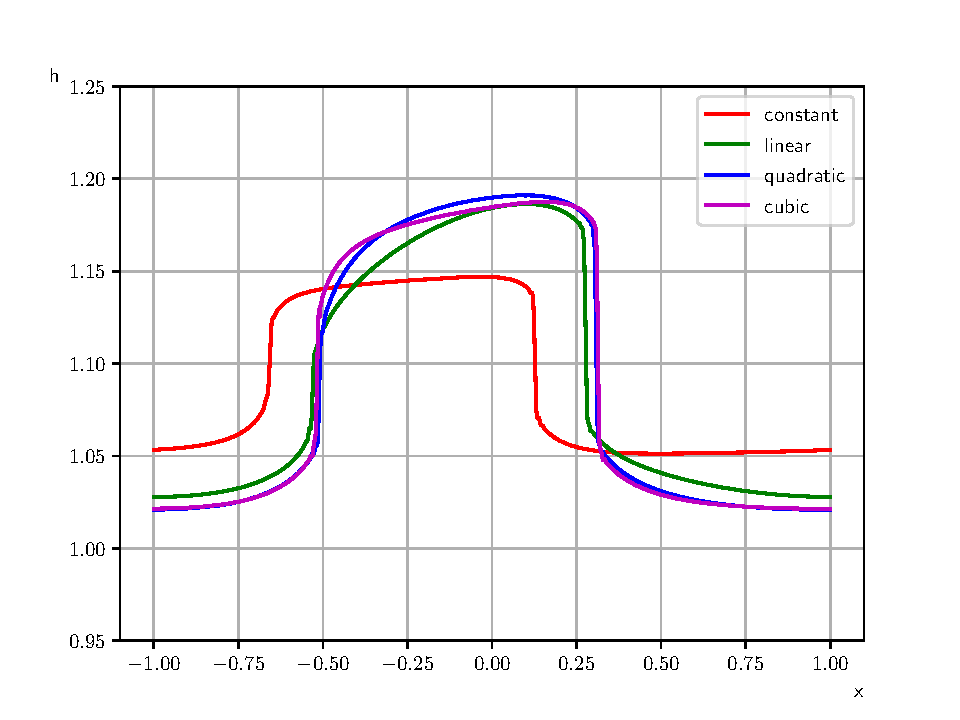
\includegraphics[scale=0.29]{Figures/height_torillhon.pdf}
% 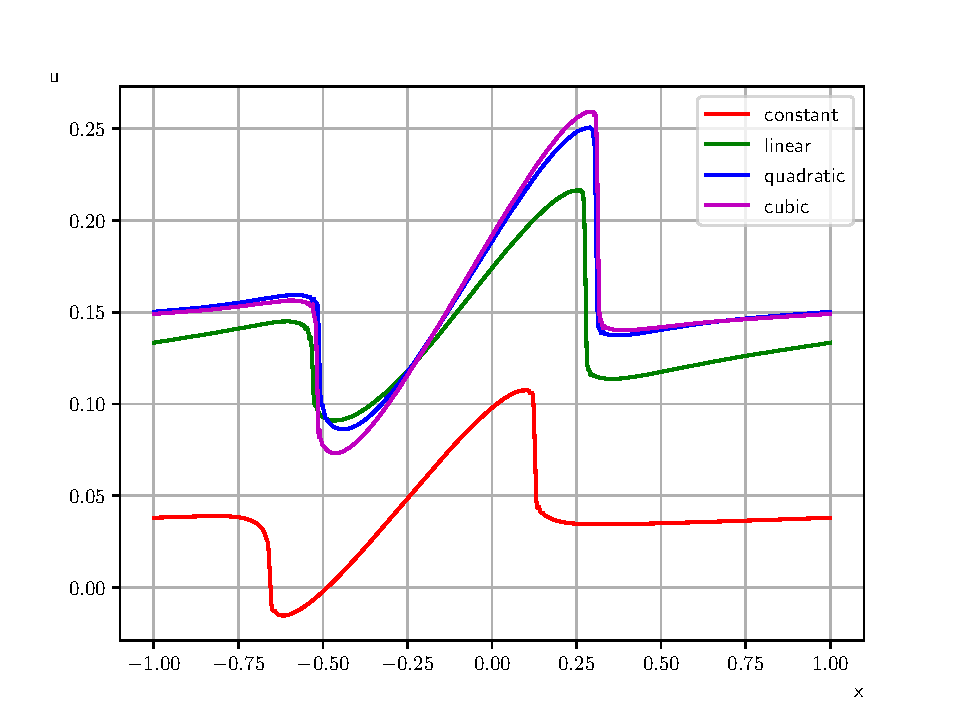
\includegraphics[scale=0.29]{Figures/mean_velocity_torrilhon.pdf}
% 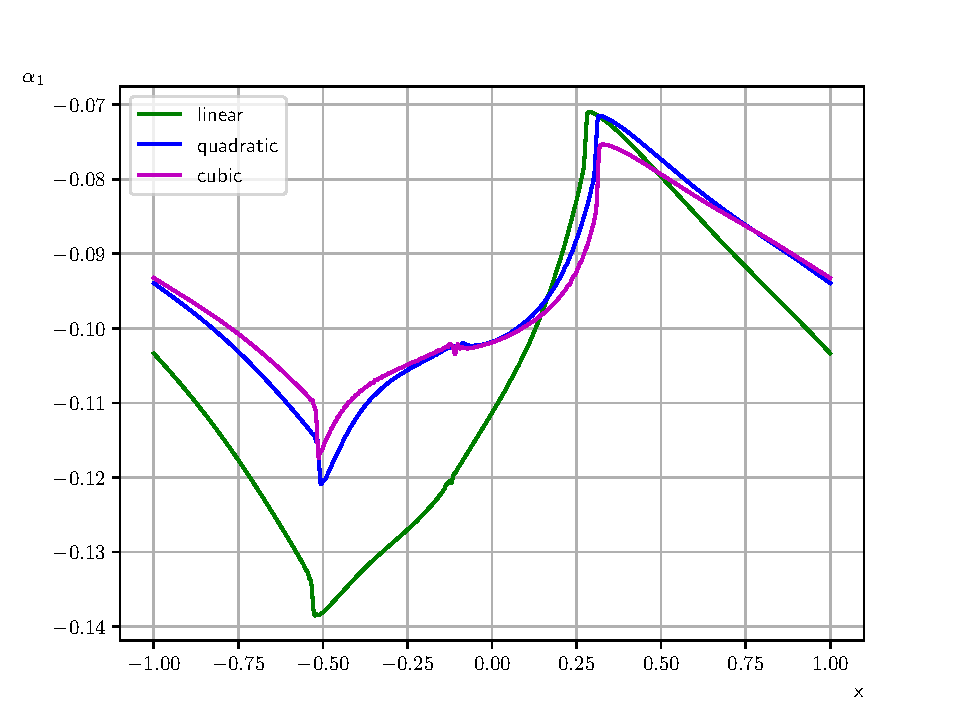
\includegraphics[scale=0.29]{Figures/alpha_1_torrilhon.pdf}
% 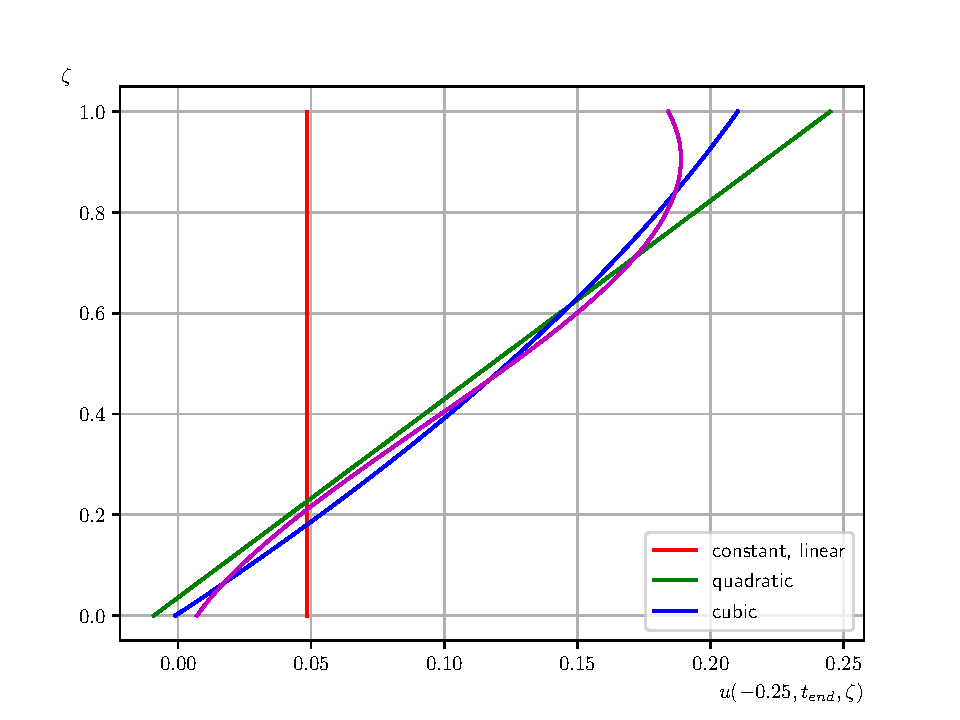
\includegraphics[scale=0.29]{Figures/velocity_profile_-025_torrilhon.pdf}
% 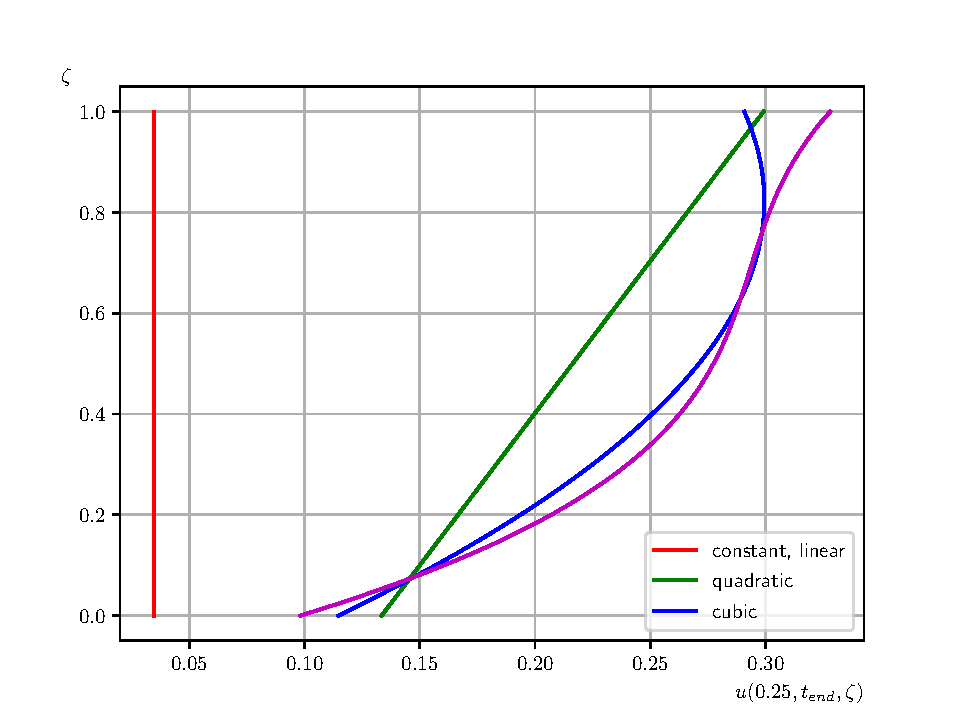
\includegraphics[scale=0.3]{Figures/velocity_profile_025_torrilhon.pdf}

% 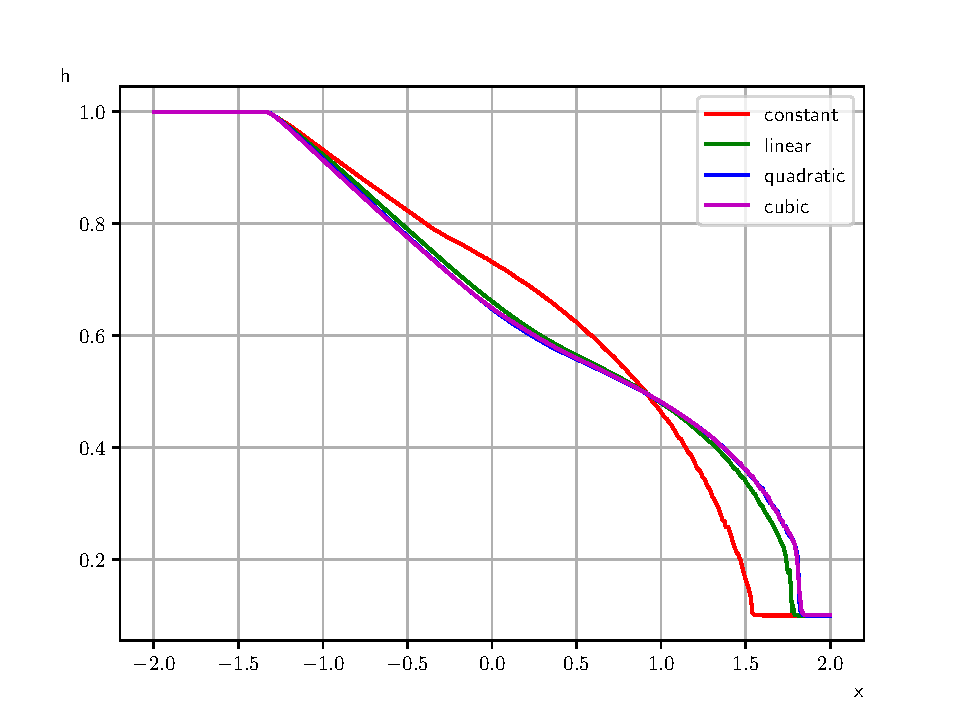
\includegraphics[scale=0.29]{Figures/height_dam.pdf}
% 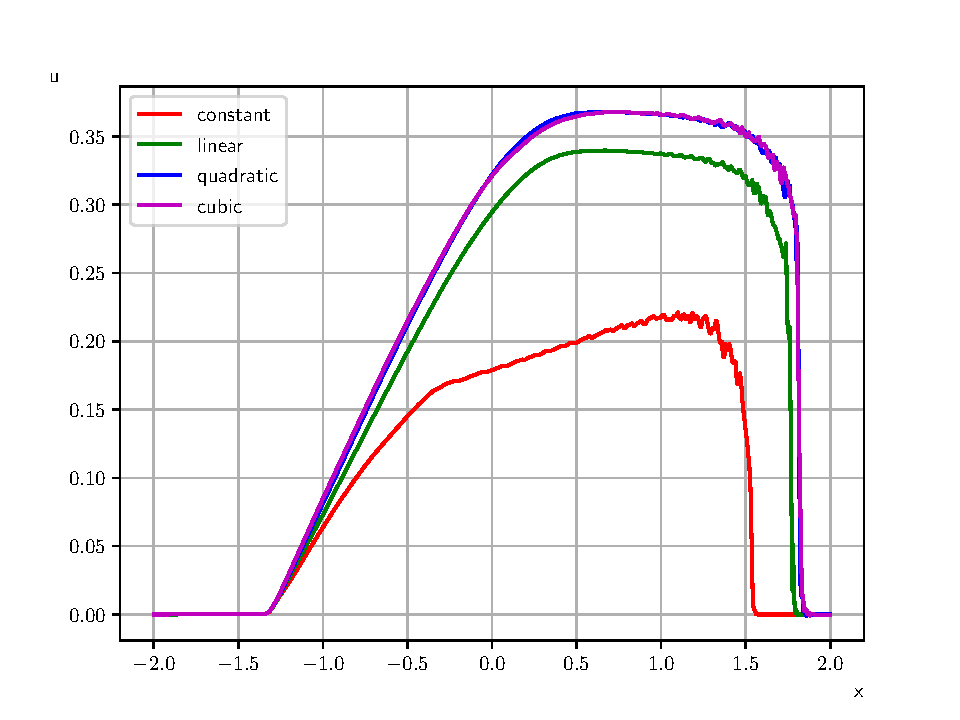
\includegraphics[scale=0.29]{Figures/mean_velocity_dam.pdf}
% 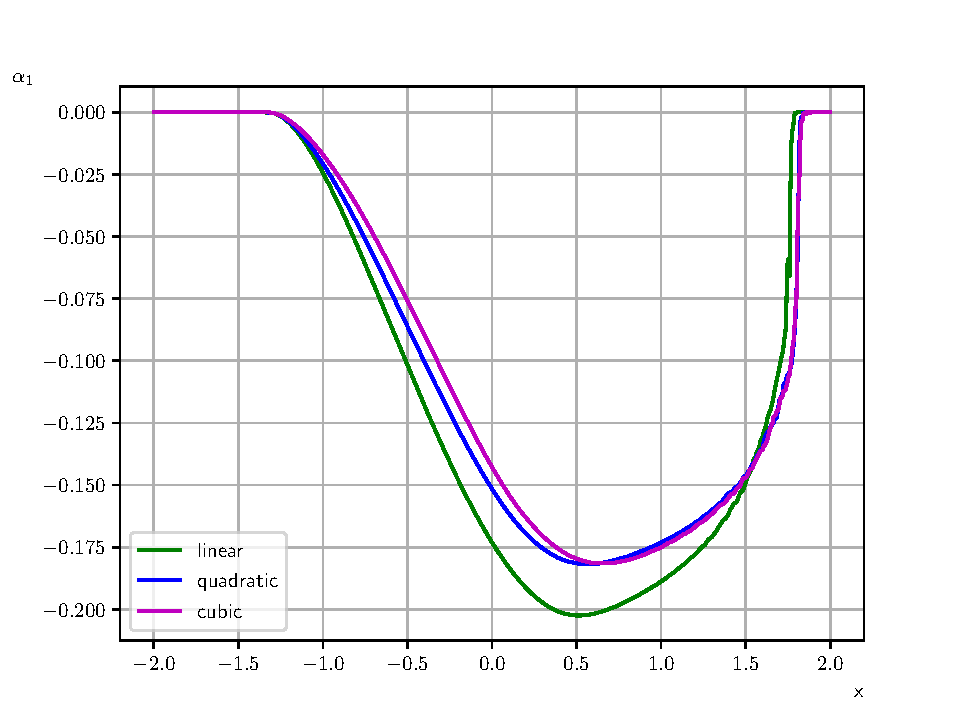
\includegraphics[scale=0.29]{Figures/alpha_1_dam.pdf}
% 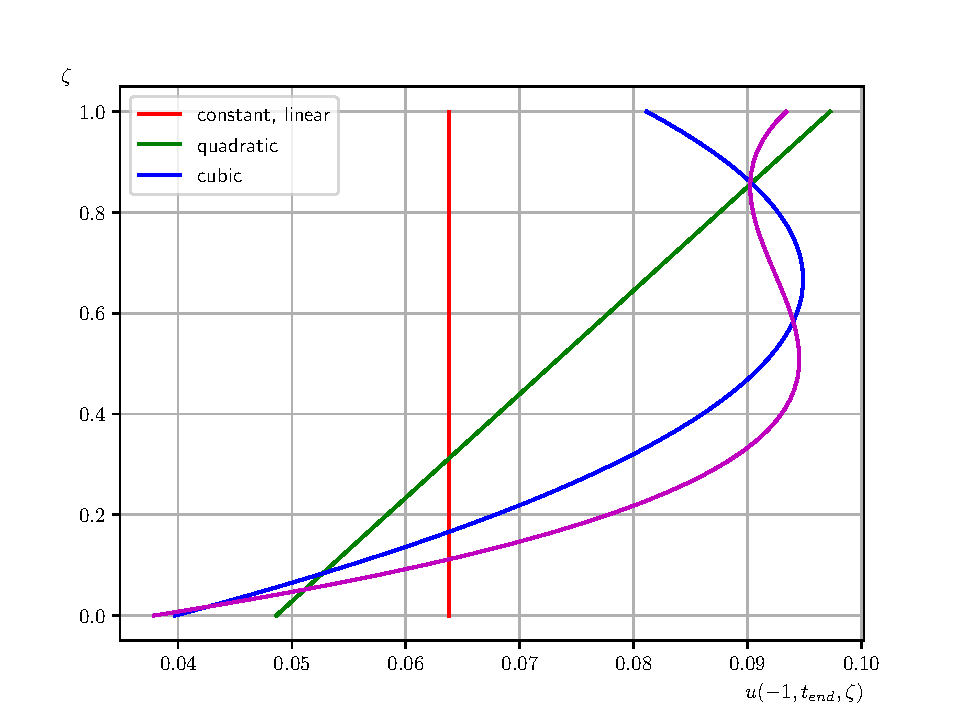
\includegraphics[scale=0.29]{Figures/velocity_profile_-1_dam.pdf}
\subsection{Manufactured Solution}
  I also ran a manufactured solution example to verify the order of convergence of the
  method.
  \begin{gather}
    q_i(x, t) = 0.1 \sin{2 \pi \p{x - t - 0.1 i}}
  \end{gather}
  
  \begin{table}
    \small
    \begin{tabular}{r*{10}l}
      \toprule
            & \multicolumn{2}{c}{1st Order} & \multicolumn{2}{c}{2nd Order} & \multicolumn{2}{c}{3rd Order} & \multicolumn{2}{c}{4th Order} & \multicolumn{2}{c}{5th Order} \\
      \midrule
      \(n\) & \multicolumn{1}{c}{error} & order & \multicolumn{1}{c}{error} & order & \multicolumn{1}{c}{error} & order& \multicolumn{1}{c}{error} & order & \multicolumn{1}{c}{error} & order \\
      \midrule
      20    & \( 0.226 \) & ---  & \( 8.57 \times 10^{-3} \) & ---   & \( 1.67 \times 10^{-4} \) & ---  & \( 3.17 \times 10^{-6}  \) & ---  & \( 7.61 \times 10^{-8}  \) & 0.00  \\
      40    & \( 0.117 \) & 0.96 & \( 2.17 \times 10^{-3} \) & 1.98  & \( 2.07 \times 10^{-5} \) & 3.02 & \( 1.98 \times 10^{-7}  \) & 4.00 & \( 2.38 \times 10^{-9}  \) & 5.00  \\
      80    & \( 0.058 \) & 1.00 & \( 5.40 \times 10^{-4} \) & 2.01  & \( 2.57 \times 10^{-6} \) & 3.01 & \( 1.24 \times 10^{-8}  \) & 4.00 & \( 7.71 \times 10^{-11} \) & 4.95  \\
      160   & \( 0.028 \) & 1.06 & \( 1.35 \times 10^{-4} \) & 2.00  & \( 3.21 \times 10^{-7} \) & 3.00 & \( 7.76 \times 10^{-10} \) & 4.00 & \( 4.04 \times 10^{-11} \) & 0.93  \\
      320   & \( 0.014 \) & 0.99 & \( 3.37 \times 10^{-5} \) & 2.00  & \( 4.01 \times 10^{-8} \) & 3.00 & \( 4.85 \times 10^{-11} \) & 4.00 & \( 8.09 \times 10^{-11} \) & -1.00 \\
      \bottomrule
    \end{tabular}
    \caption{Convergence Table for standard shallow water equations or shallow water moment equations with zero moments.}\label{tab:convergence_1d_0m}
  \end{table}
  \begin{table}
    \small
    \begin{tabular}{r*{10}l}
      \toprule
            & \multicolumn{2}{c}{1st Order} & \multicolumn{2}{c}{2nd Order} & \multicolumn{2}{c}{3rd Order} & \multicolumn{2}{c}{4th Order} & \multicolumn{2}{c}{5th Order} \\
      \midrule
      \(n\) & \multicolumn{1}{c}{error} & order & \multicolumn{1}{c}{error} & order & \multicolumn{1}{c}{error} & order & \multicolumn{1}{c}{error} & order & \multicolumn{1}{c}{error} & order\\
      \midrule
      20    & \( 2.53 \times 10^{-1} \) & ---  & \( 9.97 \times 10^{-3} \) & ---  & \( 1.71 \times 10^{-3} \) & ---  & \( 1.14 \times 10^{-4} \) & ---  & \( 2.68 \times 10^{ -5} \) & ---  \\
      40    & \( 1.30 \times 10^{-1} \) & 0.96 & \( 2.52 \times 10^{-3} \) & 1.98 & \( 3.85 \times 10^{-4} \) & 2.15 & \( 1.74 \times 10^{-5} \) & 2.72 & \( 8.01 \times 10^{ -7} \) & 5.06 \\
      80    & \( 6.47 \times 10^{-2} \) & 1.00 & \( 6.28 \times 10^{-4} \) & 2.00 & \( 6.13 \times 10^{-5} \) & 2.65 & \( 7.50 \times 10^{-7} \) & 4.53 & \( 1.53 \times 10^{ -8} \) & 5.71 \\
      160   & \( 3.13 \times 10^{-2} \) & 1.05 & \( 1.57 \times 10^{-4} \) & 2.00 & \( 9.09 \times 10^{-6} \) & 2.75 & \( 1.25 \times 10^{-7} \) & 2.59 & \( 4.04 \times 10^{-10} \) & 5.25 \\
      320   & \( 1.58 \times 10^{-2} \) & 0.99 & \( 3.92 \times 10^{-5} \) & 2.00 & \( 1.73 \times 10^{-6} \) & 2.39 & \( 8.79 \times 10^{-9} \) & 3.83 & \( 8.40 \times 10^{-11} \) & 2.27 \\
      \bottomrule
    \end{tabular}
    \caption{Convergence table for shallow water moment equations with one moment.}\label{tab:convergence_1d_1m}
  \end{table}
  \begin{table}
    \small
    \centering
    \begin{tabular}{r*{10}l}
      \toprule
            & \multicolumn{2}{c}{1st Order} & \multicolumn{2}{c}{2nd Order} & \multicolumn{2}{c}{3rd Order} & \multicolumn{2}{c}{4th Order} & \multicolumn{2}{c}{5th Order}\\
      \midrule
      \(n\) & \multicolumn{1}{c}{error} & order & \multicolumn{1}{c}{error} & order & \multicolumn{1}{c}{error} & order & \multicolumn{1}{c}{error} & order & \multicolumn{1}{c}{error} & order\\
      \midrule
      20    & \( 2.78 \times 10^{-1} \) & ---  & \( 1.14 \times 10^{-2} \) & ---  & \( 5.35 \times 10^{-3} \) & ---  & \( 3.69 \times 10^{ -4} \) & ---  & \( 5.19 \times 10^{ -5} \) & ---  \\
      40    & \( 1.42 \times 10^{-1} \) & 0.96 & \( 2.88 \times 10^{-3} \) & 1.98 & \( 6.47 \times 10^{-4} \) & 3.05 & \( 2.46 \times 10^{ -5} \) & 3.91 & \( 1.12 \times 10^{ -6} \) & 5.53 \\
      80    & \( 7.12 \times 10^{-2} \) & 1.00 & \( 7.19 \times 10^{-4} \) & 2.00 & \( 7.83 \times 10^{-5} \) & 3.04 & \( 1.40 \times 10^{ -6} \) & 4.13 & \( 1.93 \times 10^{ -8} \) & 5.86 \\
      160   & \( 3.45 \times 10^{-2} \) & 1.04 & \( 1.80 \times 10^{-4} \) & 2.00 & \( 1.27 \times 10^{-5} \) & 2.63 & \( 1.14 \times 10^{ -7} \) & 3.62 & \( 5.86 \times 10^{-10} \) & 5.04 \\
      320   & \( 1.74 \times 10^{-2} \) & 0.99 & \( 4.49 \times 10^{-5} \) & 2.00 & \( 2.55 \times 10^{-6} \) & 2.32 & \( 1.09 \times 10^{ -8} \) & 3.39 & \( 8.79 \times 10^{-11} \) & 2.74 \\
      \bottomrule
    \end{tabular}
    \caption{Convergence table for shallow water moments equations with two moments}\label{tab:convergence_1d_2m}
  \end{table}
  \begin{table}
    \small
    \centering
    \begin{tabular}{r*{10}l}
      \toprule
            & \multicolumn{2}{c}{1st Order} & \multicolumn{2}{c}{2nd Order} & \multicolumn{2}{c}{3rd Order} & \multicolumn{2}{c}{4th Order} & \multicolumn{2}{c}{5th Order} \\
      \midrule
      \(n\) & \multicolumn{1}{c}{error} & order & \multicolumn{1}{c}{error} & order & \multicolumn{1}{c}{error} & order & \multicolumn{1}{c}{error} & order & \multicolumn{1}{c}{error} & order \\
      \midrule
      20    & \( 3.02 \times 10^{-1} \) & ---  & \( 1.30 \times 10^{-2} \) & ---  & \( 7.02 \times 10^{-3} \) & ---  & \( 3.17 \times 10^{ -4} \) & ---  & \( 5.57 \times 10^{ -5} \) & ---  \\
      40    & \( 1.56 \times 10^{-1} \) & 0.96 & \( 3.28 \times 10^{-3} \) & 1.99 & \( 6.99 \times 10^{-4} \) & 3.33 & \( 2.38 \times 10^{ -5} \) & 3.73 & \( 1.10 \times 10^{ -6} \) & 5.66 \\
      80    & \( 7.81 \times 10^{-2} \) & 0.99 & \( 8.19 \times 10^{-4} \) & 2.00 & \( 1.18 \times 10^{-4} \) & 2.56 & \( 2.51 \times 10^{ -6} \) & 3.25 & \( 2.64 \times 10^{ -8} \) & 5.38 \\
      160   & \( 3.80 \times 10^{-2} \) & 1.04 & \( 2.05 \times 10^{-4} \) & 2.00 & \( 2.55 \times 10^{-5} \) & 2.22 & \( 3.17 \times 10^{ -7} \) & 2.99 & \( 1.37 \times 10^{ -9} \) & 4.27 \\
      320   & \( 1.92 \times 10^{-2} \) & 0.99 & \( 5.12 \times 10^{-5} \) & 2.00 & \( 5.11 \times 10^{-6} \) & 2.32 & \( 4.68 \times 10^{ -8} \) & 2.76 & \( 1.17 \times 10^{-10} \) & 3.55 \\
      \bottomrule
    \end{tabular}
    \caption{Convergence table for shallow water moment equations with three moments or a cubic velocity profile}\label{tab:convergence_1d_3m}
  \end{table}

\section{Two Dimensional Cartesian Results}
  \begin{table}
    \small
    \centering
    \begin{tabular}{r*{10}l}
      \toprule
            & \multicolumn{2}{c}{1st Order} & \multicolumn{2}{c}{2nd Order} & \multicolumn{2}{c}{3rd Order} & \multicolumn{2}{c}{4th Order} & \multicolumn{2}{c}{5th Order} \\
      \midrule
      \(n\) & \multicolumn{1}{c}{error} & order & \multicolumn{1}{c}{error} & order & \multicolumn{1}{c}{error} & order & \multicolumn{1}{c}{error} & order & \multicolumn{1}{c}{error} & order \\
      \midrule
      5     & \( 9.26 \times 10^{-1} \) & ---  & \( 9.42 \times 10^{-2} \) & ---  & \( 1.24 \times 10^{-2} \) & ---  & \( 2.25 \times 10^{-3} \) & ---  & \( 4.62 \times 10^{-4} \) & ---  \\
      10    & \( 5.02 \times 10^{-1} \) & 0.88 & \( 2.12 \times 10^{-2} \) & 2.16 & \( 2.77 \times 10^{-3} \) & 2.17 & \( 2.79 \times 10^{-4} \) & 3.02 & \( 4.12 \times 10^{-5} \) & 3.49 \\
      20    & \( 2.79 \times 10^{-1} \) & 0.85 & \( 5.09 \times 10^{-3} \) & 2.06 & \( 7.16 \times 10^{-4} \) & 1.95 & \( 3.43 \times 10^{-5} \) & 3.02 & \( 2.40 \times 10^{-6} \) & 4.10 \\
      40    & \( 1.43 \times 10^{-1} \) & 0.96 & \( 1.26 \times 10^{-3} \) & 2.02 & \( 1.60 \times 10^{-4} \) & 2.16 & \( 3.08 \times 10^{-6} \) & 3.48 & \( 1.23 \times 10^{-7} \) & 4.28 \\
      80    & \( 7.36 \times 10^{-2} \) & 0.96 & \( 3.13 \times 10^{-4} \) & 2.00 & \( 3.37 \times 10^{-5} \) & 2.25 & \( 2.76 \times 10^{-7} \) & 3.48 & \( 6.09 \times 10^{-9} \) & 4.34 \\
      \bottomrule
    \end{tabular}
    \caption{Convergence table for standard shallow water equations or shallow water moment equations with zero moments}\label{tab:convergence_2dr_0m}
  \end{table}

  \begin{table}
    \small
    \centering
    \begin{tabular}{r*{10}l}
      \toprule
            & \multicolumn{2}{c}{1st Order} & \multicolumn{2}{c}{2nd Order} & \multicolumn{2}{c}{3rd Order} & \multicolumn{2}{c}{4th Order} & \multicolumn{2}{c}{5th Order} \\
      \midrule
      \(n\) & \multicolumn{1}{c}{error} & order & \multicolumn{1}{c}{error} & order & \multicolumn{1}{c}{error} & order & \multicolumn{1}{c}{error} & order & \multicolumn{1}{c}{error} & order \\
      \midrule
      5     & \( 1.20 \)                 & ---  & \( 1.16 \times 10^{-1 } \) & ---  & \( 2.07 \times 10^{-2 } \) & ---  & \( 8.11 \times 10^{-3} \) & ---  & \( 1.52 \times 10^{-3} \) & ---  \\
      10    & \( 6.69 \times 10^{-1 } \) & 0.84 & \( 2.46 \times 10^{-2 } \) & 2.24 & \( 7.20 \times 10^{-3 } \) & 1.53 & \( 8.54 \times 10^{-4} \) & 3.25 & \( 1.44 \times 10^{-4} \) & 3.40 \\
      20    & \( 3.81 \times 10^{-1 } \) & 0.81 & \( 5.86 \times 10^{-3 } \) & 2.07 & \( 2.10 \times 10^{-3 } \) & 1.78 & \( 1.14 \times 10^{-4} \) & 2.90 & \( 9.01 \times 10^{-6} \) & 4.00 \\
      40    & \( 2.00 \times 10^{-1 } \) & 0.93 & \( 1.45 \times 10^{-3 } \) & 2.02 & \( 4.78 \times 10^{-4 } \) & 2.13 & \( 1.18 \times 10^{-5} \) & 3.28 & \( 4.62 \times 10^{-7} \) & 4.28 \\
      80    & \( 1.03 \times 10^{-1 } \) & 0.95 & \( 3.61 \times 10^{-4 } \) & 2.00 & \( 1.01 \times 10^{-4 } \) & 2.25 & \( 1.07 \times 10^{-6} \) & 3.47 & \( 2.14 \times 10^{-8} \) & 4.43 \\
      \bottomrule
    \end{tabular}
    \caption{Convergence table for shallow water moment equations with one moment.}\label{tab:convergence_2dr_1m}
  \end{table}

  \begin{table}
    \small
    \centering
    \begin{tabular}{r*{10}l}
      \toprule
            & \multicolumn{2}{c}{1st Order} & \multicolumn{2}{c}{2nd Order} & \multicolumn{2}{c}{3rd Order} & \multicolumn{2}{c}{4th Order} & \multicolumn{2}{c}{5th Order} \\
      \midrule
      \(n\) & \multicolumn{1}{c}{error} & order & \multicolumn{1}{c}{error} & order & \multicolumn{1}{c}{error} & order & \multicolumn{1}{c}{error} & order & \multicolumn{1}{c}{error} & order \\
      \midrule
      5     & \( 1.42 \)                & ---  & \( 1.40 \times 10^{-1} \) & ---  & \( 2.77 \times 10^{-2} \) & ---  & \( 1.08 \times 10^{-2} \) & ---  & \( 2.24 \times 10^{-3} \) & ---  \\
      10    & \( 8.01 \times 10^{-1} \) & 0.83 & \( 2.95 \times 10^{-2} \) & 2.24 & \( 1.04 \times 10^{-2} \) & 1.41 & \( 1.22 \times 10^{-3} \) & 3.15 & \( 2.08 \times 10^{-4} \) & 3.43 \\
      20    & \( 4.62 \times 10^{-1} \) & 0.80 & \( 7.01 \times 10^{-3} \) & 2.07 & \( 2.98 \times 10^{-3} \) & 1.81 & \( 1.62 \times 10^{-4} \) & 2.91 & \( 1.22 \times 10^{-5} \) & 4.09 \\
      40    & \( 2.44 \times 10^{-1} \) & 0.92 & \( 1.73 \times 10^{-3} \) & 2.02 & \( 6.60 \times 10^{-4} \) & 2.18 & \( 1.57 \times 10^{-5} \) & 3.37 & \( 6.11 \times 10^{-7} \) & 4.32 \\
      80    & \( 1.26 \times 10^{-1} \) & 0.95 & \( 4.33 \times 10^{-4} \) & 2.00 & \( 1.37 \times 10^{-4} \) & 2.27 & \( 1.42 \times 10^{-6} \) & 3.47 & \( 2.86 \times 10^{-8} \) & 4.42 \\
      \bottomrule
    \end{tabular}
    \caption{Convergence table for shallow water moment equations with two moments}\label{tab:convergence_2dr_2m}
  \end{table}

\section{Two Dimensional Unstructured Results}
%\chapterbib

%\bibliographystyle{apa}
%\bibliography{Reference/mybib}

% OLD TABLES
  % \begin{table}
  %   \small
  %   \centering
  %   \begin{tabular}{r*{10}l}
  %     \toprule
  %           & \multicolumn{2}{c}{1st Order} & \multicolumn{2}{c}{2nd Order} & \multicolumn{2}{c}{3rd Order} & \multicolumn{2}{c}{4th Order} & \multicolumn{2}{c}{5th Order} \\
  %     \midrule
  %     \(n\) & \multicolumn{1}{c}{error} & order & \multicolumn{1}{c}{error} & order & \multicolumn{1}{c}{error} & order & \multicolumn{1}{c}{error} & order & \multicolumn{1}{c}{error} & order \\
  %     \midrule
  %     20    & \( 3.024 \times 10^{-1} \) & ---  & \( 1.300 \times 10^{-2} \) & ---  & \( 7.015 \times 10^{-3} \) & ---  & \( 3.167 \times 10^{ -4} \) & ---  & \( 5.571 \times 10^{ -5} \) & ---  \\
  %     40    & \( 1.556 \times 10^{-1} \) & 0.96 & \( 3.283 \times 10^{-3} \) & 1.99 & \( 6.992 \times 10^{-4} \) & 3.33 & \( 2.384 \times 10^{ -5} \) & 3.73 & \( 1.099 \times 10^{ -6} \) & 5.66 \\
  %     80    & \( 7.808 \times 10^{-2} \) & 0.99 & \( 8.188 \times 10^{-4} \) & 2.00 & \( 1.183 \times 10^{-4} \) & 2.56 & \( 2.509 \times 10^{ -6} \) & 3.25 & \( 2.639 \times 10^{ -8} \) & 5.38 \\
  %     160   & \( 3.802 \times 10^{-2} \) & 1.04 & \( 2.046 \times 10^{-4} \) & 2.00 & \( 2.545 \times 10^{-5} \) & 2.22 & \( 3.168 \times 10^{ -7} \) & 2.99 & \( 1.371 \times 10^{ -9} \) & 4.27 \\
  %     320   & \( 1.916 \times 10^{-2} \) & 0.99 & \( 5.117 \times 10^{-5} \) & 2.00 & \( 5.110 \times 10^{-6} \) & 2.32 & \( 4.675 \times 10^{ -8} \) & 2.76 & \( 1.171 \times 10^{-10} \) & 3.55 \\
  %     \bottomrule
  %   \end{tabular}
  %   \caption{Convergence table for shallow water moment equations with three moments or a cubic velocity profile}\label{tab:convergence_1d_3m}
  % \end{table}

  % \begin{table}
  %   \centering
  %   \begin{tabular}{r*{10}l}
  %     \toprule
  %           & \multicolumn{2}{c}{1st Order} & \multicolumn{2}{c}{2nd Order} & \multicolumn{2}{c}{3rd Order} & \multicolumn{2}{c}{4th Order} & \multicolumn{2}{c}{5th Order}\\
  %     \midrule
  %     \(n\) & \multicolumn{1}{c}{error} & order & \multicolumn{1}{c}{error} & order & \multicolumn{1}{c}{error} & order & \multicolumn{1}{c}{error} & order & \multicolumn{1}{c}{error} & order\\
  %     \midrule
  %     20    & \( 2.778 \times 10^{-1} \) & ---  & \( 1.141 \times 10^{-2} \) & ---  & \( 5.350 \times 10^{-3} \) & ---  & \( 3.688 \times 10^{ -4} \) & ---  & \( 5.194 \times 10^{ -5} \) & ---  \\
  %     40    & \( 1.424 \times 10^{-1} \) & 0.96 & \( 2.884 \times 10^{-3} \) & 1.98 & \( 6.466 \times 10^{-4} \) & 3.05 & \( 2.461 \times 10^{ -5} \) & 3.91 & \( 1.121 \times 10^{ -6} \) & 5.53 \\
  %     80    & \( 7.121 \times 10^{-2} \) & 1.00 & \( 7.191 \times 10^{-4} \) & 2.00 & \( 7.836 \times 10^{-5} \) & 3.04 & \( 1.403 \times 10^{ -6} \) & 4.13 & \( 1.934 \times 10^{ -8} \) & 5.86 \\
  %     160   & \( 3.454 \times 10^{-2} \) & 1.04 & \( 1.797 \times 10^{-4} \) & 2.00 & \( 1.270 \times 10^{-5} \) & 2.63 & \( 1.144 \times 10^{ -7} \) & 3.62 & \( 5.859 \times 10^{-10} \) & 5.04 \\
  %     320   & \( 1.740 \times 10^{-2} \) & 0.99 & \( 4.493 \times 10^{-5} \) & 2.00 & \( 2.546 \times 10^{-6} \) & 2.32 & \( 1.092 \times 10^{ -8} \) & 3.39 & \( 8.791 \times 10^{-11} \) & 2.74 \\
  %     \bottomrule
  %   \end{tabular}
  %   \caption{Convergence table for shallow water moments equations with two moments}\label{tab:convergence_1d_2m}
  % \end{table}
  % \begin{table}
  %   \begin{tabular}{r*{10}l}
  %     \toprule
  %           & \multicolumn{2}{c}{1st Order} & \multicolumn{2}{c}{2nd Order} & \multicolumn{2}{c}{3rd Order} & \multicolumn{2}{c}{4th Order} & \multicolumn{2}{c}{5th Order} \\
  %     \midrule
  %     \(n\) & \multicolumn{1}{c}{error} & order & \multicolumn{1}{c}{error} & order & \multicolumn{1}{c}{error} & order& \multicolumn{1}{c}{error} & order & \multicolumn{1}{c}{error} & order \\
  %     \midrule
  %     20    & \( 0.226 \) & ---  & \( 8.57 \times 10^{-3} \) & ---   & \( 1.67 \times 10^{-4} \) & ---  & \( 3.172 \times 10^{-6}  \) & ---  & \( 7.606 \times 10^{-8}  \) & 0.00  \\
  %     40    & \( 0.117 \) & 0.96 & \( 2.17 \times 10^{-3} \) & 1.98  & \( 2.07 \times 10^{-5} \) & 3.02 & \( 1.982 \times 10^{-7}  \) & 4.00 & \( 2.380 \times 10^{-9}  \) & 5.00  \\
  %     80    & \( 0.058 \) & 1.00 & \( 5.40 \times 10^{-4} \) & 2.01  & \( 2.57 \times 10^{-6} \) & 3.01 & \( 1.240 \times 10^{-8}  \) & 4.00 & \( 7.713 \times 10^{-11} \) & 4.95  \\
  %     160   & \( 0.028 \) & 1.06 & \( 1.35 \times 10^{-4} \) & 2.00  & \( 3.21 \times 10^{-7} \) & 3.00 & \( 7.755 \times 10^{-10} \) & 4.00 & \( 4.035 \times 10^{-11} \) & 0.93  \\
  %     320   & \( 0.014 \) & 0.99 & \( 3.37 \times 10^{-5} \) & 2.00  & \( 4.01 \times 10^{-8} \) & 3.00 & \( 4.849 \times 10^{-11} \) & 4.00 & \( 8.085 \times 10^{-11} \) & -1.00 \\
  %     \bottomrule
  %   \end{tabular}
  %   \caption{Convergence Table for standard shallow water equations or shallow water moment equations with zero moments.}\label{tab:convergence_1d_0m}
  % \end{table}
  % \begin{table}
  %   \centering
  %   \begin{tabular}{r*{10}l}
  %     \toprule
  %           & \multicolumn{2}{c}{1st Order} & \multicolumn{2}{c}{2nd Order} & \multicolumn{2}{c}{3rd Order} & \multicolumn{2}{c}{4th Order} & \multicolumn{2}{c}{5th Order} \\
  %     \midrule
  %     \(n\) & \multicolumn{1}{c}{error} & order & \multicolumn{1}{c}{error} & order & \multicolumn{1}{c}{error} & order & \multicolumn{1}{c}{error} & order & \multicolumn{1}{c}{error} & order \\
  %     \midrule
  %     5     & \( 9.259 \times 10^{-1} \) & ---  & \( 9.423 \times 10^{-2} \) & ---  & \( 1.243 \times 10^{-2} \) & ---  & \( 2.254\times 10^{-3} \) & ---  & \( 4.623\times 10^{-4} \) & ---  \\
  %     10    & \( 5.016 \times 10^{-1} \) & 0.88 & \( 2.115 \times 10^{-2} \) & 2.16 & \( 2.769 \times 10^{-3} \) & 2.17 & \( 2.787\times 10^{-4} \) & 3.02 & \( 4.121\times 10^{-5} \) & 3.49 \\
  %     20    & \( 2.786 \times 10^{-1} \) & 0.85 & \( 5.089 \times 10^{-3} \) & 2.06 & \( 7.163 \times 10^{-4} \) & 1.95 & \( 3.434\times 10^{-5} \) & 3.02 & \( 2.395\times 10^{-6} \) & 4.10 \\
  %     40    & \( 1.434 \times 10^{-1} \) & 0.96 & \( 1.257 \times 10^{-3} \) & 2.02 & \( 1.600 \times 10^{-4} \) & 2.16 & \( 3.075\times 10^{-6} \) & 3.48 & \( 1.234\times 10^{-7} \) & 4.28 \\
  %     80    & \( 7.355 \times 10^{-2} \) & 0.96 & \( 3.133 \times 10^{-4} \) & 2.00 & \( 3.367 \times 10^{-5} \) & 2.25 & \( 2.762\times 10^{-7} \) & 3.48 & \( 6.087\times 10^{-9} \) & 4.34 \\
  %     \bottomrule
  %   \end{tabular}
  %   \caption{Convergence table for standard shallow water equations or shallow water moment equations with zero moments}\label{tab:convergence_2dr_0m}
  % \end{table}

  % \begin{table}
  %   \centering
  %   \begin{tabular}{r*{10}l}
  %     \toprule
  %           & \multicolumn{2}{c}{1st Order} & \multicolumn{2}{c}{2nd Order} & \multicolumn{2}{c}{3rd Order} & \multicolumn{2}{c}{4th Order} & \multicolumn{2}{c}{5th Order} \\
  %     \midrule
  %     \(n\) & \multicolumn{1}{c}{error} & order & \multicolumn{1}{c}{error} & order & \multicolumn{1}{c}{error} & order & \multicolumn{1}{c}{error} & order & \multicolumn{1}{c}{error} & order \\
  %     \midrule
  %     5     & \( 1.199 \)                 & ---  & \( 1.159 \times 10^{-1 } \) & ---  & \( 2.073 \times 10^{-2 } \) & ---  & \( 8.114 \times 10^{-3} \) & ---  & \( 1.520 \times 10^{-3} \) & ---  \\
  %     10    & \( 6.686 \times 10^{-1 } \) & 0.84 & \( 2.459 \times 10^{-2 } \) & 2.24 & \( 7.202 \times 10^{-3 } \) & 1.53 & \( 8.542 \times 10^{-4} \) & 3.25 & \( 1.437 \times 10^{-4} \) & 3.40 \\
  %     20    & \( 3.813 \times 10^{-1 } \) & 0.81 & \( 5.857 \times 10^{-3 } \) & 2.07 & \( 2.096 \times 10^{-3 } \) & 1.78 & \( 1.143 \times 10^{-4} \) & 2.90 & \( 9.013 \times 10^{-6} \) & 4.00 \\
  %     40    & \( 1.995 \times 10^{-1 } \) & 0.93 & \( 1.448 \times 10^{-3 } \) & 2.02 & \( 4.777 \times 10^{-4 } \) & 2.13 & \( 1.180 \times 10^{-5} \) & 3.28 & \( 4.625 \times 10^{-7} \) & 4.28 \\
  %     80    & \( 1.033 \times 10^{-1 } \) & 0.95 & \( 3.614 \times 10^{-4 } \) & 2.00 & \( 1.005 \times 10^{-4 } \) & 2.25 & \( 1.068 \times 10^{-6} \) & 3.47 & \( 2.143 \times 10^{-8} \) & 4.43 \\
  %     \bottomrule
  %   \end{tabular}
  %   \caption{Convergence table for shallow water moment equations with one moment.}\label{tab:convergence_2dr_1m}
  % \end{table}

  % \begin{table}
  %   \centering
  %   \begin{tabular}{r*{10}l}
  %     \toprule
  %           & \multicolumn{2}{c}{1st Order} & \multicolumn{2}{c}{2nd Order} & \multicolumn{2}{c}{3rd Order} & \multicolumn{2}{c}{4th Order} & \multicolumn{2}{c}{5th Order} \\
  %     \midrule
  %     \(n\) & \multicolumn{1}{c}{error} & order & \multicolumn{1}{c}{error} & order & \multicolumn{1}{c}{error} & order & \multicolumn{1}{c}{error} & order & \multicolumn{1}{c}{error} & order \\
  %     \midrule
  %     5     & \( 1.420 \)                & ---  & \( 1.399 \times 10^{-1} \) & ---  & \( 2.770 \times 10^{-2} \) & ---  & \( 1.076 \times 10^{-2} \) & ---  & \( 2.236 \times 10^{-3} \) & ---  \\
  %     10    & \( 8.013 \times 10^{-1} \) & 0.83 & \( 2.951 \times 10^{-2} \) & 2.24 & \( 1.043 \times 10^{-2} \) & 1.41 & \( 1.216 \times 10^{-3} \) & 3.15 & \( 2.078 \times 10^{-4} \) & 3.43 \\
  %     20    & \( 4.615 \times 10^{-1} \) & 0.80 & \( 7.011 \times 10^{-3} \) & 2.07 & \( 2.982 \times 10^{-3} \) & 1.81 & \( 1.618 \times 10^{-4} \) & 2.91 & \( 1.224 \times 10^{-5} \) & 4.09 \\
  %     40    & \( 2.436 \times 10^{-1} \) & 0.92 & \( 1.733 \times 10^{-3} \) & 2.02 & \( 6.596 \times 10^{-4} \) & 2.18 & \( 1.566 \times 10^{-5} \) & 3.37 & \( 6.114 \times 10^{-7} \) & 4.32 \\
  %     80    & \( 1.264 \times 10^{-1} \) & 0.95 & \( 4.327 \times 10^{-4} \) & 2.00 & \( 1.365 \times 10^{-4} \) & 2.27 & \( 1.418 \times 10^{-6} \) & 3.47 & \( 2.859 \times 10^{-8} \) & 4.42 \\
  %     \bottomrule
  %   \end{tabular}
  %   \caption{Convergence table for shallow water moment equations with two moments}\label{tab:convergence_2dr_2m}
  % \end{table}
% Chapter 5 from the standard thesis template
%   with a full page figure and a sideways table.
\chapter{Conclusion}

\section{Summary}
  
\section{Future Work}

%\chapterbib

%\bibliographystyle{apa}
%\bibliography{Reference/mybib}

%% Rearranging the table of contents to show references before appendix
%\unappendixtitle
%\addcontentsline{toc}{chapter}{REFERENCES} %this line is to be included before the last chapter so that in toc it appears after the last chapter. If you want the reference to be the last entry of the toc, remove this line and in the biblio.tex file insert this line (or uncomment the line  )

%% An example bibliography from the standard thesis template
\renewcommand{\bibname}{\centerline{REFERENCES}}
\unappendixtitle
\interlinepenalty=300
% For no page break use thebibnopage environment
\begin{thebibliography}{99}
%\begin{singlespacing}
\begingroup
    \setlength{\bibsep}{13.2pt}
  \linespread{1}\selectfont
\addcontentsline{toc}{chapter}{REFERENCESets}

\bibitem[Allen, B.~S.~(1984)]{allen}
Allen, B.~S. (1984). System-assigned learning strategies and CBI.
\emph{Journal of Instructional Computing Research},
\emph{1}(1), 3--18.
\filbreak

\bibitem[Bruner, J.~(1960)]{bruner}
Bruner, J. (1960). \emph{The process of education}.
New York: Random House.
\filbreak

\bibitem[Cox, S.~R.~(1974)]{cox}
Cox, S.~R. (1974). Computer-assisted instruction and student performance
in macroeconomic principles.
\emph{The Journal of Economic Education},
\emph{6}(1), 29--37.
\filbreak
%\end{singlespacing}
\end{thebibliography}

\renewcommand{\bibname}{\centerline{BIBLIOGRAPHY}}
\unappendixtitle
\interlinepenalty=300
\newpage
\phantomsection
\begingroup
    \setlength{\bibsep}{13.2pt}
  \linespread{1}\selectfont
\addcontentsline{toc}{chapter}{BIBLIOGRAPHY}
\bibliography{Reference/mybib}
\unappendixtitle
\endgroup



% % Appendix1 file from standard thesis template

\appendixtitle 
\appendix


%% Use the following two lines for single appendix
%\unappendixtitle
%\singleappendixtitle

\chapter{ADDITIONAL MATERIAL} 
This is now the same as any other chapter except that
all sectioning levels below the chapter level must begin
with the *-form of a sectioning command.

\section*{More stuff}

Supplemental material.


% Instruction for single appendix check instruction in Appendix/appendix1.tex on top of the file
% % An example second appendix from the example thesis thesis.tex.
\chapter{STATISTICAL RESULTS}

This is now the same as any other chapter except that
all sectioning levels below the chapter level must begin
with the *-form of a sectioning command.

\section*{Supplemental Statistics}

More stuff.


\end{document}

% IMPORTANT NOTES
% TABLE OF CONTENTS :
% TOPIC 1:  If you need a page break follow the steps below
% step1
% check before which chapter in the table of contents you want a page break
% step 2
% go the folder "body". There open the chapter tex file that you noted needed page break in the table of contents..
% step 3
% insert  \addtocontents{toc}{\protect\newpage} before the first line i.e. before the line \chapter{RESULTS}.

%%%%%%%%%%%%%%%%%%%%%%%%%%%%
% \def\@makechapterhead#1{%
% IN ORDER TO MAKE spacing changes in the title page got to the section in the isuthesis.cls file
% that starts with \long\def\maketitle{\begin{titlepage} and you can use options like
% singlespace (less spacing)
%singlespacing (comparitively more spacing almost like 2 spacing)
% onehalfspacing
%doublespacing (this is more spacing than the singlespacing above )
% more definitions on spacing can be found by going through the class file


% use \isucaption{} for all captions of figures and tables, where the captions are not too long.

% Use \isucaption[]{} with the square brackets for short caption of figure or table that goes into the list of tables and list of figures, and the curly brackets can have long captions which go with the figure/ table.

%%%%%% Using sub figures
% %%% In preamble include : \usepackage{subfig}
% \begin{figure}[htbp]
% 	\centering
% 	\subfloat[first caption.\label{fig:2a}]{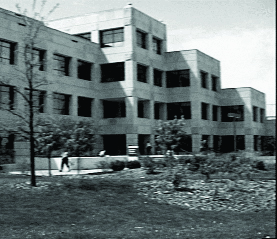
\includegraphics[width=0.2\textwidth]{Images/dc5.jpg}}\hfill
%     \subfloat[second caption.\label{fig:2b}] {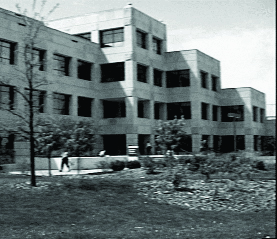
\includegraphics[width=0.2\textwidth]{Images/dc5.jpg}}\hfill
% 	\isucaption{Sub-figure test}
% 	\label{fig:subfigure-test}
% \end{figure}

% Subfloat reference: Fig \ref{fig:2a}

% Figure reference: Fig \ref{fig:subfigure-test}
